\chapter{Results}

%In this section you discuss any issues that came up while developing the system.  If you found something particularly interesting, difficult, or an important learning experience, put it here.  This is also a good place to put additional figures and data.


\textbf{Tala um raunverulega ásæðu af hverju ég vel þessa íhluti!!!!!!}

\section{Hydrophone}

\textbf{TALA UM AÐRA TÝPU SEM HEFÐI GETAÐ KOMIÐ TIL GREINA
https://www.nauta-rcs.it/English/Instruments/Hydrophones/CetaceanResearchTech/C55/C55.html}

First thing that needed to be determined was the hydrophone used.
Generally hydrophones are sensitive piezoelectric sensors that can detect small changes in pressure and convert that to electrical signal.
This project will use the Aquarian audio H1a for its low cost and good sensitivity as well as it was readily available at the Reykjavik University lab.

\begin{table}[h]\caption{Important specifications of the Aquarian H1a hydrophone.\cite{noauthor_aquarian_nodate}}.\label{Tab:Aquarian}
\begin{tabular}{l|l}
Sensitivity     & -190dB re: 1V/µPa (+/- 4dB 20Hz-4KHz) \\\hline
Useful range    & \begin{tabular}[c]{@{}l@{}}100KHz (not measured above 100KHz, approximate sensitivity\\  @100KHz = -220dB re: 1V/µPa)\end{tabular} \\\hline
Capacitance     & 25nF \\ \hline
Operating depth & \textless{}80meters\\ \hline
Cost            &  159\$ \\ \hline
\end{tabular}
\end{table}

There is no preamplifier or impedance buffer circuit within the Aquarian H1a hydrophone, so the circuit needs to amplify the output signal of the hydrophone.
The gain of the circuit depends on what the intended use of the hydrophone will be.
In this case for cetaceans and large aquatic wildlife, Aquarian recommends gain of 40 - 50 dB and for very distant sounds 60dB.

\begin{equation}
F_c = 1 / 0.000000157 * R  
\label{eq:fchydro}
\end{equation}

The Frequency response of the Aquarian H1a hydrophone can be calculated using \textit{Equation~\ref{eq:fchydro}} \cite{noauthor_aquarian_nodate}. 
Which is just \textit{Equation~\ref{eq:FC}} where the capacitance of the hydrophone has been added to it.


\subsection{Microcontroller og ADC}

\textbf{TALA UM TEENSY 3.5 og https://www.pjrc.com/teensy/K64P144M120SF5.pdf
}
\subsubsection{Microcontroller}
The Teensy3.5 was ultimately chosen for the microcontroller of the system.fa
This decision was made for several reasons.
The Teensy3.5 has two built-in ADC, which means the system might be able to add another hydrophone to it for recording.
Both ADCs have a maximum resolution of 16bits with a voltage range of 0 - 3.3V, or $\frac{3.3}{2^16} \approx 0.00005V \approx 50\mu V$ step size.
The Teensy also consumes little power, when running with no peripherals active the processor is powered roughly by 0.5mA or 0.165W.
Which is under the requirements set in the beginning of the project.
As well as it was readily available at the Reykjavik University lab.

\subsubsection{Operational amplifier}
\textbf{Mögulega tala um í kafla 2 hvað mikilvægustu þáttir opampa fyrir þetta verkefni var}

The operational amplifier that was chosen for this project was the OPA1644 from Texas Instruments.
It was chosen its advertised superior sound quality.
Where the noise is $\frac{5.1nV}{\sqrt{Hz}}$ at 1kHz.
Which means 
%https://www.designnews.com/what-nvvhz-noise
\textbf{KYNNA Sér SNR}
$$\sqrt{100*10^3Hz - 10Hz} = 3\sqrt{11110}Hz$$
$$3\sqrt{11110}Hz*5.1*10^{-9}V = 1.6*10^{-6}V$$
$$ 1.6*10^{-6}V * 100 = 1.6*10^{-4}$$
Using a 1V output (0dBV) from the op amp the signal to noise ratio is:
$$SNR = 20log_{10}(\frac{1V}{1.6*10^{-4}V}) \approx 76dB$$

Low distortion of 0.00005\% at 1 kHz and a high slew rate of $\frac{20V}{\mu s}$.
As well as having a supply range that fits within the voltage range of the Teensy analog pins.
\cite{noauthor_opa164x_nodate}

\begin{figure}[h]
    \centering
    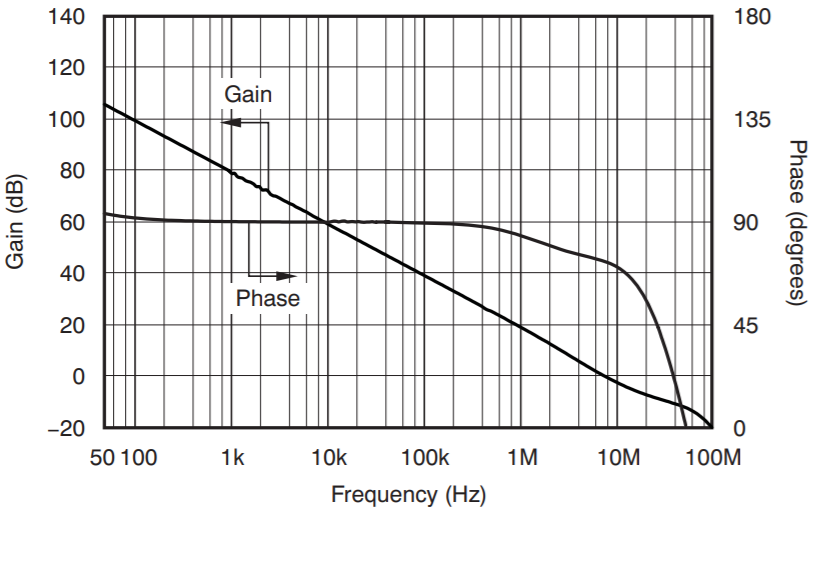
\includegraphics[width=0.7\textwidth]{graphics/dbVsfreq.png}
    \caption{\textbf{BÆTA}}
    \label{fig:dbvsFreq}
\end{figure}

\begin{figure}[h]
    \centering
    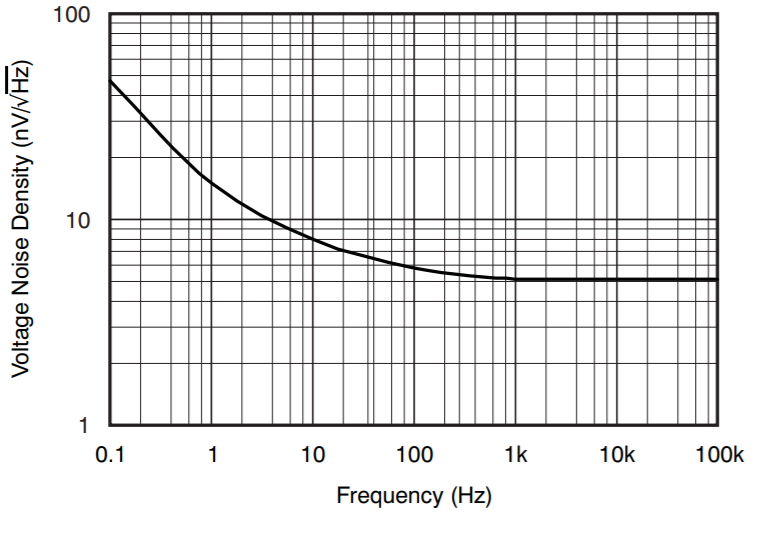
\includegraphics[width=0.7\textwidth]{graphics/noiseDensvsFreq.png}
    \caption{\textbf{BÆTA}}
    \label{fig:noiseDensvsFreq}
\end{figure}

\section{Circuit}

From the project goals the circuit needs to be able to gather data from signals with frequencies between 10 - 100kHz. 
The Aquarian H1a hydrophone data sheet also specifies that for cetacean vocalization recording the gain of the preamplifier needs to be between 40 - 50 dB.
The circuit will there for consist of active low pass filter and high pass filter, a scaling summing amplifier and an inverting op amp.
It will then feed to the Teensy 3.5 built-in ADC.
The setup of the circuit can be seen in \textit{Figures \ref{fig:Opamp1}, \ref{fig:Opamp4}}.
\textit{Figure \ref{fig:Opamp1}} shows the first part of the circuit.
The output of the hydrophone is first connected to a high pass filter, where the capacitance, 25nF of the hydrophone is used as the capacitor in the high pass filter.

\begin{figure}[h]
    \centering
    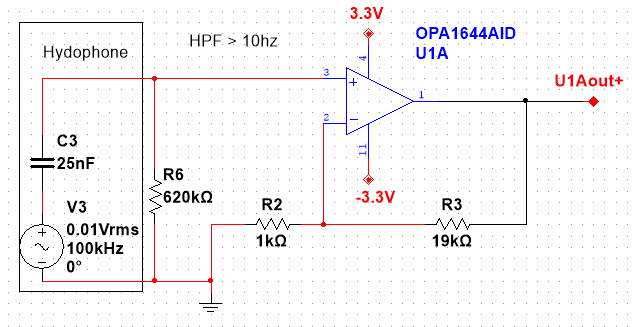
\includegraphics[width=0.70\textwidth]{graphics/OPamp1.png}
    \caption{The first part of the circuit where the output of the hydrophone first filtered using an active high pass filter and then connected to a operational amplifier and amplifying the signal by 20.}
    \label{fig:Opamp1}
\end{figure}


The desired value for the high pass filter was 10Hz and using \textit{Equation~\ref{eq:fchydro}} provided in the data sheet, the resistor value was estimated.   
$$F_c = \frac{1}{0.000000157 * 636k\Omega} = 10Hz$$
Using standard resistor values, the closest resistor value is 620k which yields a cut off frequency of 10.26Hz.
The gain over the active high pass filter can be represented using \textit{Equation \ref{eq:DCGain}} and \textit{Equation \ref{eq:ActiveHighPass}}. 
Where $A_{V1} = 1 + \frac{19k\Omega}{1k\Omega} = 20$.
$$A_f = \frac{(1+\frac{19k}{1k})(\frac{f}{10.26Hz})}{\sqrt{1 + (\frac{f}{10.26Hz})^2}} \approx 20$$
Which is approximately equal to 20, as seen in \textit{Figure~\ref{fig:AVhighpass}} over the entire bandwidth.

\begin{figure}[h]
    \centering
    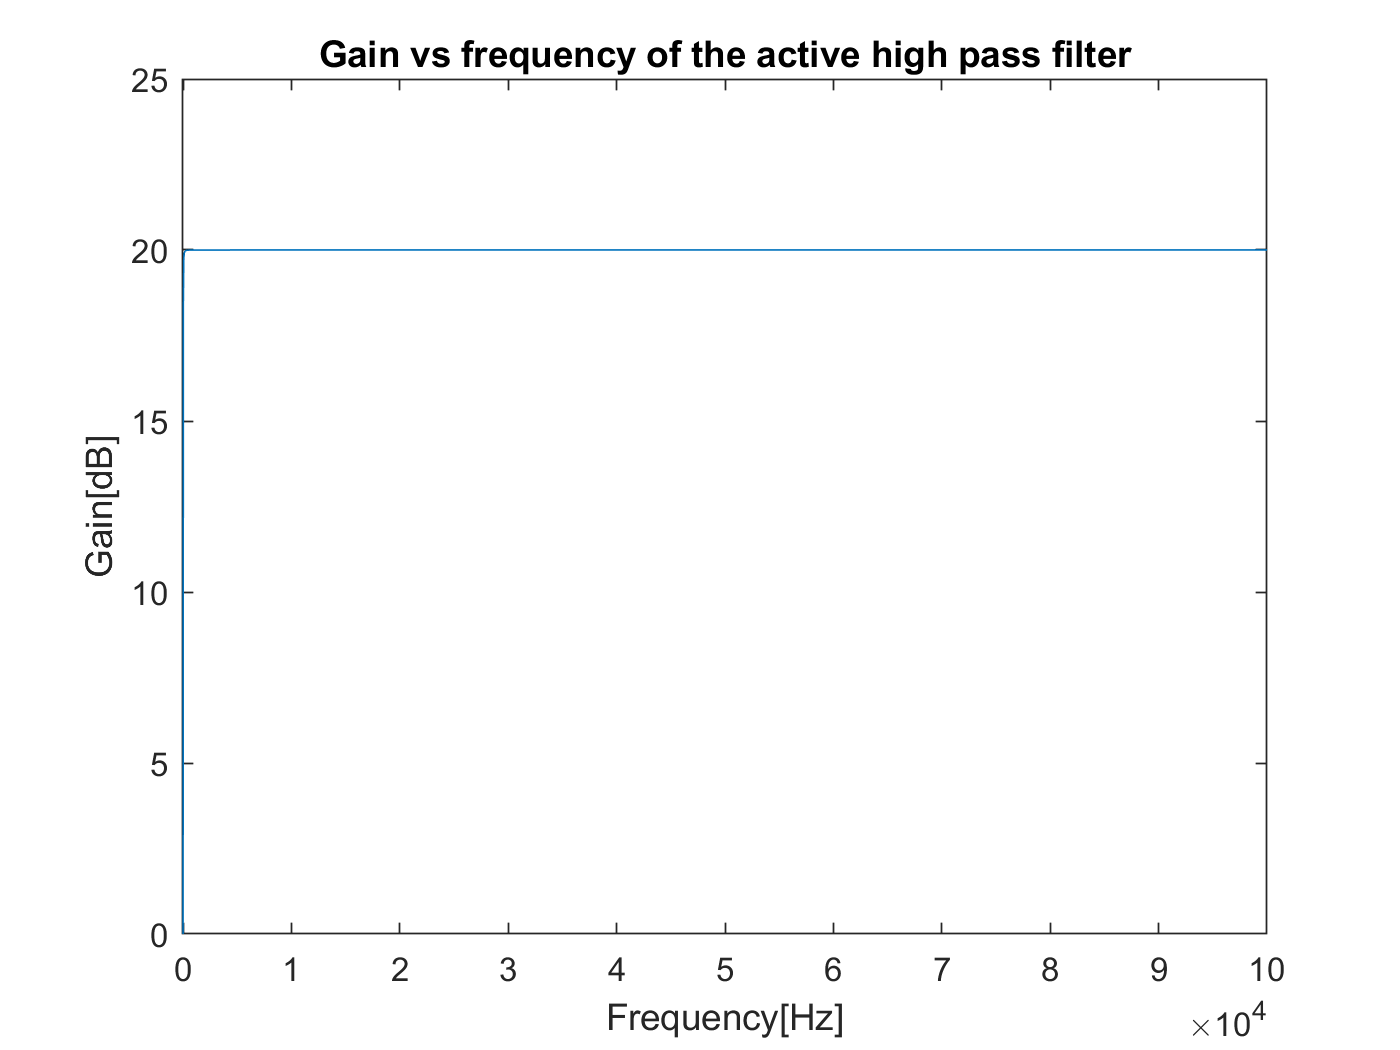
\includegraphics[width=0.7\textwidth]{graphics/Av_Highpass.png}
    \caption{The gain of the operational amplifier with the active high pass filter.}
    \label{fig:AVhighpass}
\end{figure}

\textit{Figure \ref{fig:Opamp2}} shows the active low pass filter configuration which has a cut off frequency of $\approx$ 100kHz and a gain of 2.5.

\begin{figure}[h]
    \centering
    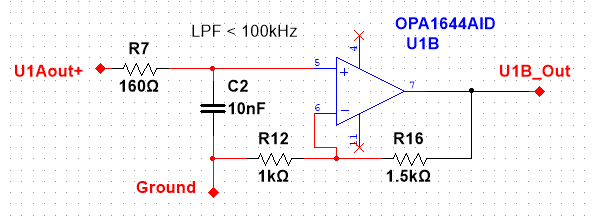
\includegraphics[width=0.7\textwidth]{graphics/OPamp2.png}
    \caption{The second operational amplifier, where the signal is first filtered by the active low pass filter as well as amplifying the signal.}
    \label{fig:Opamp2}
\end{figure}

The desired value for the high pass filter was 100kHz and using \textit{Equation~\ref{eq:FC}} and choosing a resistor value of 160$\Omega$, the capacitor value was estimated.   
$$F_c = \frac{1}{2\pi 9.9nF 160\Omega} = 100kHz$$
Using standard capacitor values, the closest capacitor value is 10nF which yields a cut off frequency of 99472Hz.
The gain over the active low pass filter can be represented using \textit{Equation \ref{eq:DCGain}} and \textit{Equation \ref{eq:ActiveLowPass}}. 
Where $A_{V1} = 1 + \frac{1.5k\Omega}{1k\Omega} = 2.5$.
$$A_f  = \frac{1 + \frac{1.5k\Omega}{1k\Omega}}{\sqrt{1 + (\frac{f}{99471.8Hz})^2}}$$
Which is approximately equal to 2.5 with frequencies until 20kHz, as seen in 
\textit{Figure~\ref{fig:AVlowpass}}.
\\
\begin{figure}[h]
    \centering
    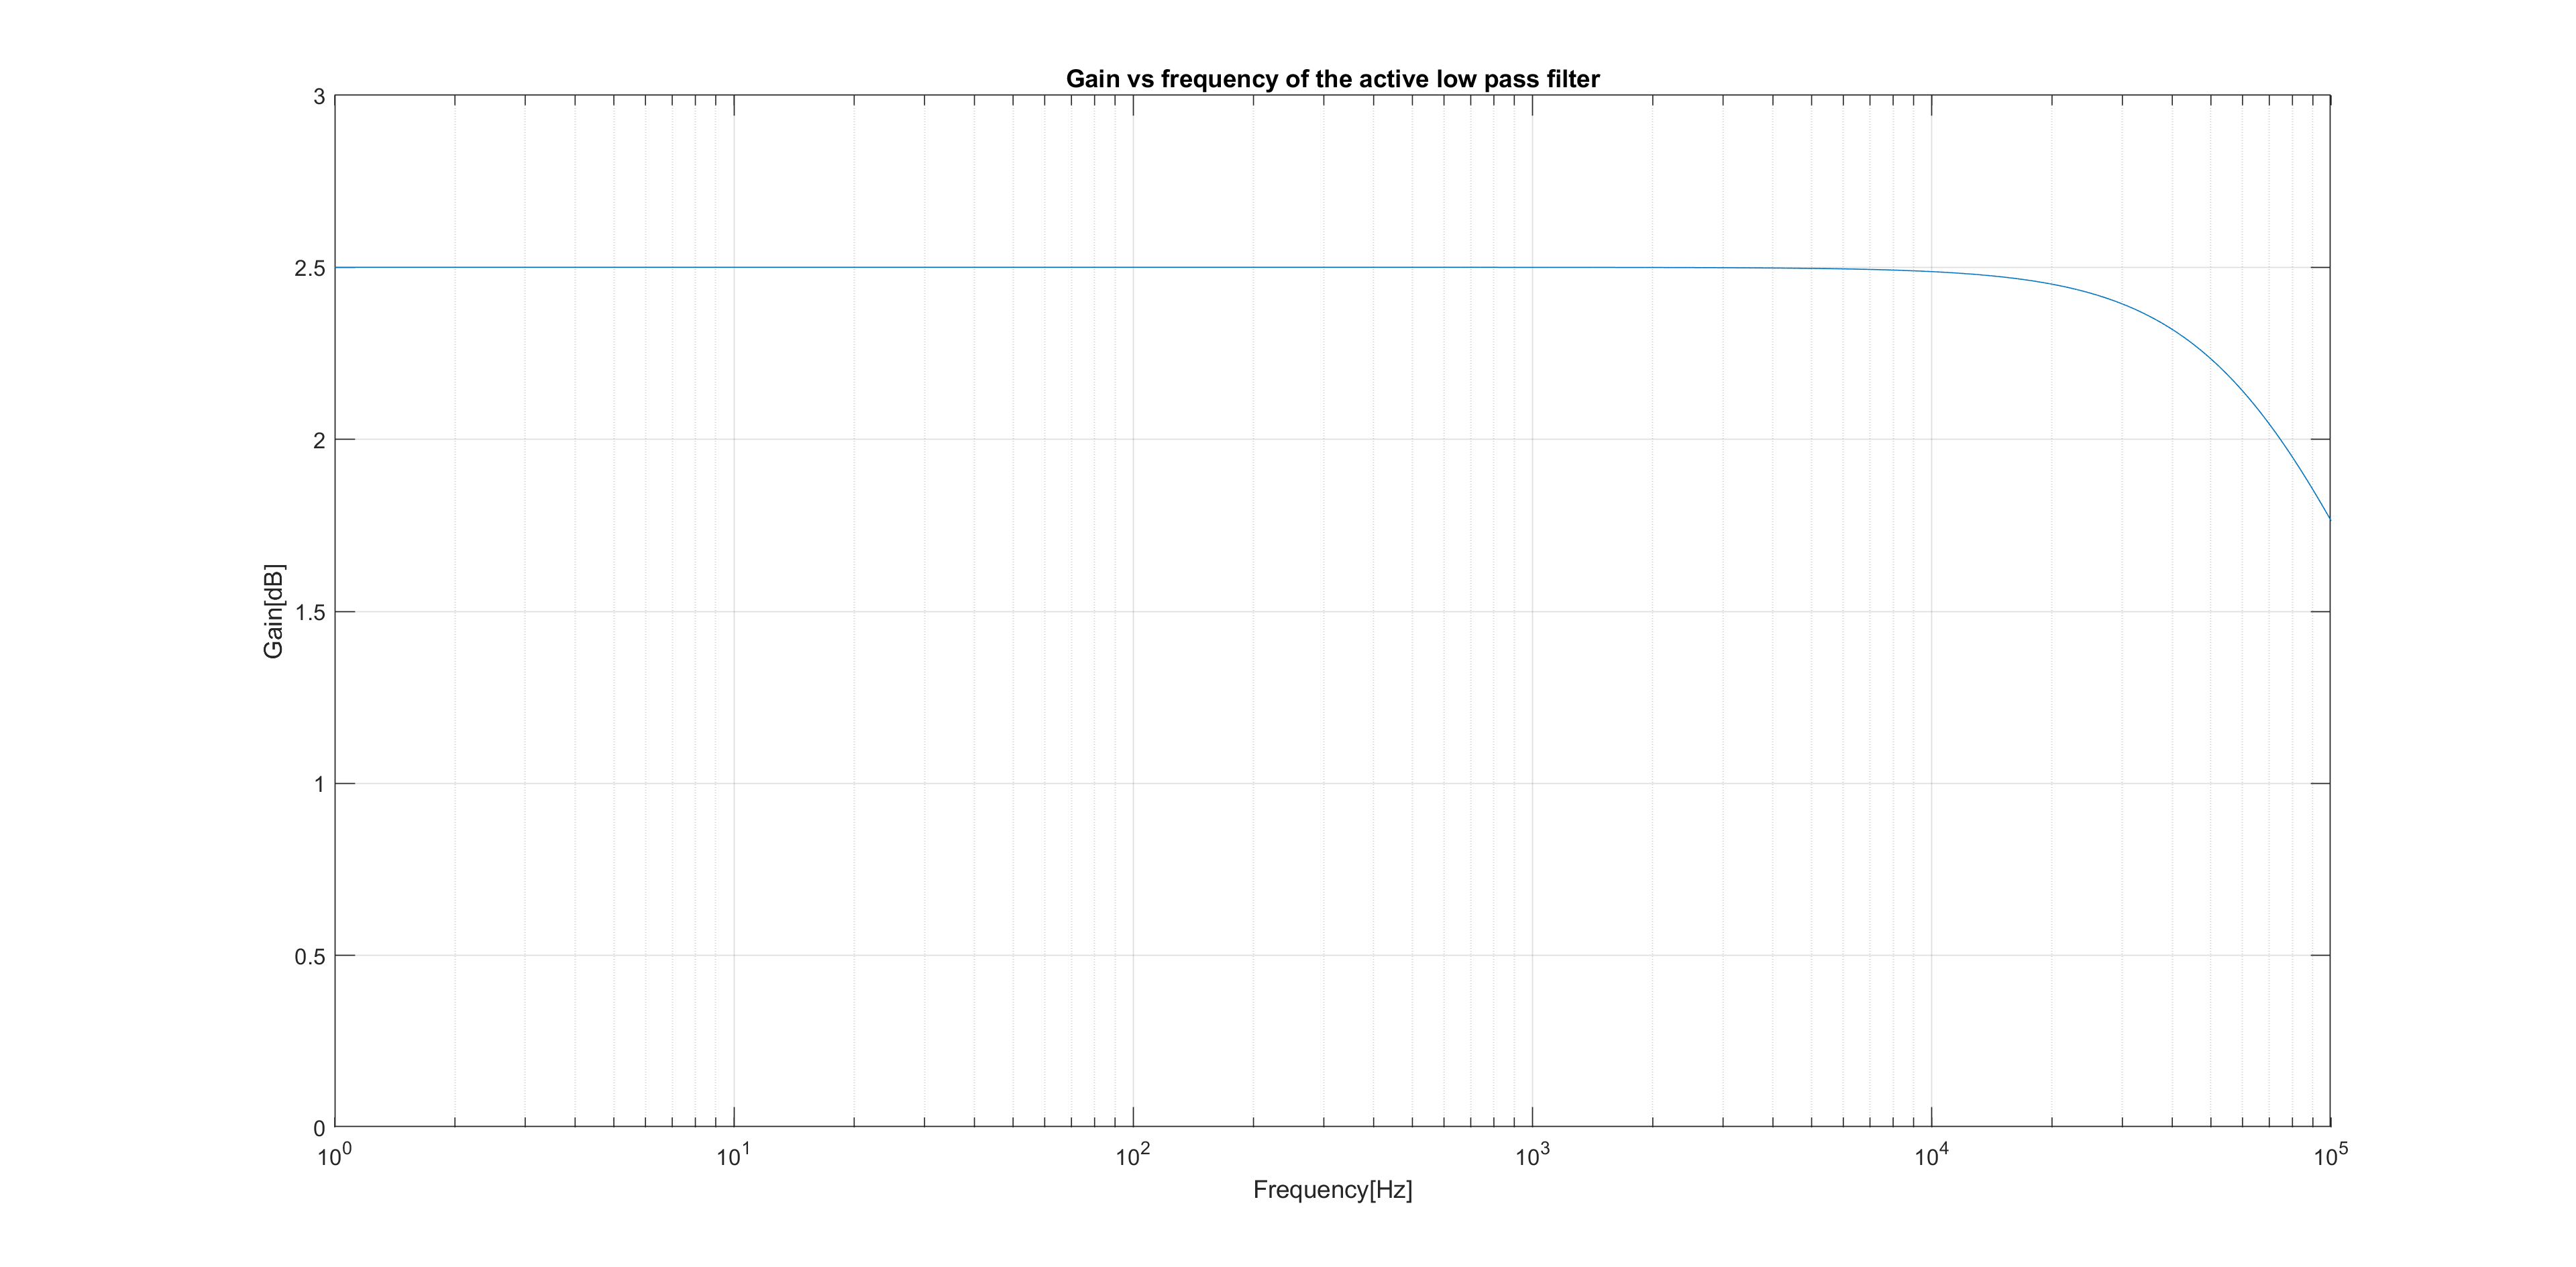
\includegraphics[width=0.7\textwidth]{graphics/Av_Lowpass.png}
    \caption{The gain of the operational amplifier with the active low pass filter.}
    \label{fig:AVlowpass}
\end{figure}

\textit{Figure~\ref{fig:Opamp3}} shows the scaling summing operational amplifier which is used to shift the input signal by 1.65Vdc. 


\begin{figure}[h]
    \centering
    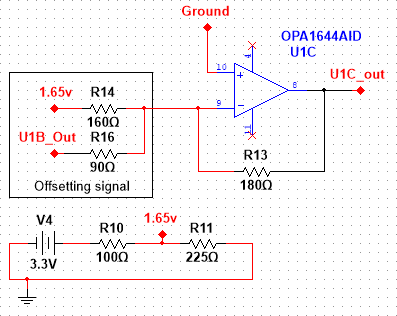
\includegraphics[width=0.70\textwidth]{graphics/OPamp3.png}
    \caption{The scaling summing operational amplifier, where the signal is shifted by 1.65Vdc}
    \label{fig:Opamp3}
\end{figure}


Which is important since the analog pins of the Teensy 3.5 have a voltage range of 0-3.3V.
There for the signal needs to be shifted by 3.3V/2 = 1.65Vdc.
%To estimate the voltage output of the op amplifier, \textit{Equation \ref{eq:invertDCGain}} and \textit{Equation \ref{eq:ScalingGain}} was used.
%For an input signal of 10mV amplitude, of the scaling summing op amp would be \textbf{KANSKI EKKI HAFA ?!?!?!} 
%$$V_{out} = -180\Omega(\frac{1.65V}{180\Omega} + \frac{\pm 10mV}{90\Omega}) = \pm $$
A voltage divider was needed to determine the resistor values for the 1.65Vdc which would ultimately put some design restraints on R16 and R13 seen in \textit{Figure~\ref{fig:Opamp3}}.
Firstly it was decided to have $R10 = 100\Omega$  and $R11 = 225\Omega$ to start off the calculations.
From that R14 could be calculated as $180\Omega$.
$$3.3V = \frac{\frac{1}{\frac{1}{180\Omega}+\frac{1}{225\Omega}}}{100\Omega+\frac{1}{\frac{1}{180\Omega}+\frac{1}{225\Omega}}} = 1.65V$$
Which was changed to $160\Omega$ because of the addition of R16 and using Multisim it was determined that $160\Omega$ would yield the closest results to the 1.65Vdc.
The gain for the input signal from the low pass filter is found by using \textit{Equation \ref{eq:invertDCGain}}
$$A_{V3} = -\frac{180\Omega}{90\Omega} = -2$$
The operational amplifier is in an inverting configuration which turns positive voltage signals to negative.
This needs to be rectified, since the Teensy 3.5 analog pins do not have a negative voltage range.
Which is done by another inverting operational amplifier, seen in \textit{Figure~\ref{fig:Opamp4}}.

\begin{figure}[h]
    \centering
    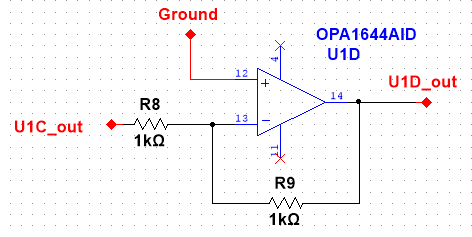
\includegraphics[width=0.70\textwidth]{graphics/OPamp4.png}
    \caption{The final operational amplifier, which is in an inverting configuration.}
    \label{fig:Opamp4}
\end{figure}

\fxfatal{Bæta við 330ohm viðnámi í Teensyinn}

The gain of inverting amplifier is found using \textit{Equation \ref{eq:invertDCGain}}.
$$ A_{V4} = -\frac{1k \Omega}{1k \Omega} = -1$$
The total circuit therefore consists of four operational amplifiers, high pass and low pass filter.
\textbf{MÖGULEGA BÆTA JÖFNU 'I KAFLA 2}
The total gain of the circuit for the input signal is found by.

$$A_{tot} = A_1A_1A_2A_3A_4 = 20*2.5*-2*-1 = 100$$

Finding the total dB gain of the circuit can be found by \textit{Equation \ref{eq:DBGAIN}}, which is confirmed using Multisim as seen in \textit{Figure~\ref{fig:bode}}.

$$dB = 20log(100) = 40dB$$


\begin{figure}[h]
    \centering
    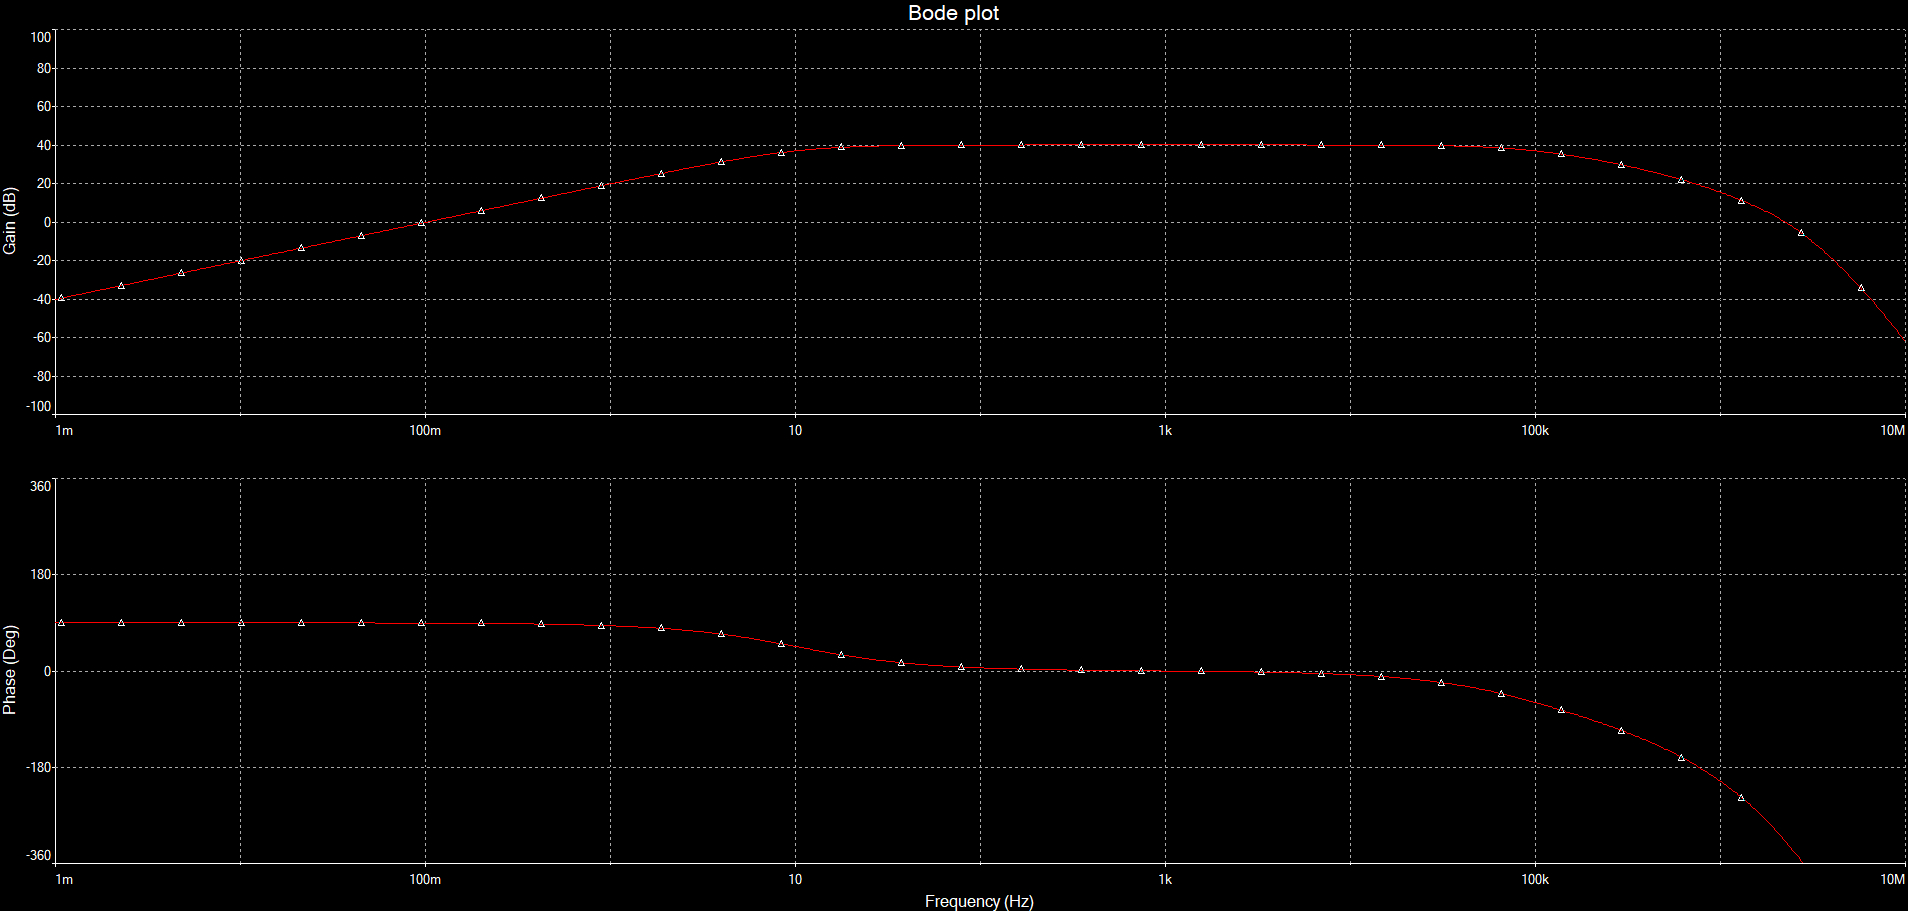
\includegraphics[width=1.0\textwidth]{graphics/bodeNew.png}
    \caption{The bode plot of the circuit.}
    \label{fig:bode}
\end{figure}



Several simulations of the circuit were performed in Multisim.
Which yielded the results seen in \textit{Figure~\ref{fig:InpVsOut10} -~\ref{fig:bode}}.
Using the setup of the circuit seen in \textit{Figures~\ref{fig:Opamp1}~\ref{fig:Opamp2}~\ref{fig:Opamp3}~\ref{fig:Opamp4}}. 
\textbf{LAGA MYNDIR EFTIR testinu}

\begin{figure}[h]
    \centering
    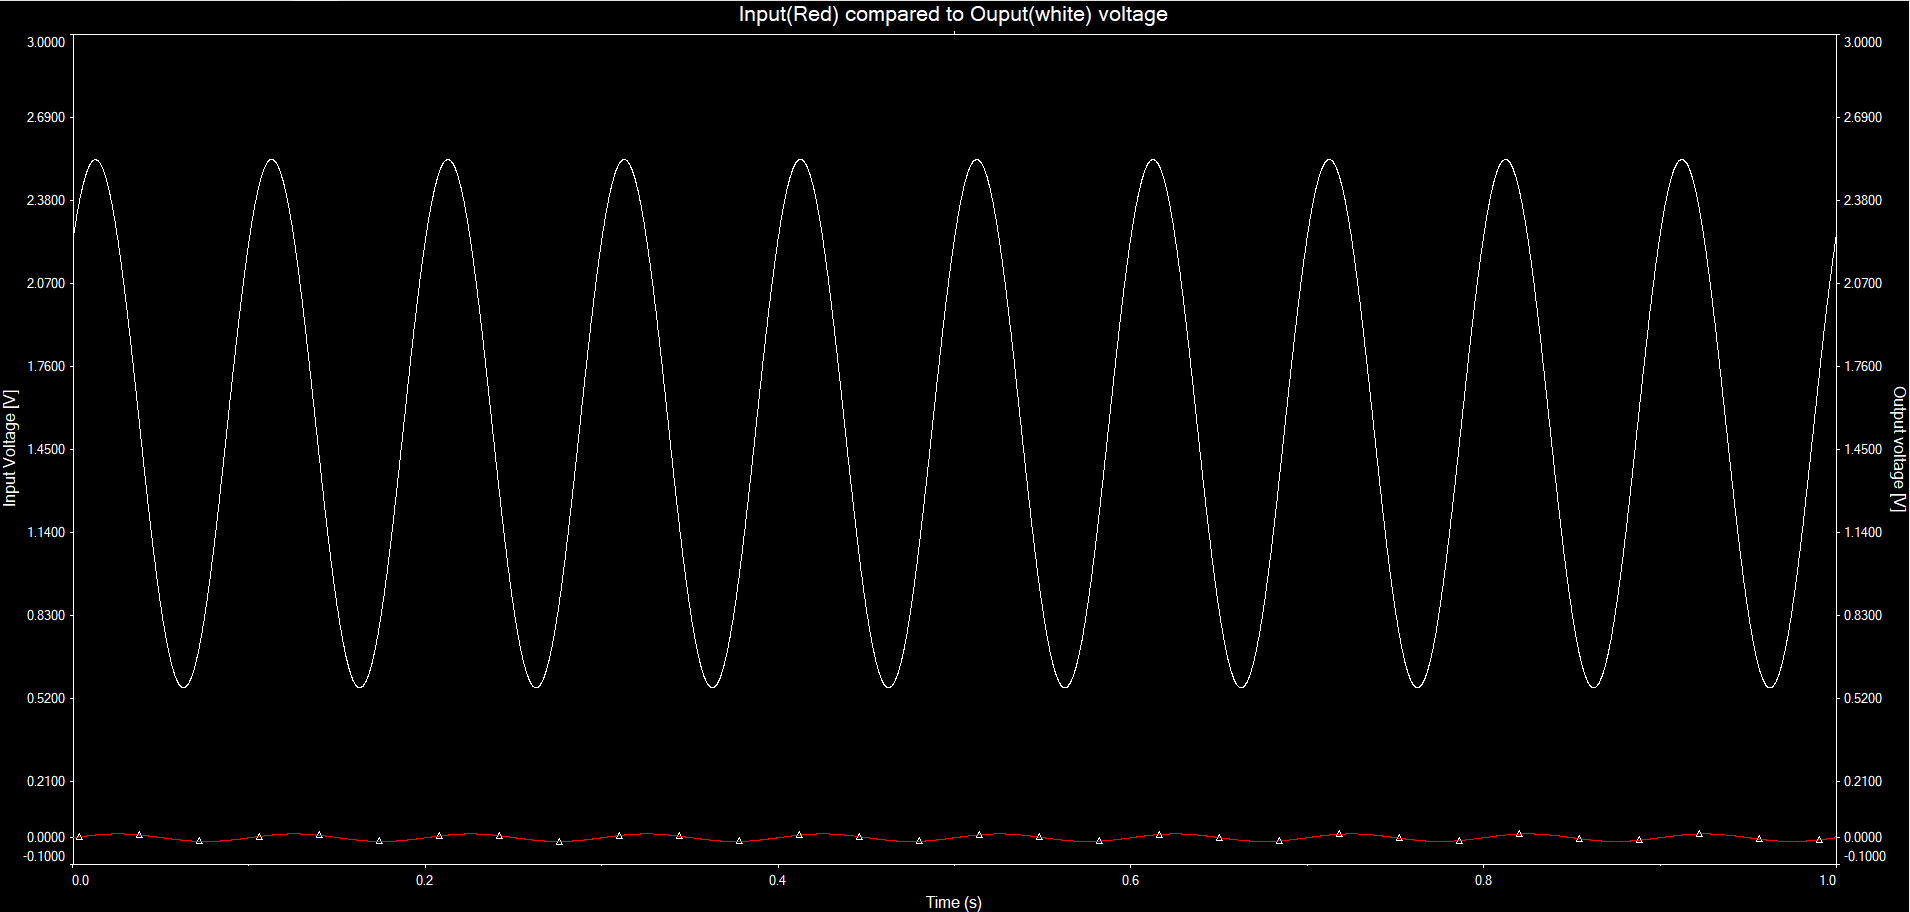
\includegraphics[width=1.0\textwidth]{graphics/InpVsOut10hz.png}
    \caption{With an input signal of 10mV RMS, at 10HZ.}
    \label{fig:InpVsOut10}
\end{figure}

The simulation was run using an AC voltage generator which was set to output 10mV RMS and 10Hz.
Which yielded the results seen in \textit{Figure~\ref{fig:InpVsOut10}}.
\textbf{TALA UM MEIRA}

\begin{figure}[h]
    \centering
    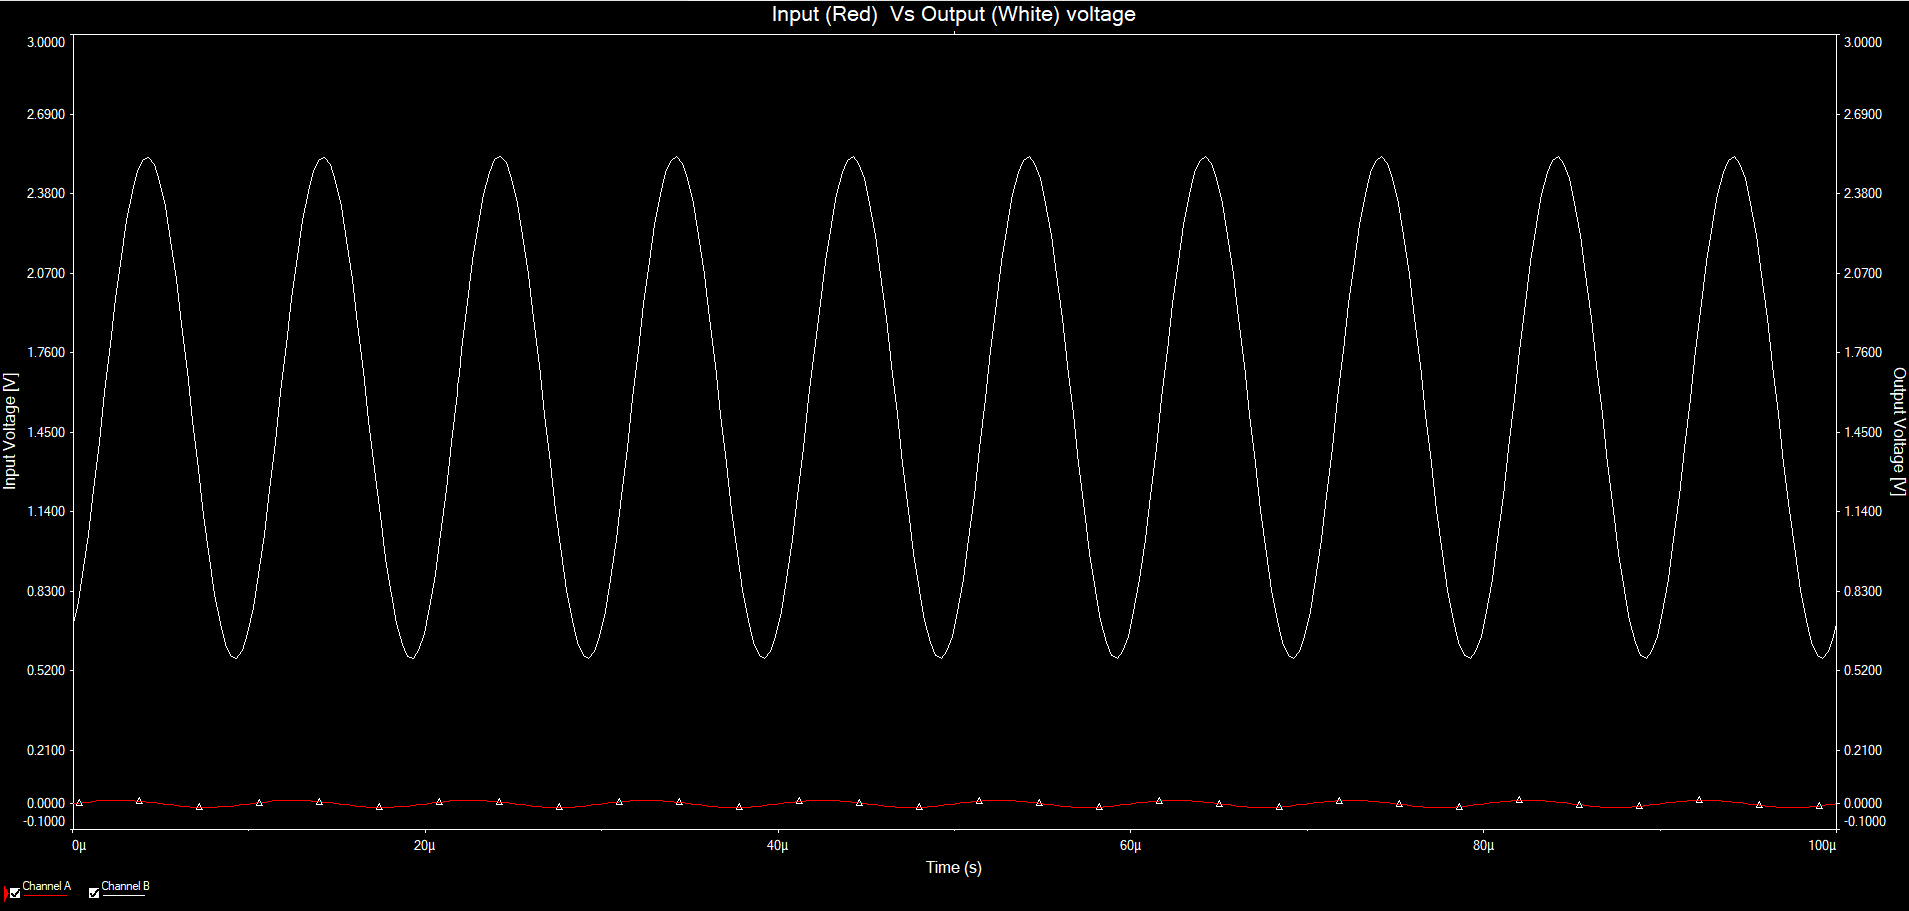
\includegraphics[width=1.0\textwidth]{graphics/InpVsOut100khz.png}
    \caption{With an input signal of 10mV RMS, at 100kHZ.}
    \label{fig:InpVsOut100k}
\end{figure}

\textbf{Bæta VIÐ 50khz multisim testi}

The simulation was run using an AC voltage generator which was set to output 10mV RMS and 100kHz.
Which yielded the results seen in \textit{Figure~\ref{fig:InpVsOut100k}}.
\textbf{TALA UM MEIRA}




The bode plot of the circuit can be seen in \textit{Figure~\ref{fig:bode}}.
It shows  circuit has a dB gain of $\approx$ 40, for the entire bandwidth of 10 - 100kHz.



\clearpage
\subsection{Code}


\textbf{BREYTA NÖFNUM}


All codes were developed in Arduino IDE using a teensyduino extension.
Since this project is about the data acquisition of cetacean vocalization, all codes were developed to read analog signal and write the value to a file on a SD card.
The SD card used was a Samsung EVO Plus microSDHC 32 GB, capable of 95MB/s read speed and 20MB/s write speed.
Which should be sufficient since the data is 2 bytes per sample which means in theory the card should be able to handle a peak of 10Msps.



\textbf{SKOÐAFYRIR UTERIKNGA Á CONVERSION T'IMA!!!!!!!!!!!!!!!!}
% https://www.pjrc.com/teensy/K64P144M120SF5RM.pdf bls 859

\subsubsection{ContinousAnalogRead}

The basic function of the code is simple, it should read a 64KB buffer of  analog values from the circuit as well as save the microseconds of each read in a different buffer.
Once the buffers are full, the program begins to write all the buffer to the SD card.
To configure the ADC the, the ADC library by pedvide was used \cite{villanueva_pedvideadc_2021}.
The library handles the configuration of the built-in ADC and should make that process easier, however it makes it a little harder to see what it exactly configures the ADC to be.
To use the library, the code must first create an ADC object via 
$ADC *adc = new ADC();$
which is then used to define the attributes of the ADC, which can be seen in lines 69 - 83 in~ \textit{Listing~\ref{src:ContAnalogRead}}. 
The reference voltage is set as 3.3V, to have a voltage range of 0 - 3.3V.
The ADC averaging is set to 0, which after testing was the fastest configuration.
The conversion speed of the ADC was set to the fastest setting for 16bits conversion or HIGH\_SPEED\_16BITS, which sets the ADC clock to $<= 12 MHz$.
Then the sampling speed was set to the fastest setting of VERY\_HIGH\_SPEED, which adds +0 cycles to ADC clock (ADCK).
The library can as well configure so that once a conversion occurs an isr is triggered which is done by the enable interrupts function, and ties the conversion of adc0 to void adc0\_isr.
To set the ADC to do a continuous conversion, startContinuous() is used and can be configured to a specific pin on the Teensy.
Finally the results of the conversion are found using analogReadContinuous().

Once the ADC is configured, the device can start reading analog values.
It collects the analog readings to a buffer as well as the timestamp of each reading.
Once the buffers are full, the program writes to a SD card.
It writes both values as decimal values to a text file on the card.
The analog read and writes to SD card can be seen in \textit{Figure~\ref{fig:ContAnalSpeed}}

\begin{figure}[h]
    \centering
    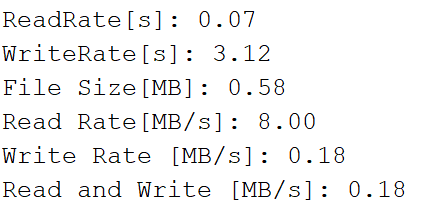
\includegraphics[width=0.50\textwidth]{graphics/ContinousReadSpeed.png}
    \caption{The read and write speeds of ContinuousAnalogRead.ino}
    \label{fig:ContAnalSpeed}
\end{figure}


The data recorded by the device with the ContinuousAnalogRead.ino as the code. 
With an input signal of 10mVpp and 50kHz frequency. 
It appears to run too fast for the ADC, seeing as it has several conversions made at each voltage level as seen in \textit{Figure~\ref{fig:ContAnalREsults}}, every three data point a new conversion occurs.
Even though it should wait until the ADC is ready for a new conversion it does not appear to do so.


\begin{figure}[h]
    \centering
    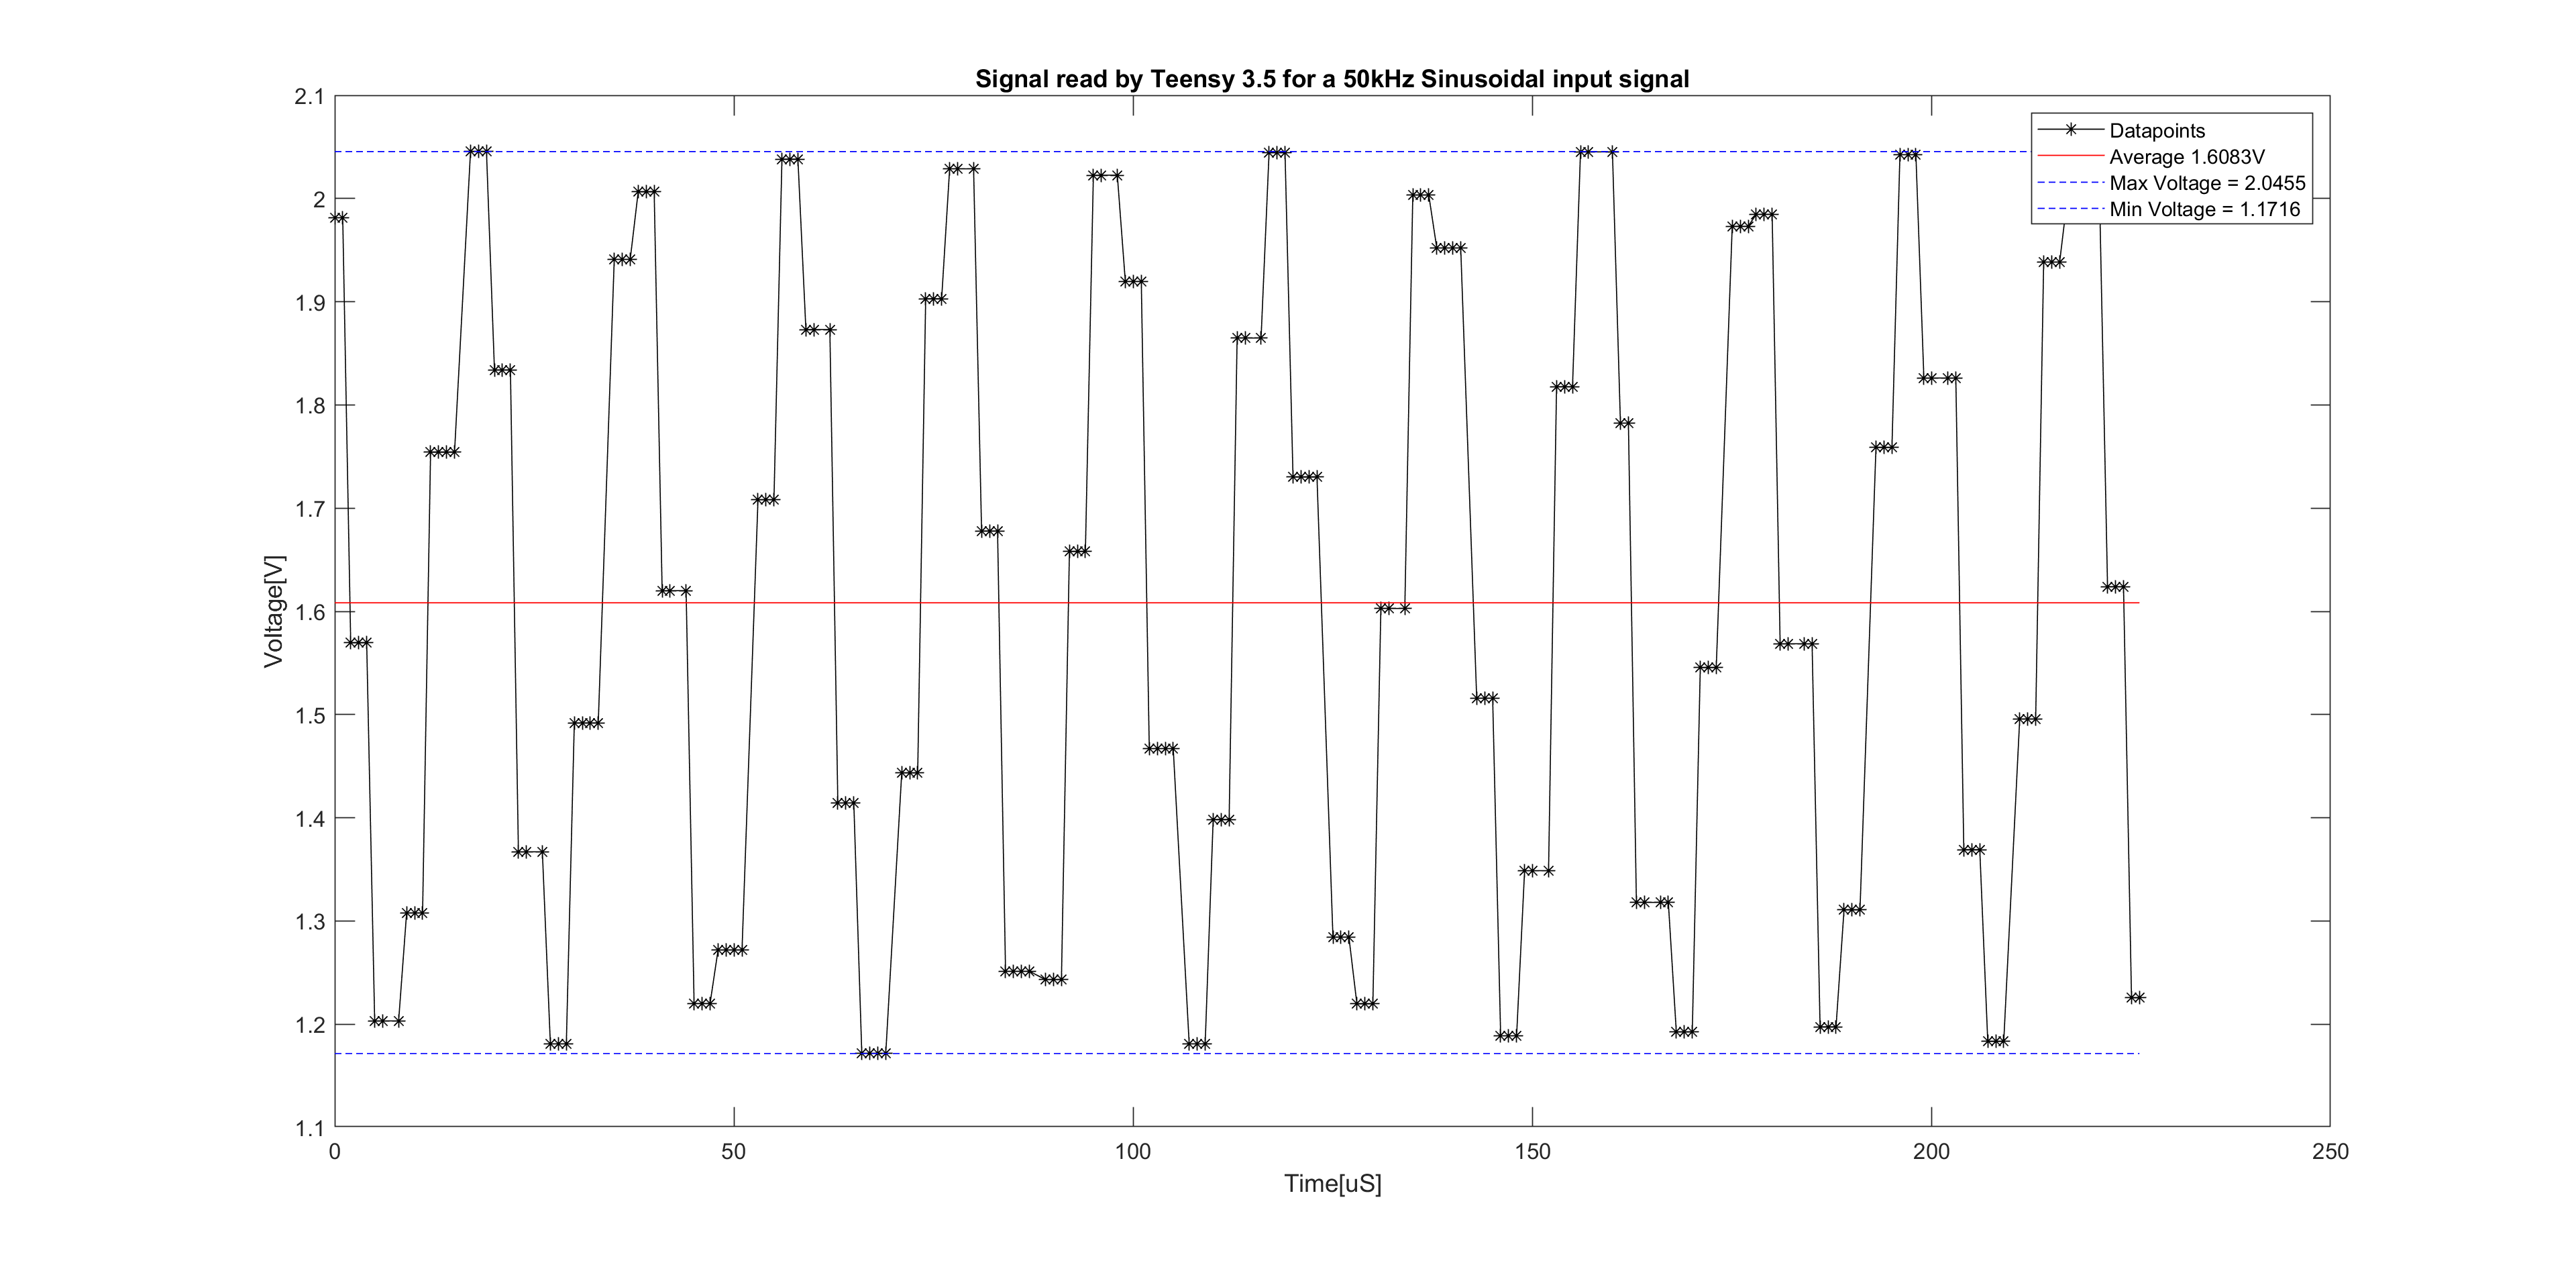
\includegraphics[width=1.0\textwidth]{graphics/COntANalogResults.png}
    \caption{Results from Teensy using ContinuousAnalogRead.ino.}
    \label{fig:ContAnalREsults}
\end{figure}

Just before the test a single reading of the output signal was taken with an oscilloscope which can be seen in \textit{Figure~\ref{fig:ContAnalOscillascope}}.

\begin{figure}[h]
    \centering
    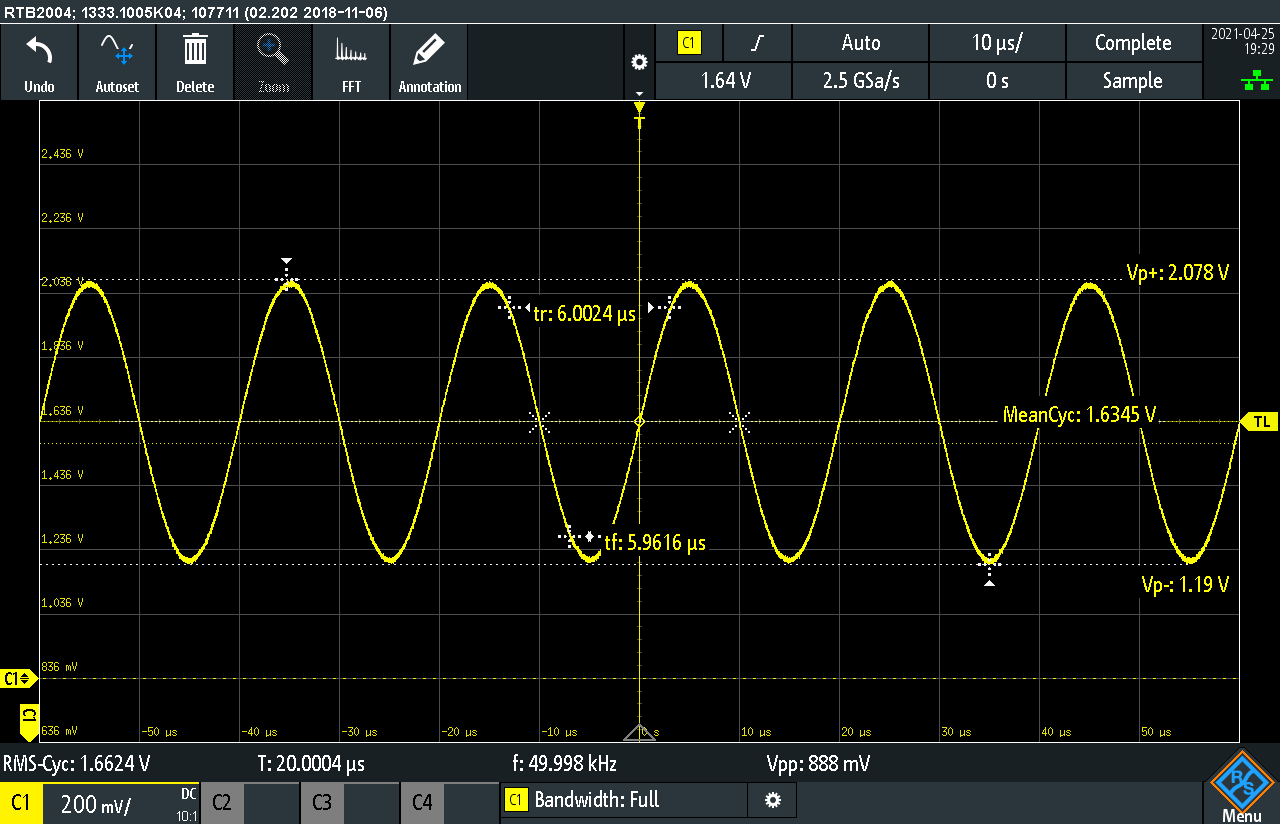
\includegraphics[width=0.70\textwidth]{graphics/ContAnalogReadOscillascope.PNG}
    \caption{Oscilloscope readings of the output signal}
    \label{fig:ContAnalOscillascope}
\end{figure}

%\begin{figure}[h]
%    \subfloat[\textbf{Sub figure caption}]{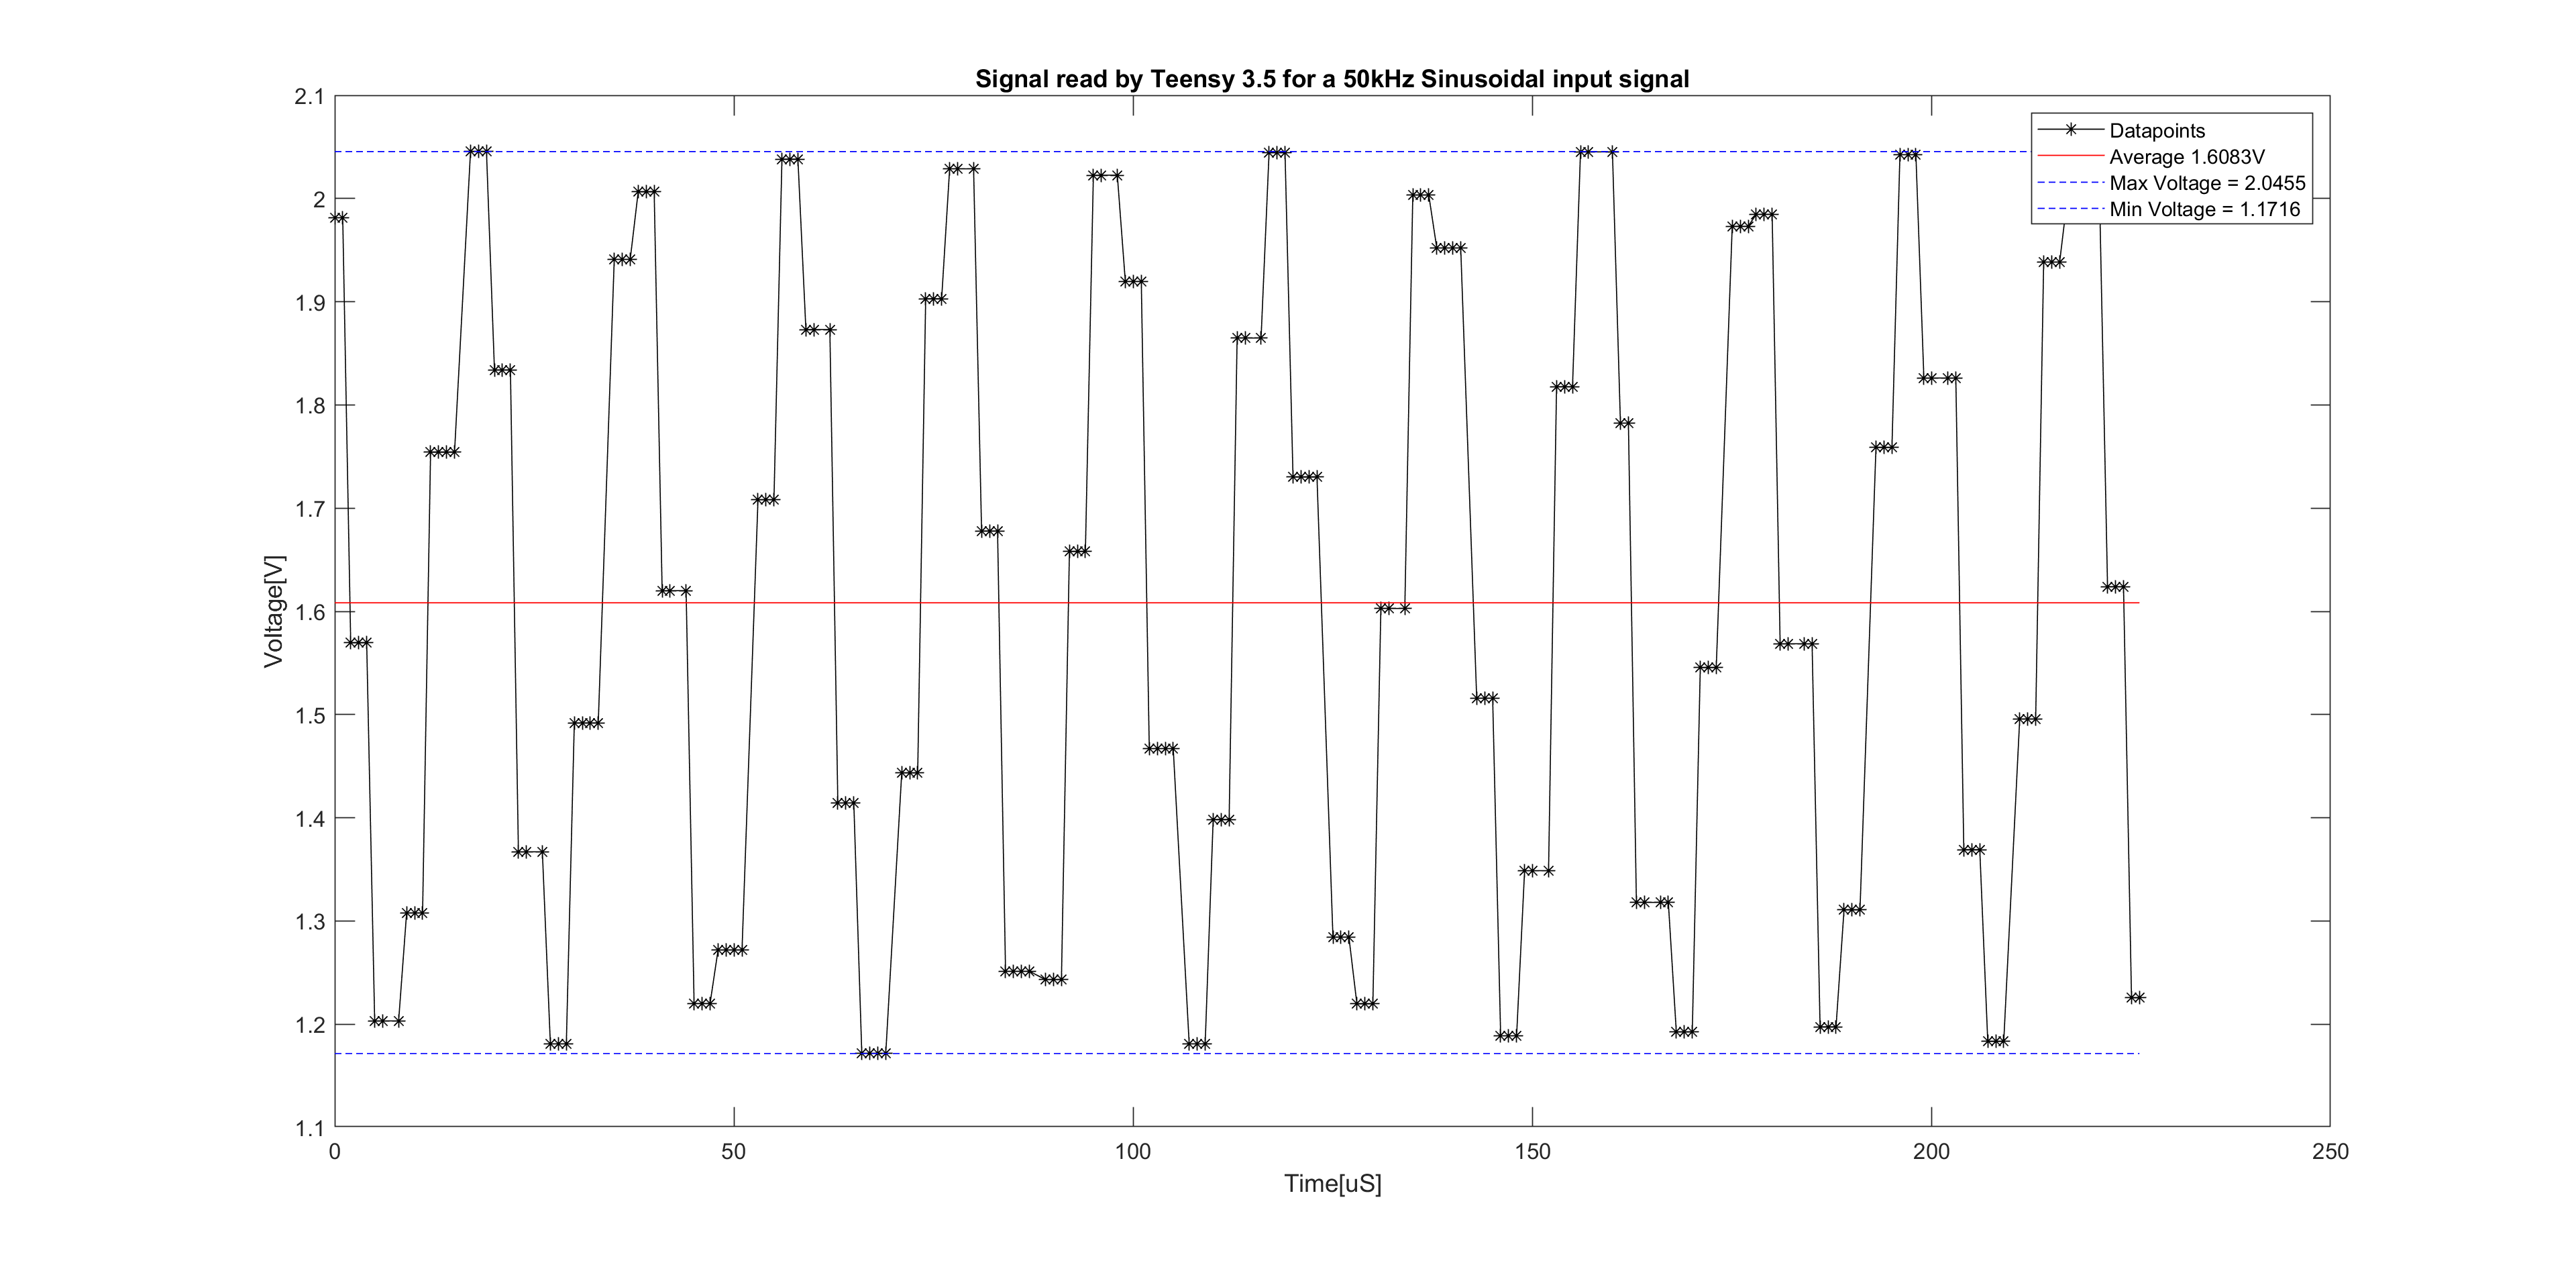
\includegraphics[width=0.50\textwidth,height=0.40\textwidth]{graphics/COntANalogResults.png}}
%    \label{fig:ContAnalSpeedREsults}
%    \hfill
%    \subfloat[\textbf{Sub figure caption }]{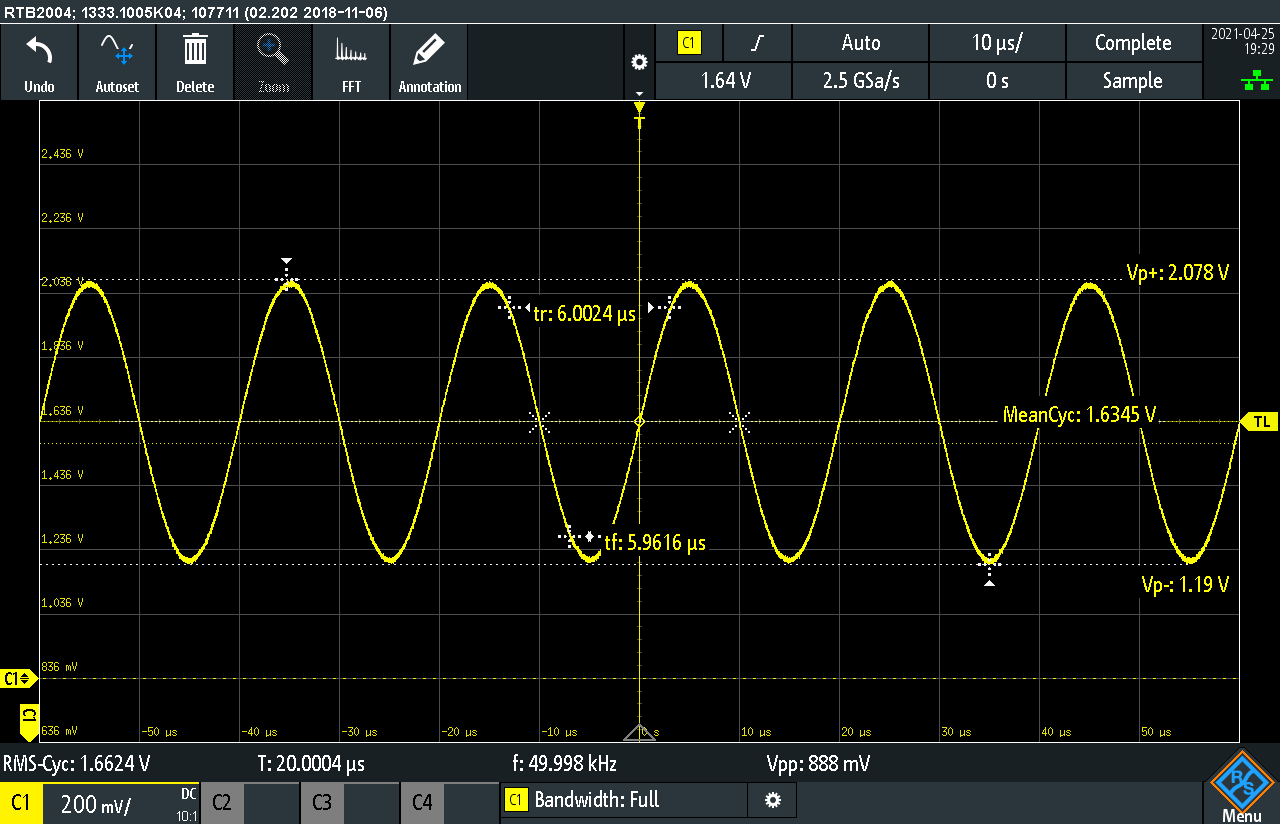
\includegraphics[width=0.40\textwidth,height=0.40\textwidth]{graphics/ContAnalogReadOscillascope.PNG}}
%    \label{fig:ContAnalOscillascope}
%    \caption{Results from the device compared to the oscilloscope readings}
%%\end{figure}


\subsubsection{PDBtestest}

\textbf{Bæta við meiri lýsingu á mannamáli og kanski pseudo kóða}

\textbf{PDBtestest} utilizes three specific builtin peripherals on the Teensy3.5 in order to read analog signals, which are an ADC, a programmable delay block (PDB) and a DMA channel.
The PDB is an accurate timer that is used to trigger the ADC to do a analog to digital conversion.
Once each ADC conversion is complete DMA receives a trigger, the ADC value is then transferred using DMA to memory.
When initializing the DMA it needs to know a few things about the buffer to which the ADC value is being transferred to such as the size of the buffer and its address. 
This is important because DMA counts how many transfers have been made, and at a set number of transfers it triggers an ISR.
Since in this program the DMA buffer is a 2 dimensional array (2 by 256 to have each buffer 512 bytes in size).
The ISR is set to trigger when each of the buffer is full, meaning when the first buffer is full the ISR is triggered and its contents are moved to another storage buffer.
While that transfer is happening the destination address for the buffer was changed to the second buffer and the data transfer is continually happening while the first buffer is still transferring its contents to the storage buffer.
This is crucial in order to get a non blocking code and not loose any data.
Therefor the speed of the program is dependent on how fast the Teensy can move data from the DMA buffer to the storage buffer.
The main program is then continually writing from the storage buffer to the SD card is 512 byte chunks.

\begin{figure}[h]
    \centering
    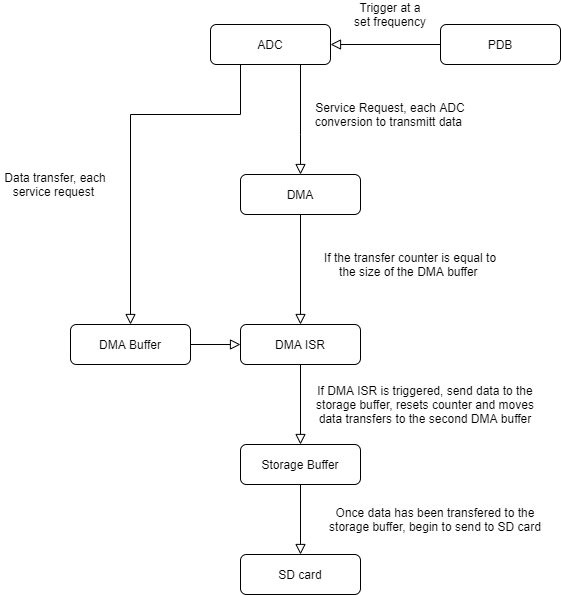
\includegraphics[width=0.70\textwidth]{graphics/flowChart.png}
    \caption{A flow chart giving a visual representation of the function of the program}
    \label{fig:CodeFlow}
\end{figure}



\subsection{Testing}



Skoða aftur á scopei færa langt frá trigger punknt ~50 sveiflur og skoða breytileika þar.
skða líka með FFT
Skoða með mismunandi söfnunartíðnum og bera saman og skoða powerið

skoða innmerki  10k með 100k söfnunartíðni
                20k með 200k söfnunartíðni
                30k með 300k söfnunartíðni

Hvað ég safna rétt í tíma
hve mikið hljóð
setja inn merki, mæla útmerkið með FFT á scopei.
skoða hljóð frá generatornum og svo frá merkinu með fft
sjá mynd, ef það koma eh suð toppar á fft frá bara generator, sjá hvort þeir detta niður með RC filter ef ekki þá er suðið að koma frá kerfinu.



%\textbf{looking at the oscilloscope on the builtin led, triggering it to switch states each time ISR of individual peripheral is %triggered. 
%Changing ISR only pdb = stable till sampleFreq  roughly 1MH  (491.7kHz)+- 0.3kHz measured by scope
%for 16 bits:
%ISR pdb adc = stable till sampleFreq roughly 280kHz   (139.5kHz) +- 0.01kHz measured by scope
%whole system = stable till roguhly 300khz samplefreq 
%Changing the resolution had minimal gains.
%It seemed to be able to be triggered a little bit faster however those were not stable for the teensy and the program would crash.}


Equipment used for tests can be seen in the list below.
\begin{itemize}
    \item \textit{Rhode \& Schwarz RTB20004} digital oscilloscope with a 2.5 Gsps sampling rate for wave form confirmation.
    \item \textit{Rigol DG1022} wave form generator capable of generating signals upto 25MHz sine wave and a resolution of 1$\mu Hz$ and down to 2mVpp.
    \item \textit{Rigol DP831} programmable DC power supply.
\end{itemize}



\subsubsection{Frequency of PDB, ADC and the DMA}

Several tests were made in order to find the maximum frequency at which parts of the device could remain relatively stable.
These tests would use an ISR, triggered by either the PDB or the ADC.
The ISR would either turn on the buildin LED on the Teensy or turn it off, depending on the whether the LED was on or off.
Which for every other trigger would make the LED blink.
Three test cases were examined, first using just the PDB which would trigger the ISR. 
Secondly the PDB and ADC together and finally for when the entire system was operational, for both cases the ISR would be triggered by the end of a ADC conversion.
The setup of the test can be seen in \textit{Figure~\ref{fig:SetupCircSpeed}}, the oscilloscope was connected to the builtin LED and the Teensy3.5 was powered via USB and the op amps were powered by the DC power supply.
The scope was set to take measurements of the time and frequency between the rising edge of rectangular signal that formed from blinking the LED. 
The oscilloscope shows the mean, maximum and minimum values for both, which are actually halved since the scope counts the rising edge of the pulses.
As well as the cursor was set over a single pulse to show the actual frequency of the ISR trigger speed.
The device was stopped when the oscilloscope had made roughly 10k wave count.
The setup was the same for all three test cases.

\fxfatal{Taka betri mynd}

\begin{figure}[h]
    \centering
    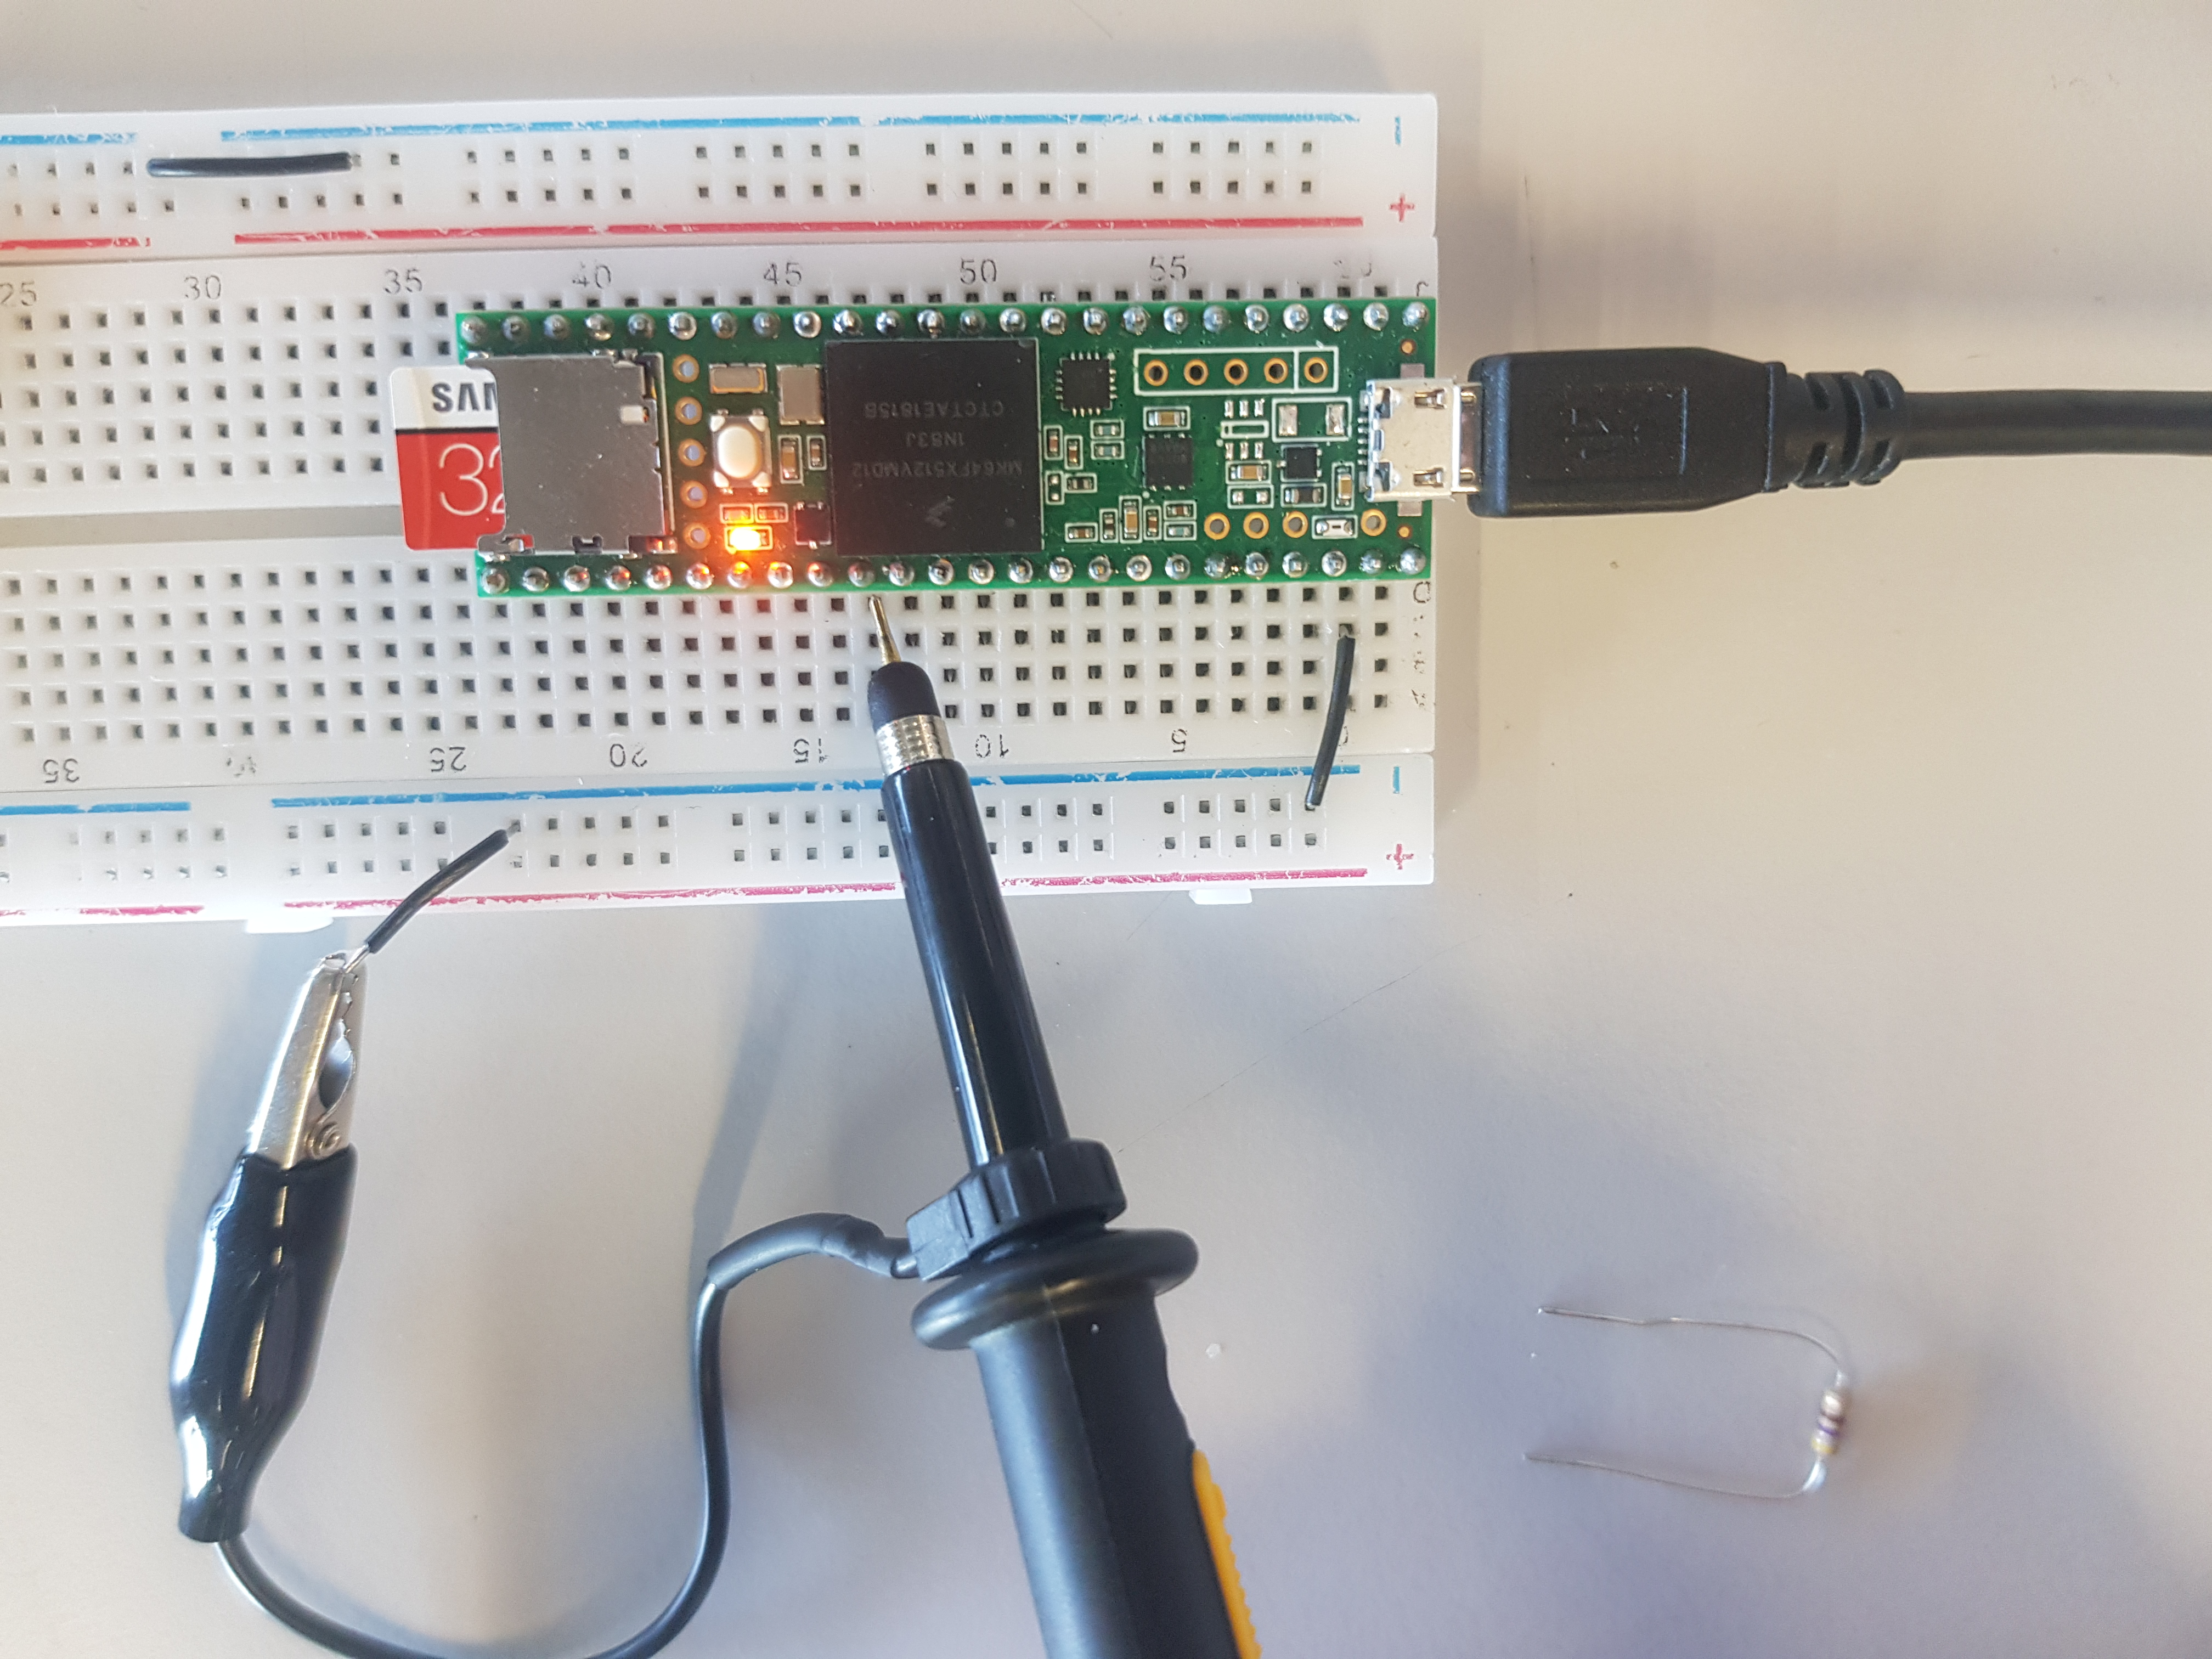
\includegraphics[width=0.7\textwidth]{graphics/SetupCircSpeed.jpg}
    \caption{The setup of the circuit for frequency for three test first just initializing the PDB, then the PDB and ADC and the third where the whole system was initialized.}
    \label{fig:SetupCircSpeed}
\end{figure}

In the first test, just the PDB timer was initialised and the ISR would trigger from the PDB timer.
Three set frequencies were tested, 1.2MHz, 600kHz and 300kHz.
The results of the tests can be seen in \textit{Figures~\ref{fig:PDBSp1200} - \ref{fig:PDBsp300}}.
The maximum frequency at which the PDB could run at was when the set frequency was set as 1.2MHz.
As explained before the actual frequency values from the oscilloscope are halved from the real values, so all measured frequency statistics are doubled, while the time of the period is halved.
The mean frequency was 1.17MHz, were the maximum was 1.27MHz and minimum of 767.7kHz with a standard deviation of 27.1kHz. 
The mean time for a period was 852ns with a standard deviation of 27ns as seen in \textit{Figure~\ref{fig:PDBSp1200}}.

\begin{figure}[h]
    \centering
    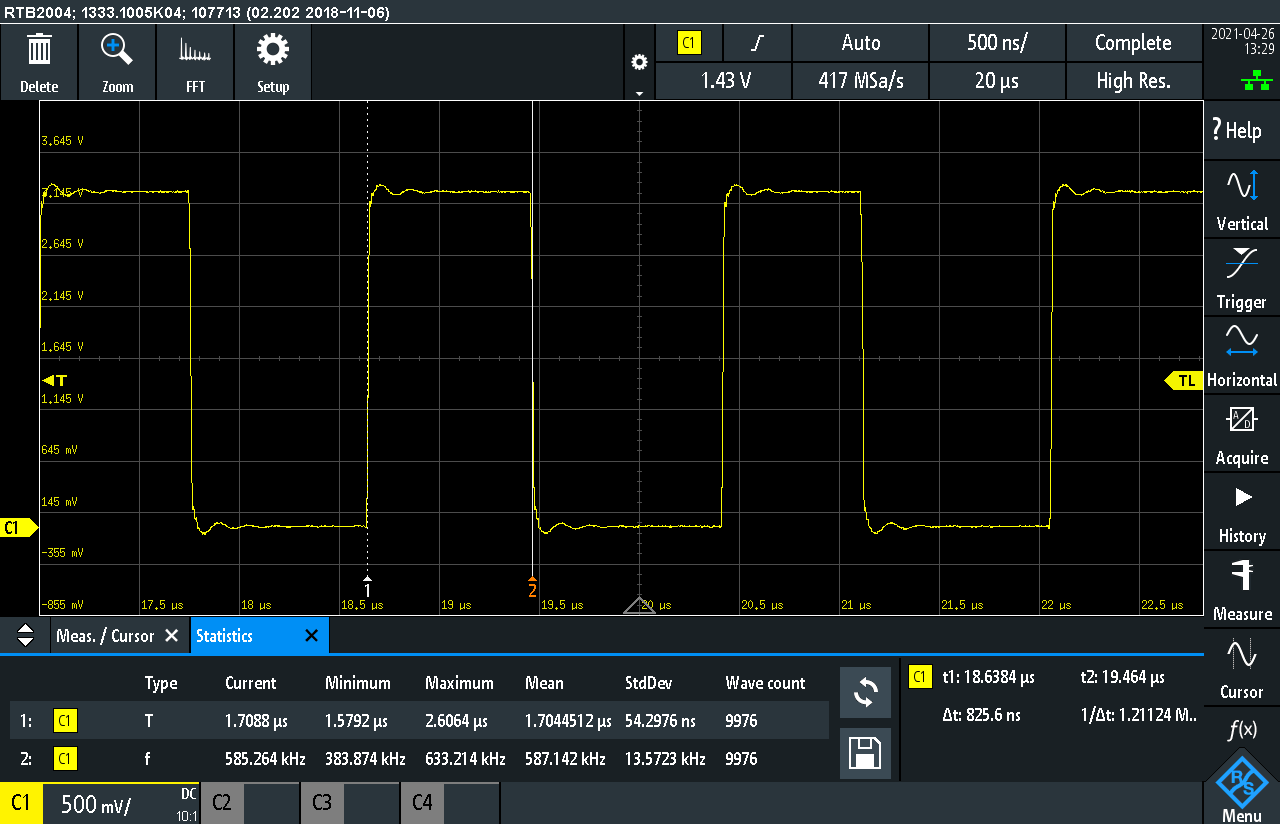
\includegraphics[width=0.8\textwidth]{graphics/STAT01_1200.PNG}
    \caption{The blinking of the LED, set frequency in the code was 1.2MHz}
    \label{fig:PDBSp1200}
\end{figure}

For the second test, the set frequency was 600kHz.
The mean frequency was 593.5kHz, were the maximum was 654.5kHz and minimum of 470.7kHz with a standard deviation of 8.42kHz. 
The mean time for a period was 1.68$\mu$s with a standard deviation of 29ns as seen in \textit{Figure~\ref{fig:PDBSp600}}.

\begin{figure}[h]
    \centering
    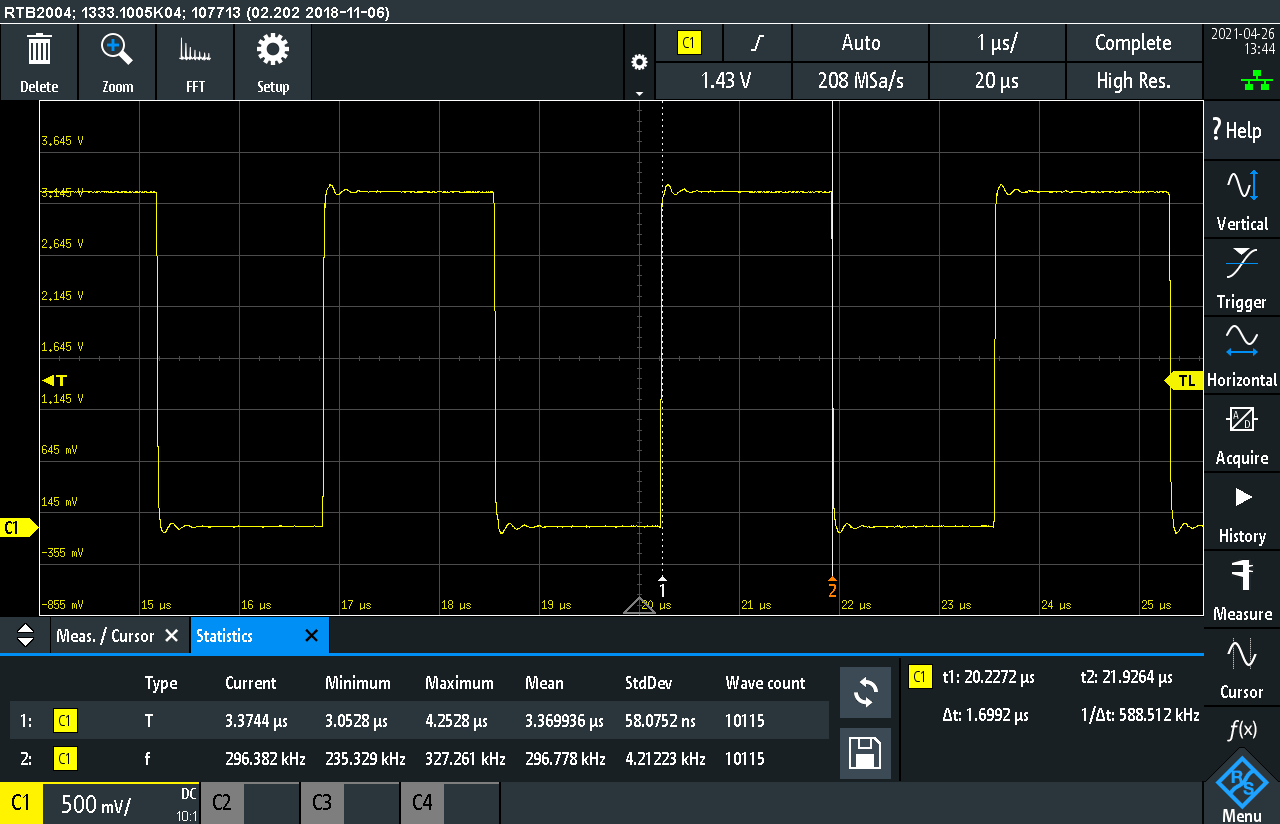
\includegraphics[width=0.8\textwidth]{graphics/STAT02_600.PNG}
    \caption{The blinking of the LED, set frequency in the code was 600kHz}
    \label{fig:PDBSp600}
\end{figure}

For the third test, the set frequency was 300kHz.
The mean frequency was 298.4kHz, were the maximum was 320.7kHz and minimum of 122.4kHz with a standard deviation of 1.63kHz. 
The mean time for a period was 3.35$\mu$s with a standard deviation of 21ns as seen in \textit{Figure~\ref{fig:PDBsp300}}.

\begin{figure}[h]
    \centering
    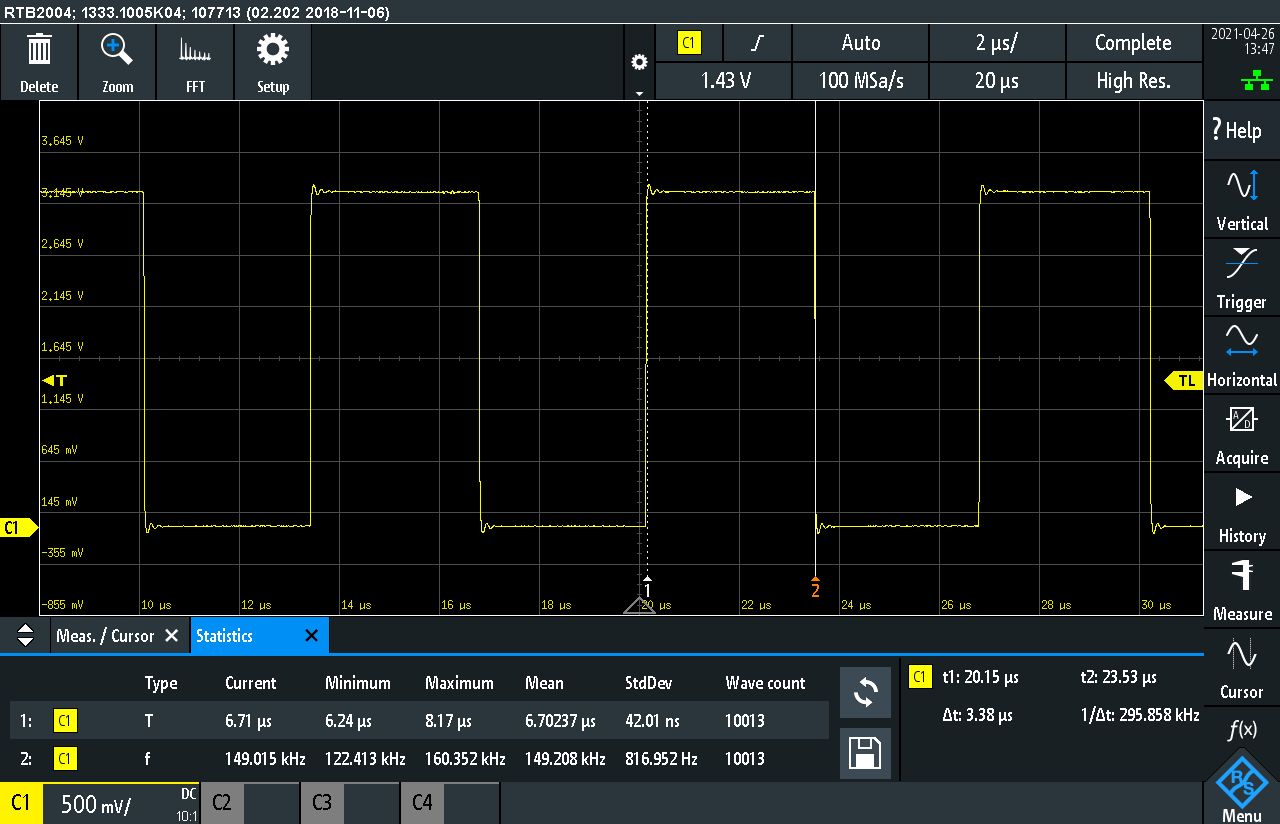
\includegraphics[width=0.8\textwidth]{graphics/STAT03_300.PNG}
    \caption{The blinking of the LED, set frequency in the code was 300kHz}
    \label{fig:PDBsp300}
\end{figure}

The next test was for the ADC, but now by initializing both the ADC and the PDB.
The ISR would also be set to trigger when completing an ADC conversion.
The set frequency was 280kHz, because at 300kHz the program would stop running after roughly 2 seconds.
The mean frequency was 279.1kHz, were the maximum was 208.3kHz and  minimum of 225.5kHz with a standard deviation of 1.1kHz. 
The mean time for a period was 3.58$\mu$s with a standard deviation of 14ns as seen in \textit{Figure~\ref{fig:PDBADCDMAsp280}}.

\begin{figure}[h]
    \centering
    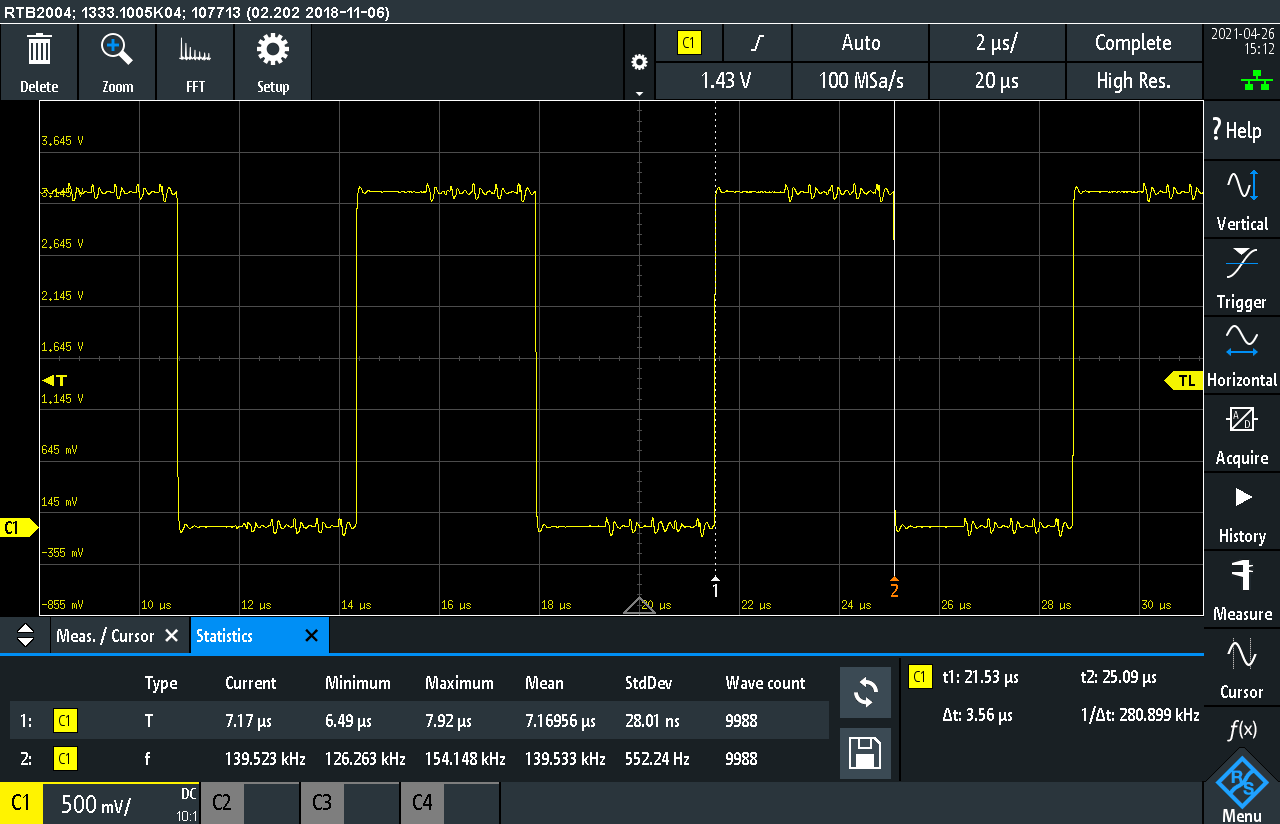
\includegraphics[width=0.8\textwidth]{graphics/STATADC_280.PNG}
    \caption{The blinking of the LED when completing an ADC conversion triggered the ISR, set frequency in the code was 280kHz}
    \label{fig:PDBADCDMAsp280}
\end{figure}

The next test was for the whole system was initialized.
The ISR is still set to trigger when completing an ADC conversion.
The mean frequency was 298.3kHz, were the maximum was 532.4kHz and minimum of 208.5kHz with a standard deviation of 5.4kHz. 
The mean time for a period was 3.39$\mu$s with a standard deviation of 69.6ns as seen in \textit{Figure~\ref{fig:PDBADCDMAsp280}}.

\begin{figure}[h]
    \centering
    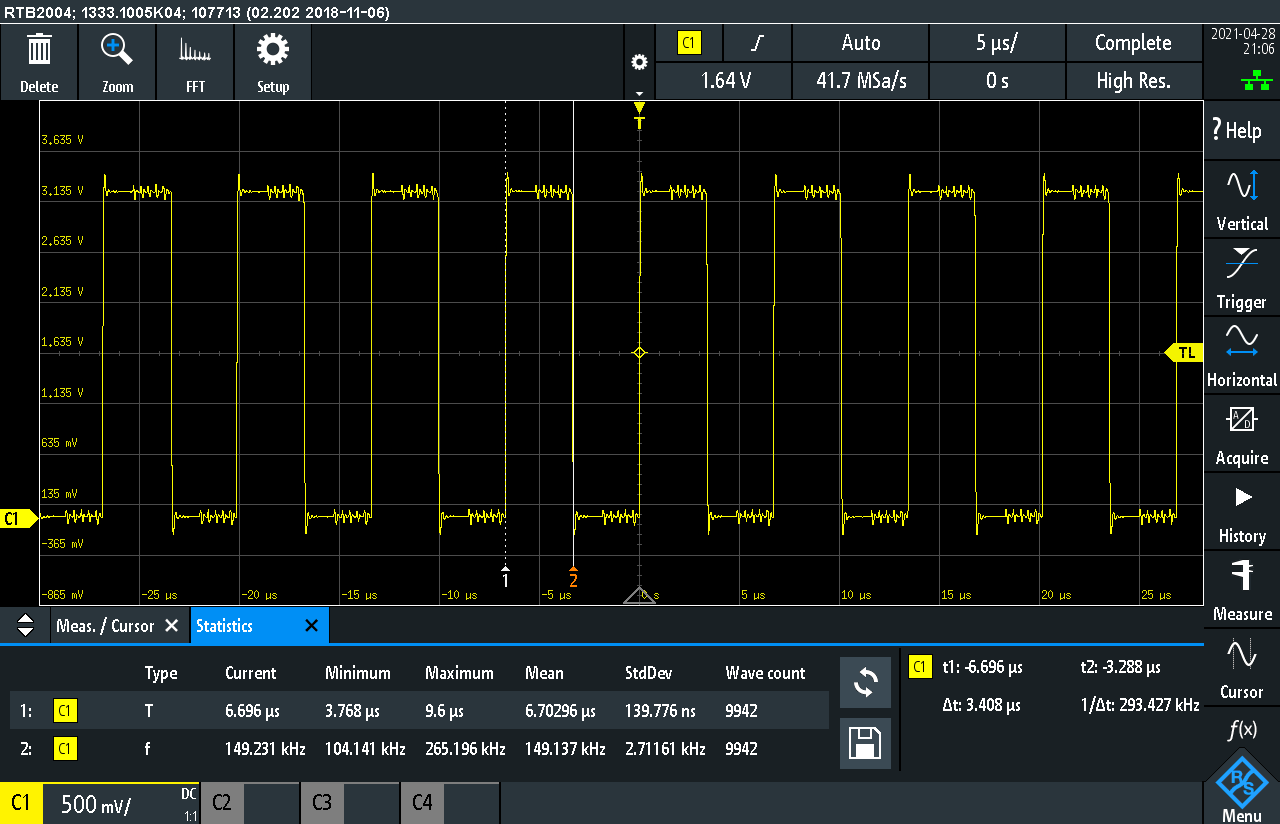
\includegraphics[width=0.8\textwidth]{graphics/ALLT300k.PNG}
    \caption{The blinking of the LED when completing an ADC conversion triggered the ISR, set frequency in the code was 300kHz}
    \label{fig:PDBADCDMAsp300}
\end{figure}


\clearpage




\subsubsection{Noise testing}

%setting https://picture.iczhiku.com/resource/eetop/SHkHEFiIIDHlSccB.pdf

Several tests were made in order to estimate the noise of the device.
Fast Fourier transform (FFT) function of the RTB2004 oscilloscope was used for the measurements and the DC power supply was used to power the op amps.
The oscilloscope was set to AC coupled for the best broadband range measurement%https://training.ti.com/ti-precision-labs-op-amps-noise-measuring-system-noise 
, attenuator set to 1:1 ratio %https://www.testandmeasurementtips.com/reduce-oscilloscope-noise-measurements/
for accurate noise measurements and the Hannig window was used for 
Two test cases where examined, first when a sine wave was the input of the circuit and secondly when the input was connected to ground.
For both cases the probe was connected to the output of the op amps.
The setup for the tests can be seen in \textit{Figure~\ref{fig:SetupFFT}}.

\textbf{%https://web.sonoma.edu/esee/courses/ee442/archives/sp2019/supp/defining_dBu.pdf
- skoða} 
%https://www.youtube.com/watch?v=oLBGNC9FGwo&ab_channel=TexasInstruments minuta 3:47

\begin{figure}[h]
    \centering
    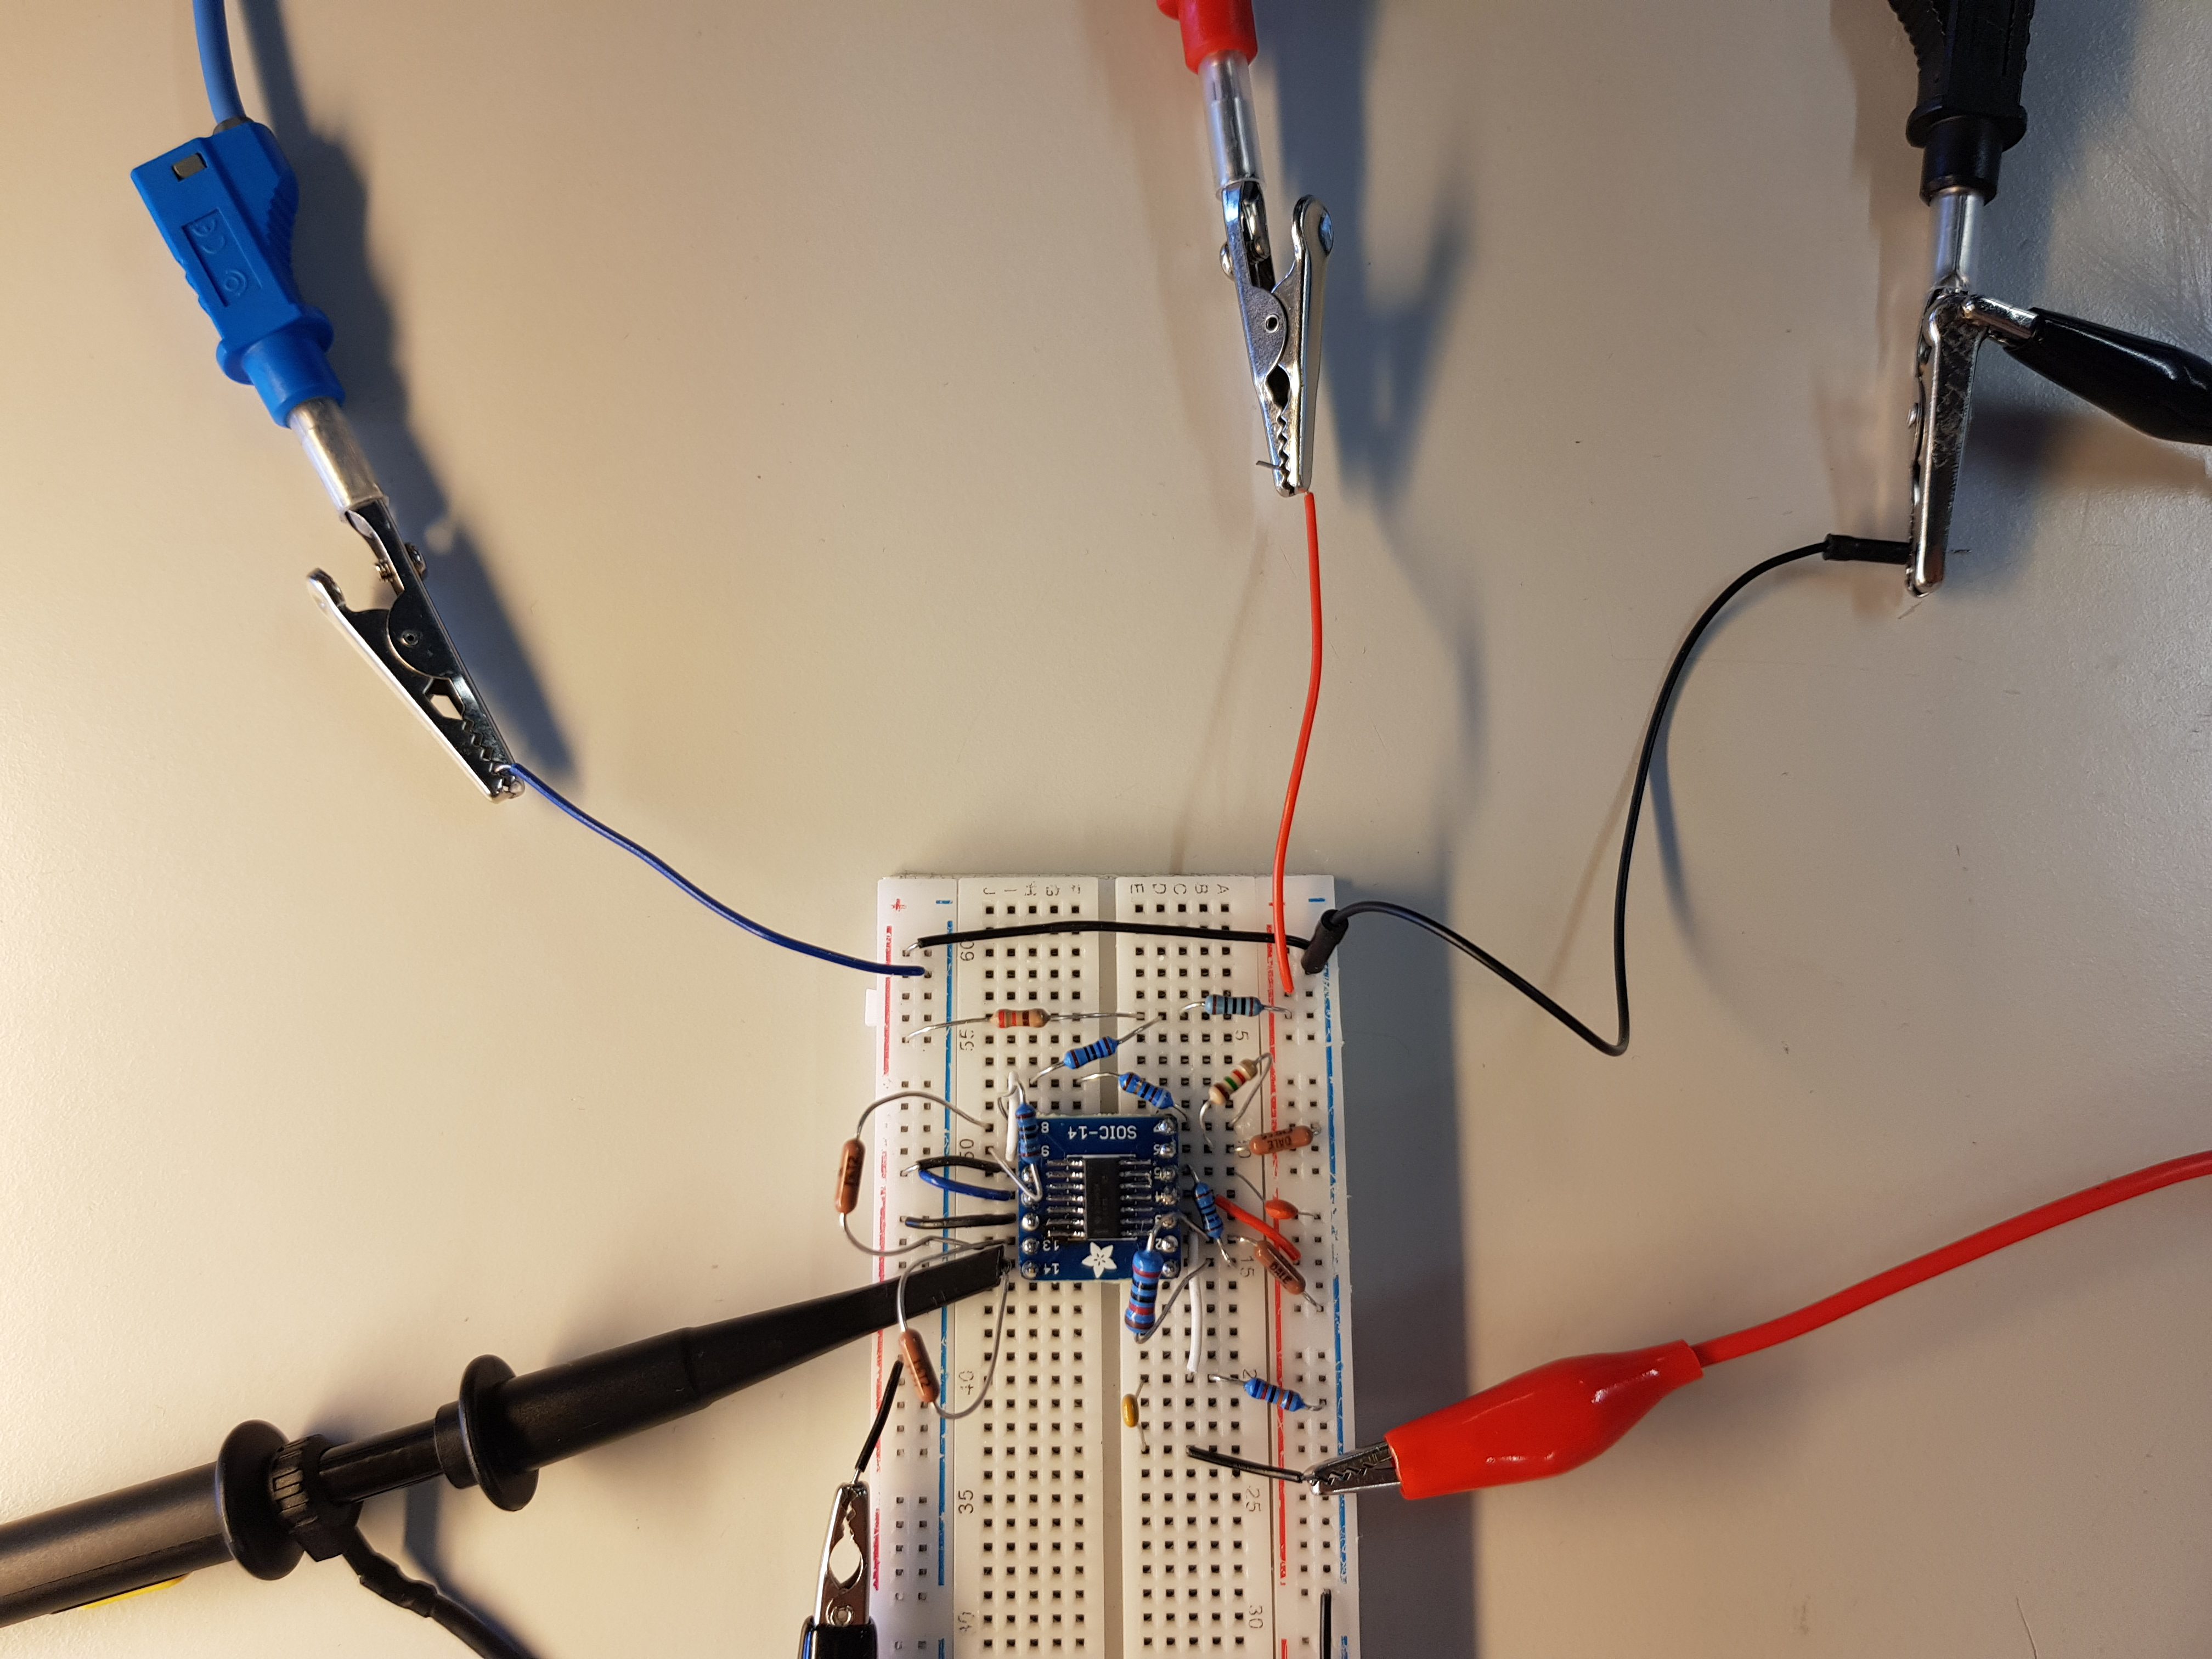
\includegraphics[width=0.7\textwidth]{graphics/TESTINGwSineinp.jpg}
    \caption{Configuration of the noise tests where the circuit is tested, where the probe is connected to the output of the op amps and the input signal is either a sine wave or its connected to ground.}
    \label{fig:SetupFFT}
\end{figure}







The bandwidth of the FFT was set at 100kHz with an input signal being a sine wave with 10$mV_{pp}$ and 20kHz frequency being sent to the input of the op amps.
The results can be seen in \textit{Figure~\ref{fig:Noise20k10mVpp100kband}}, at 20kHz the input signal is apparent with a peak of 3dBm while the noise floor is around -72dBm.
Which yields a SNR, which is the difference between the two amplitudes as 75dB.

\clearpage

\begin{figure}[h]
    \centering
    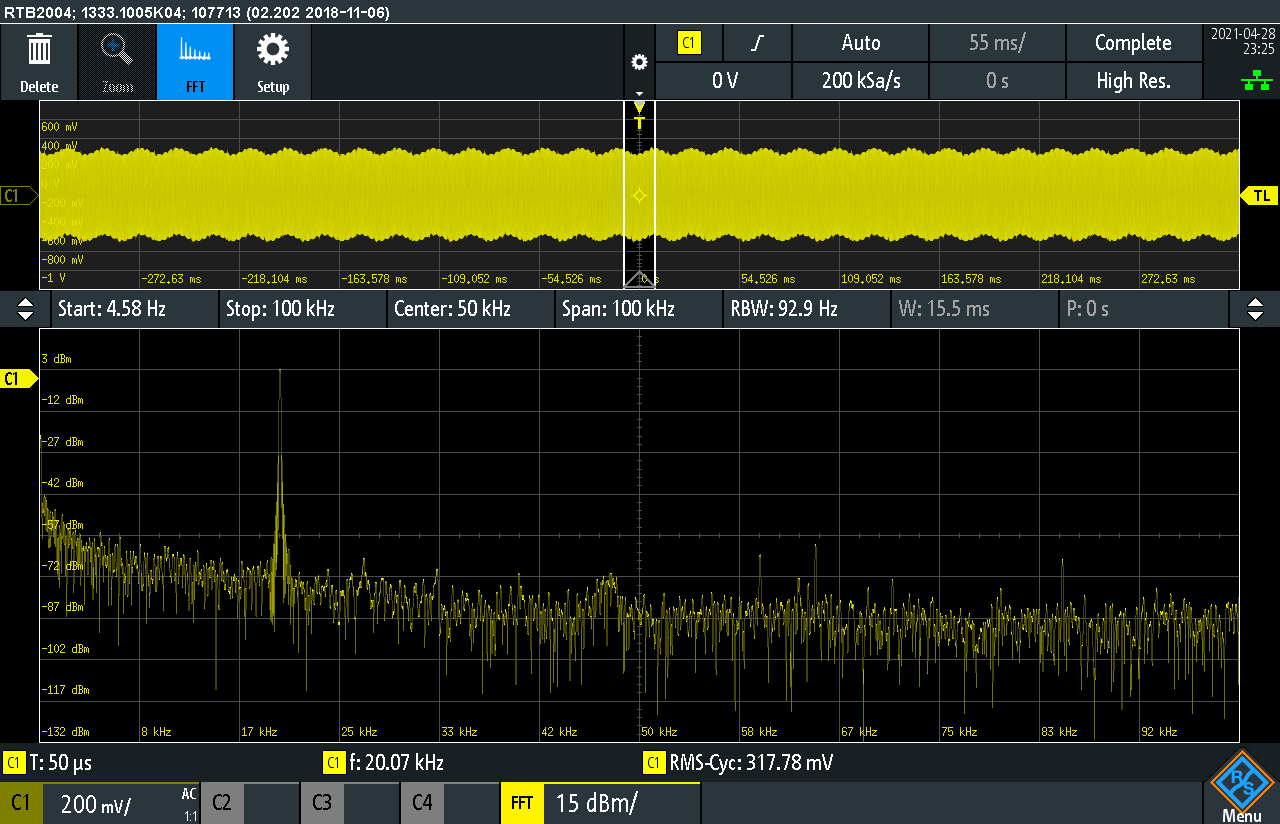
\includegraphics[width=0.7\textwidth]{graphics/Noise20k10mVpp100kband.PNG}
    \caption{FFT on the RTB2004 oscilloscope. An input sine wave signal of 10$mV_{pp}$ and a frequency of 20kHz seen at the top of the figure and the respective FFT below it with a 100kHz bandwidth.}
    \label{fig:Noise20k10mVpp100kband}
\end{figure}



%\begin{figure}[h]
%    \centering
%    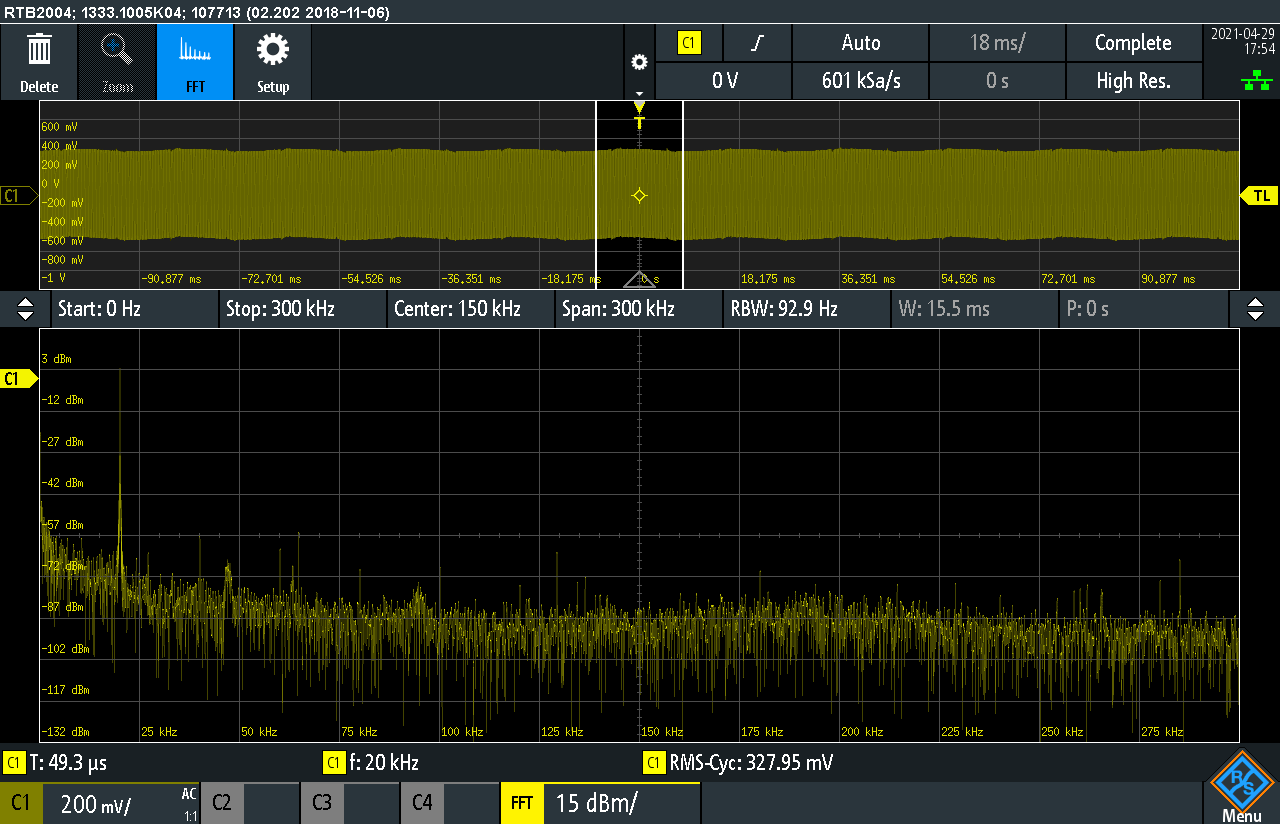
\includegraphics[width=0.7\textwidth]{graphics/Noise20kinp300kBand.PNG}
%    \caption{FFT on the RTB2004 oscilloscope. An input sine wave signal of 10$mV_{pp}$ and a frequency of 20kHz seen at the top of the figure and the respective FFT below it with a 300kHz bandwidth.}
%    \label{fig:Noise20k10mVpp300kband}
%\end{figure}


The same test was performed for just the generator, bypassing the op amp circuit and connecting it directly to the oscilloscope.
The results can be seen in \textit{Figure~\ref{fig:NoiseGenerator20kInp100kBand}}, at 20kHz the input signal is apparent with a peak of -36.8dBm while the noise floor is around -116dBm.
Which yields a SNR of 80dB.

\begin{figure}[h]
    \centering
    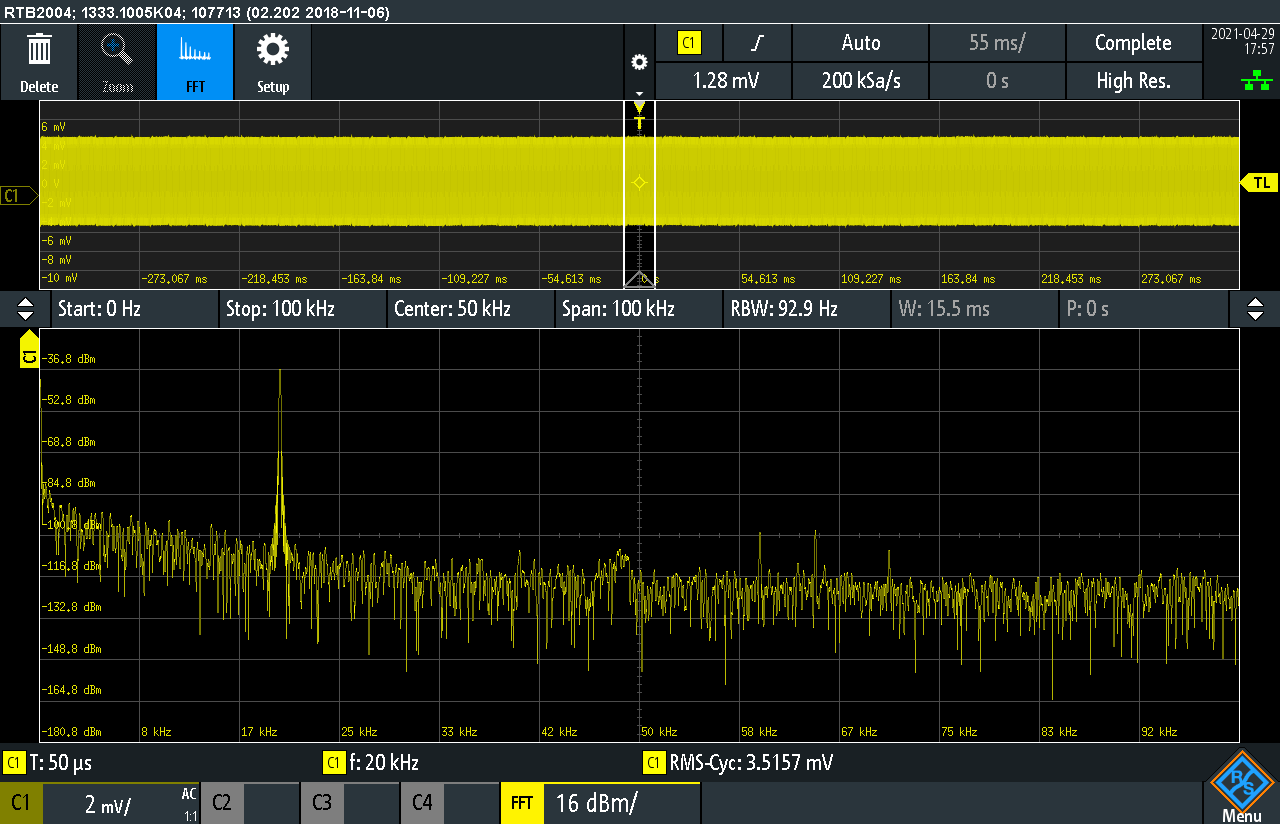
\includegraphics[width=0.7\textwidth]{graphics/NoiseGenerator20kInp100kBand.PNG}
    \caption{FFT on the RTB2004 oscilloscope. 
    An input sine wave signal of 10$mV_{pp}$ and a frequency of 20kHz seen at the top of the figure and the respective FFT below it with a 100kHz bandwidth.}
    \label{fig:NoiseGenerator20kInp100kBand}
\end{figure}

\clearpage

%\begin{figure}[h]
%    \centering
%    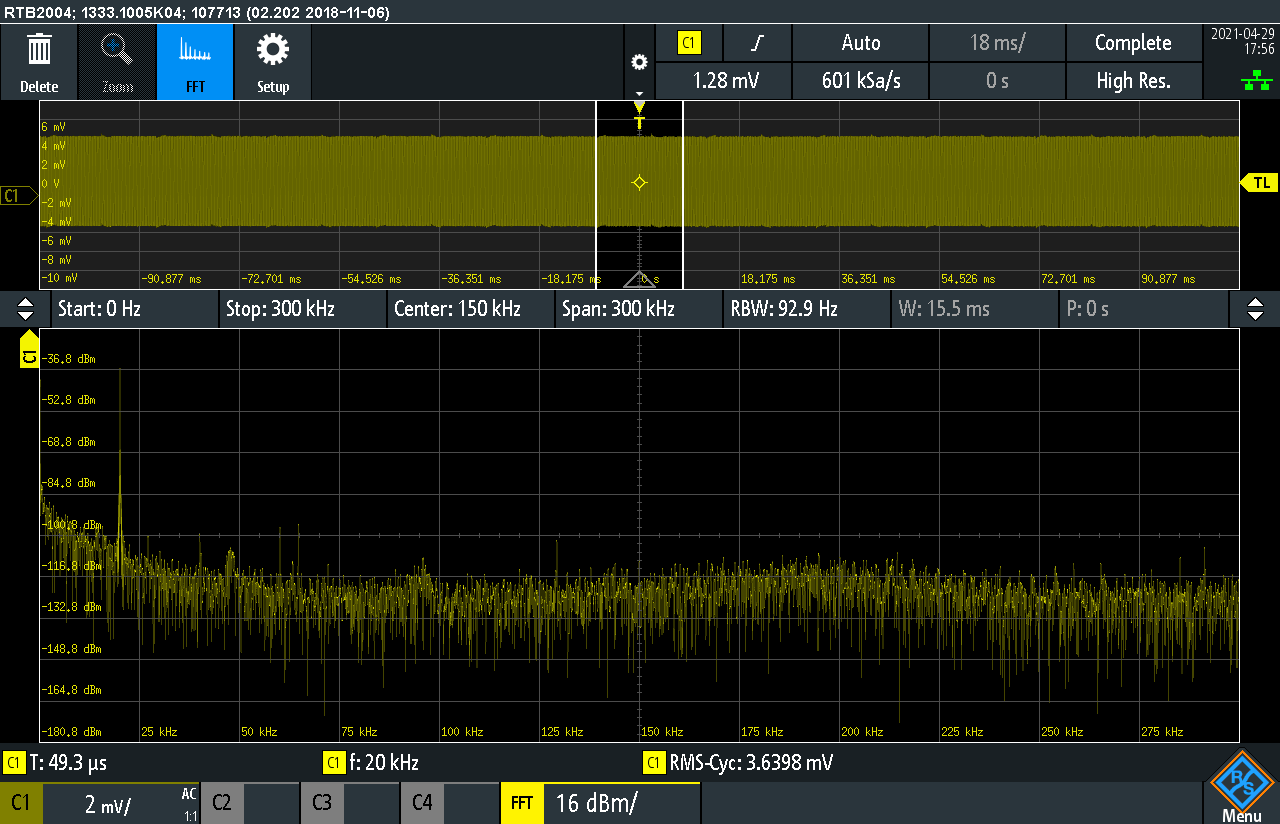
\includegraphics[width=0.7\textwidth]{graphics/NoiseGenerator20kInp300kBand.PNG}
%    \caption{FFT on the RTB2004 oscilloscope. 
%    An input sine wave signal of 10$mV_{pp}$ and a frequency of 20kHz seen at the top of the figure and the respective FFT below it with a 300kHz bandwidth.}
%    \label{fig:NoiseGenerator20kInp300kBand}
%\end{figure}


Now for when the input signal was connected to ground.
The op amps are still getting power from the DC power supply and the probe is connected to the output of the op amps.
The results can be seen in \textit{Figure~\ref{fig:noisefloor100k}}.
This measurement yields a noise floor around of 87.1dBm.


\begin{figure}[h]
    \centering
    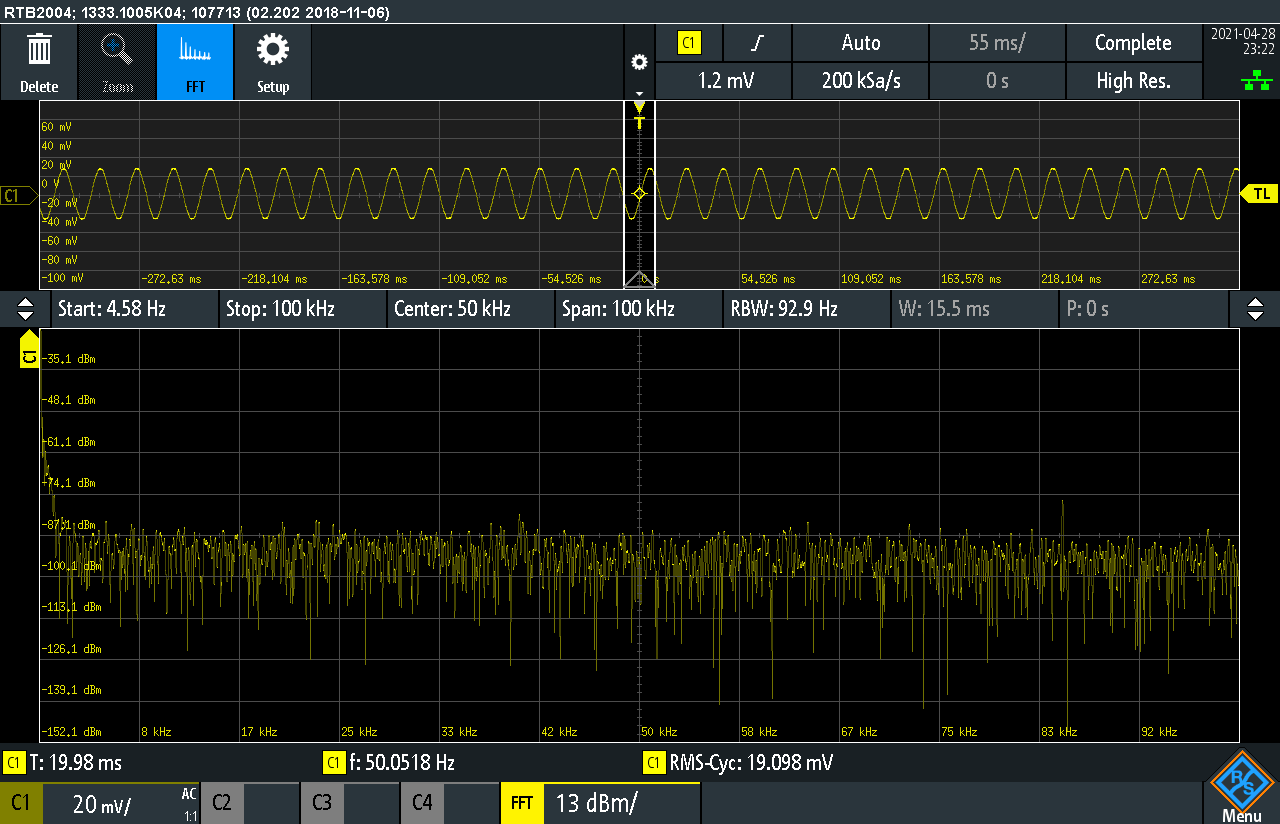
\includegraphics[width=0.7\textwidth]{graphics/NoiseFloor100k.PNG}
    \caption{General noise created by the circuit when op amps are powered and the input is grounded over a frequency band of 100kHz}
    \label{fig:noisefloor100k}
\end{figure}

%Now for when the bandwidth is set to 300kHz.
%Which can be seen in \textit{Figure~\ref{fig:noisefloor100k}}.
%This measurement yields a noise floor of around 86.8dBm.

%\begin{figure}[h]
%    \centering
%    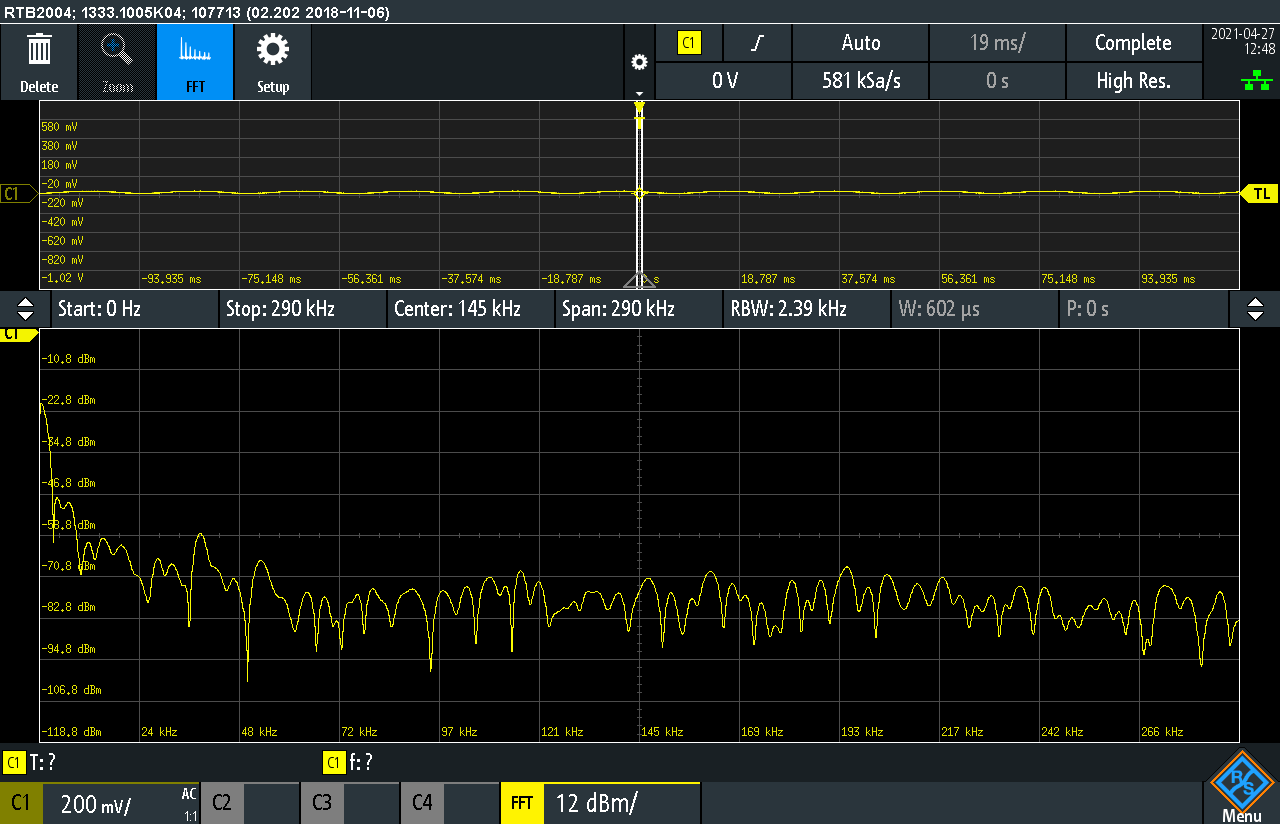
\includegraphics[width=0.7\textwidth]{graphics/NoiseFloor300k.PNG}
%    \caption{General noise created by the circuit when op amps are powered and the input is grounded over a frequency band of 300kHz}
%    \label{fig:noisefloor300k}
%\end{figure}




\clearpage





\subsubsection{Recording signals from a generator}

All tests had the same setup of the device.
The Teensy3.5 was powered via USB, the probe was connected to where input signal was being read and ground was connected to analog reference of the Teensy3.5.
The op amps where powered by the as before by a DC power supply and the input signal was generated by the wave form generator.
The setup of the device with everything connected can be seen in \textit{Figure~\ref{fig:testCircSetup}}.
The Teensy would recorded the record the signal to the SD card, where the values were in hexadecimal.
The output signal of the op amps was then recorded by the RTB2004 oscilloscope.
Ones it had stopped recording the data was transformed from hexadecimal to decimal using the python script seen in \textit{Listing~\ref{src:converHex}} and then plotted using Matlab. script seen in \fxfatal{Bæta Matlab kóða Kanski ekki ???}.


\begin{figure}[h]
    \centering
    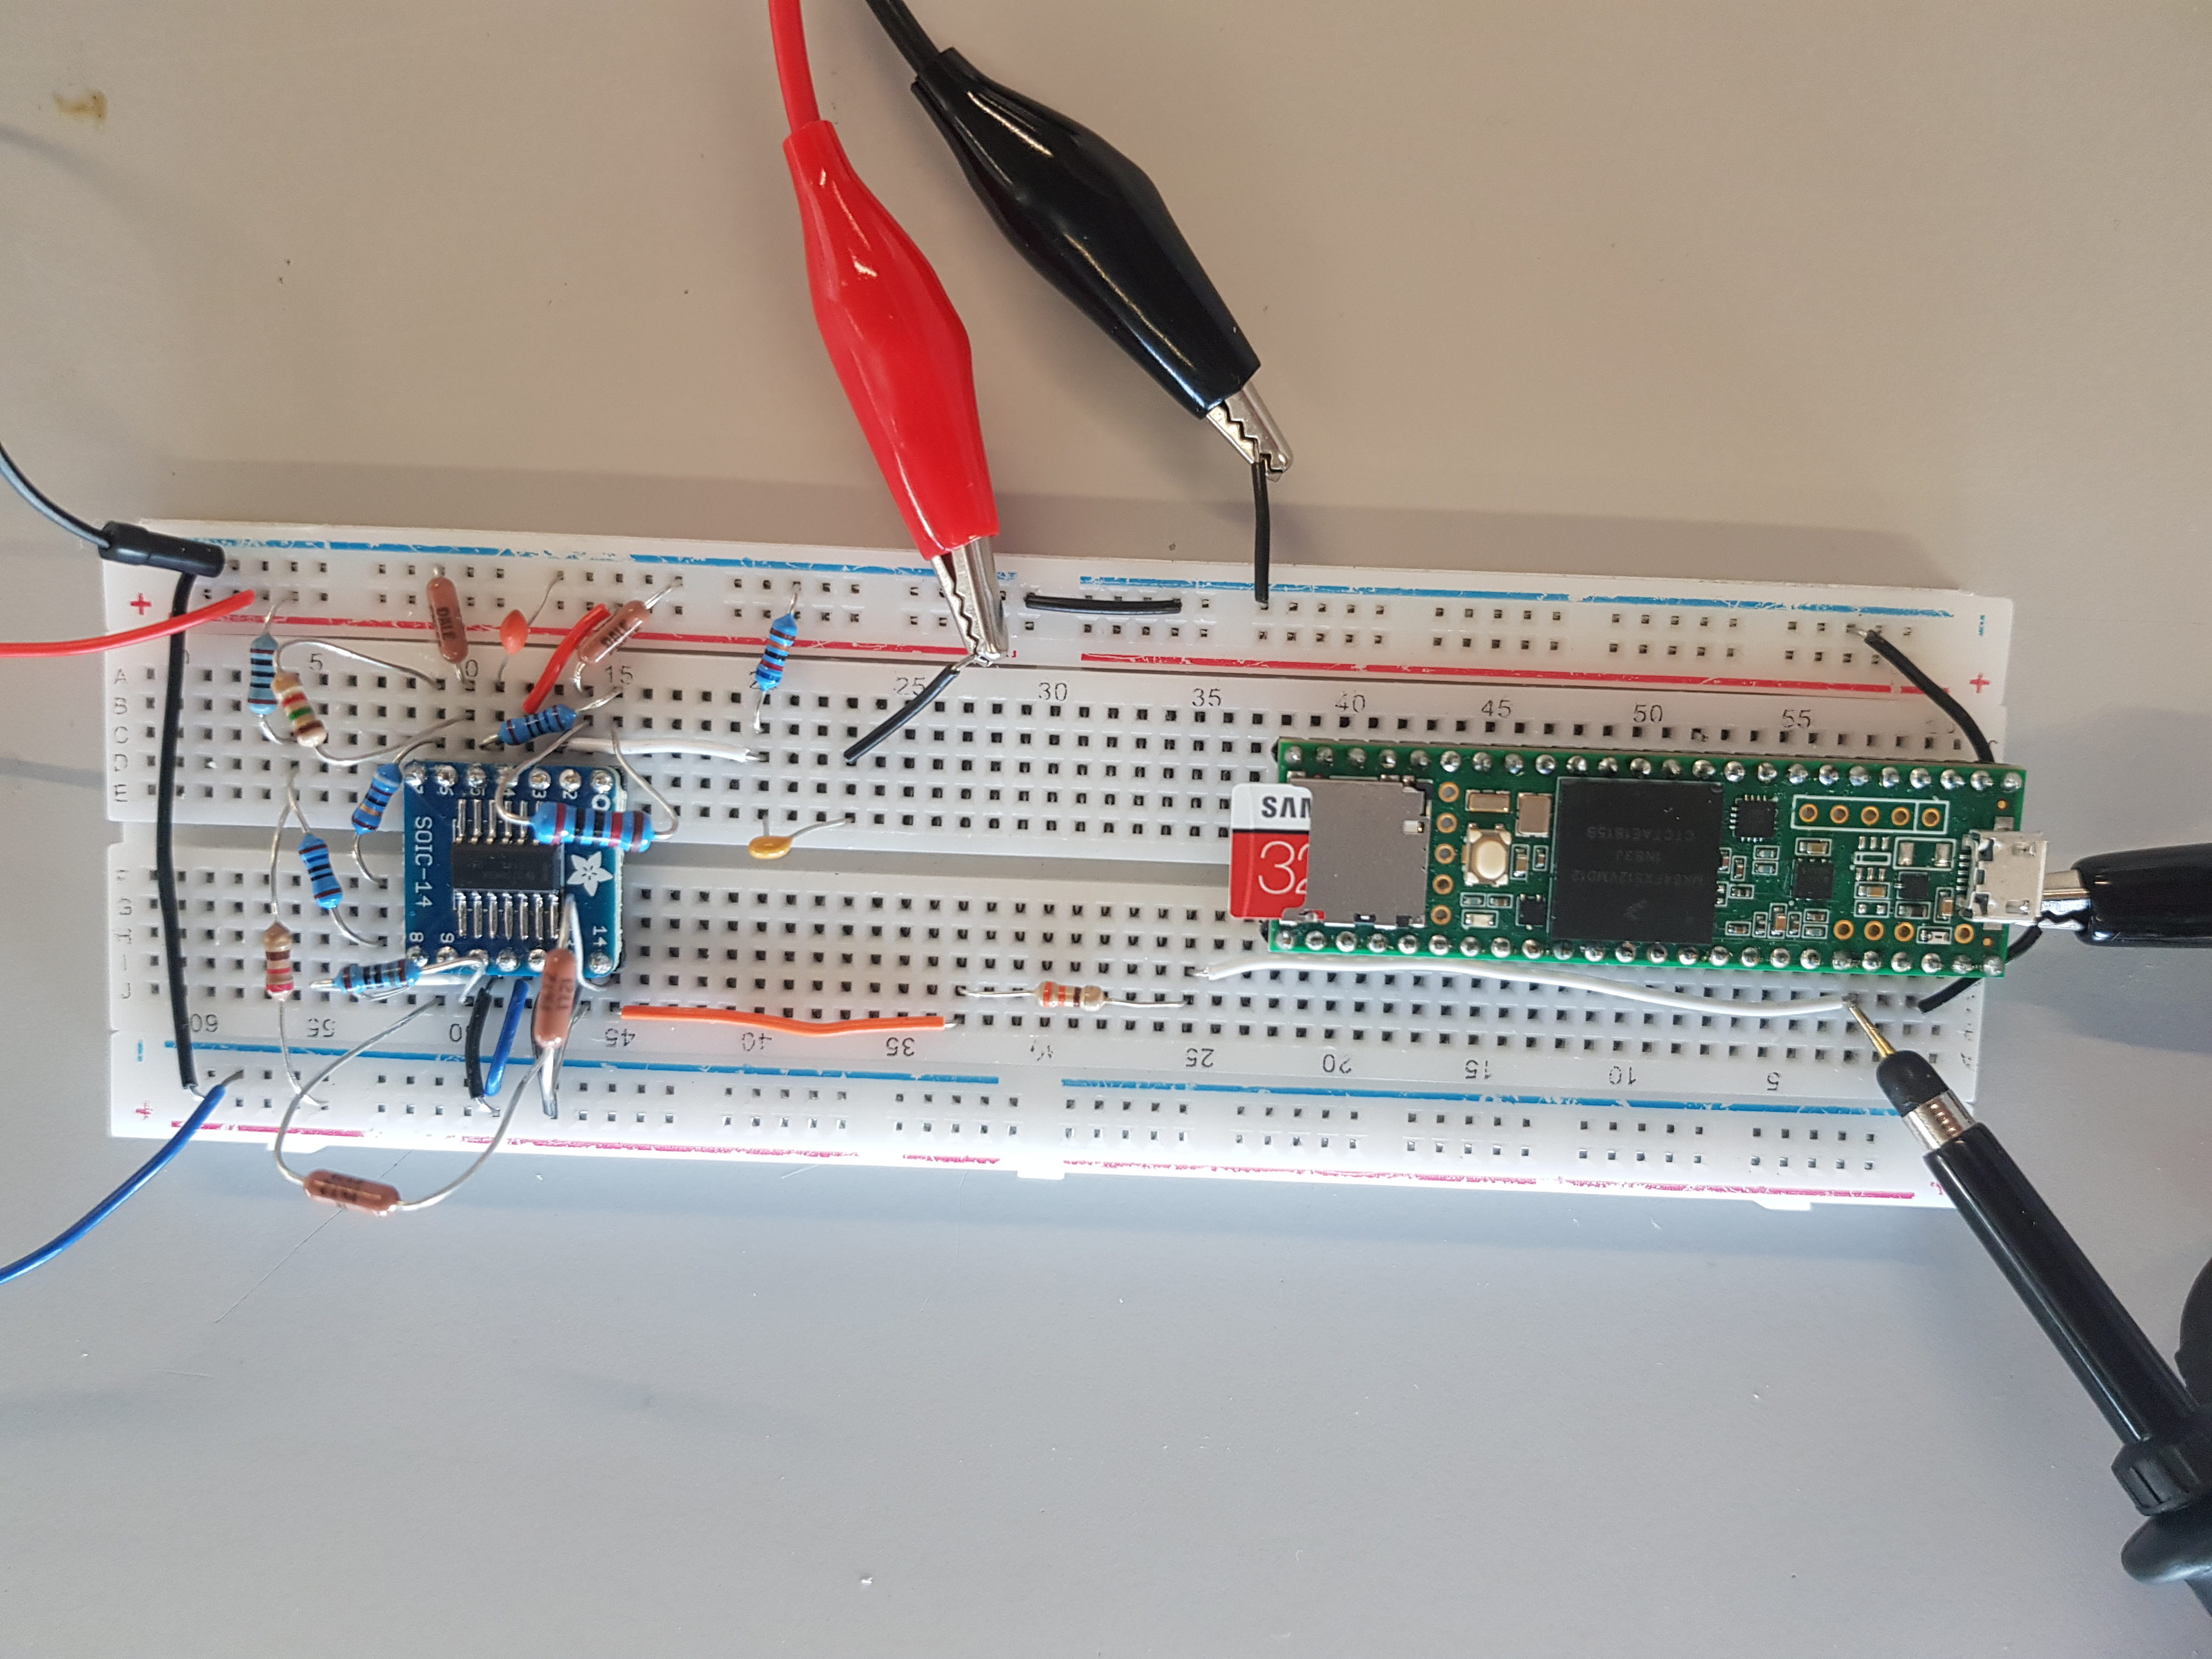
\includegraphics[width=0.7\textwidth]{graphics/TestSetup.jpg}
    \caption{The setup for the circuit for the tests which used the wave form generator as the input signal.}
    \label{fig:testCircSetup}
\end{figure}

In this test it is simulating a 170dB as a source level.
Using the Aquarian H1a as the hydrophone the voltage output would equate to 10mV $V = 10^{170dB-190dB/10} = 10mV$, which was used for all the following tests.
The difference between the three tests was the input signals frequency and the sample frequency of the Teensy.
The first test had the Teensys sample frequency set at 100kHz and a input signal of 10kHz was used.
The data recorded by the Teensy can be seen in \textit{Figure~\ref{fig:Teensy10k100k}}.
While \textit{Figure~\ref{fig:Oscillo10k100k}} shows respective results from the RTB2004 oscilloscope.

\begin{figure}[h]
    \centering
    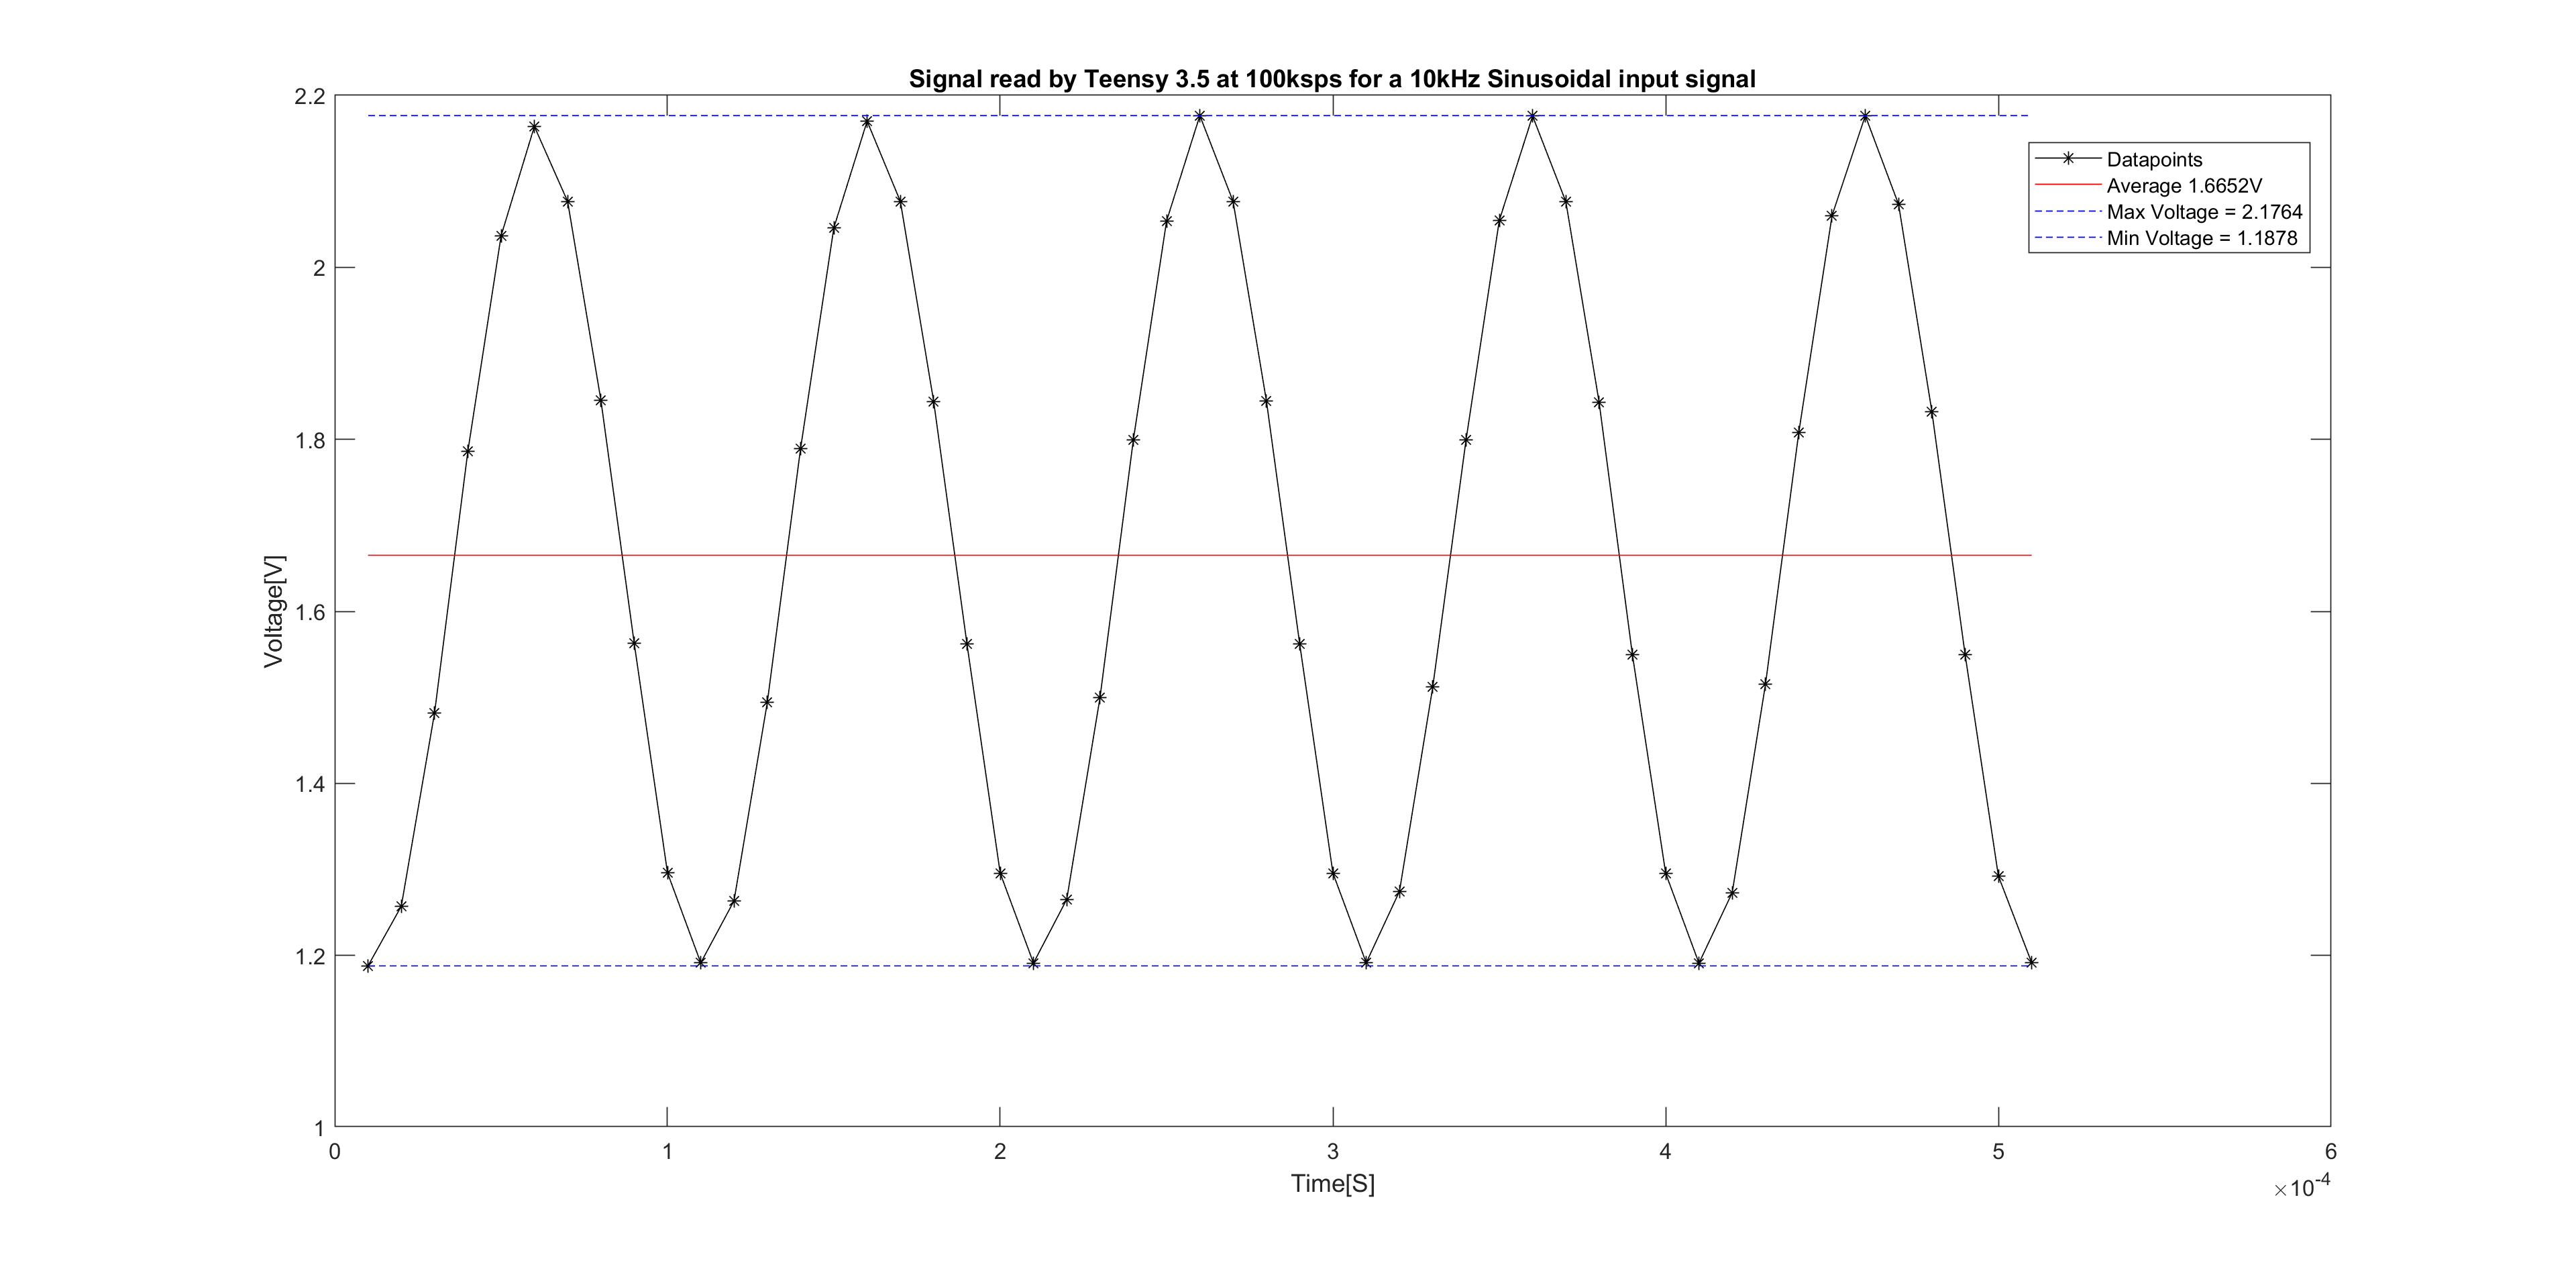
\includegraphics[width=1.0\textwidth]{graphics/10kin_100ksampl.png}
    \caption{Test of the circuit where the input signal was a sinusoidal wave with a frequency of 10kHz and an amplitude of $10mV_{pp}$ and the sample frequency was set as 100kHz}
    \label{fig:Teensy10k100k}
\end{figure}

\begin{figure}[h]
    \centering
    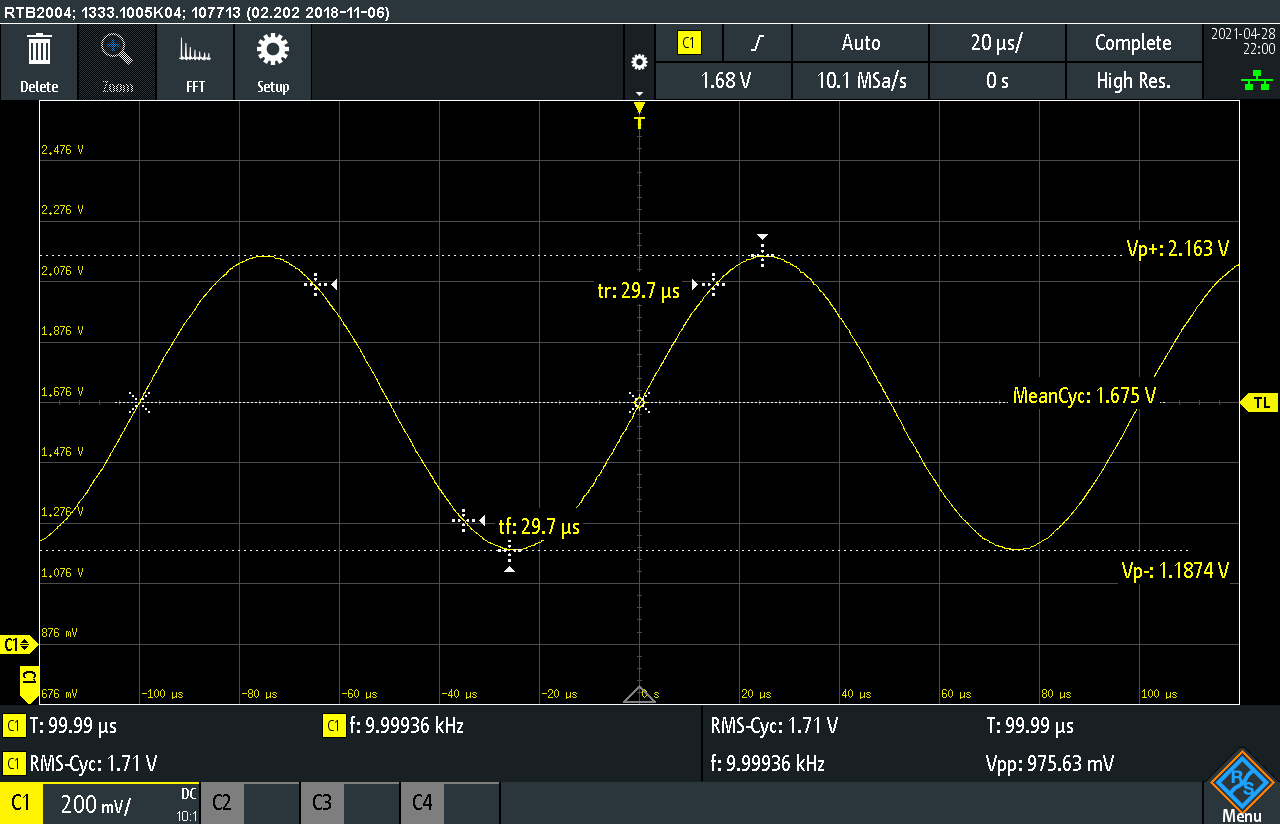
\includegraphics[width=0.7\textwidth]{graphics/10k10mvPP100ksamp.PNG}
    \caption{Shows the results of the oscilloscope scoping, where the probe was connected to the output of the op amp and the input signal was 10kHz.}
    \label{fig:Oscillo10k100k}
\end{figure}

\clearpage



Next the sample frequency was increased to 200kHz and the input signal was 20kHz.
The results of the data recorded by the Teensy can be seen in\textit{Figure~\ref{fig:Teensy20k200k}}.
\textit{Figure~\ref{fig:Oscillo20k200k}} shows respective results from using the oscilloscope for the same input signal as before.

\begin{figure}[h]
    \centering
    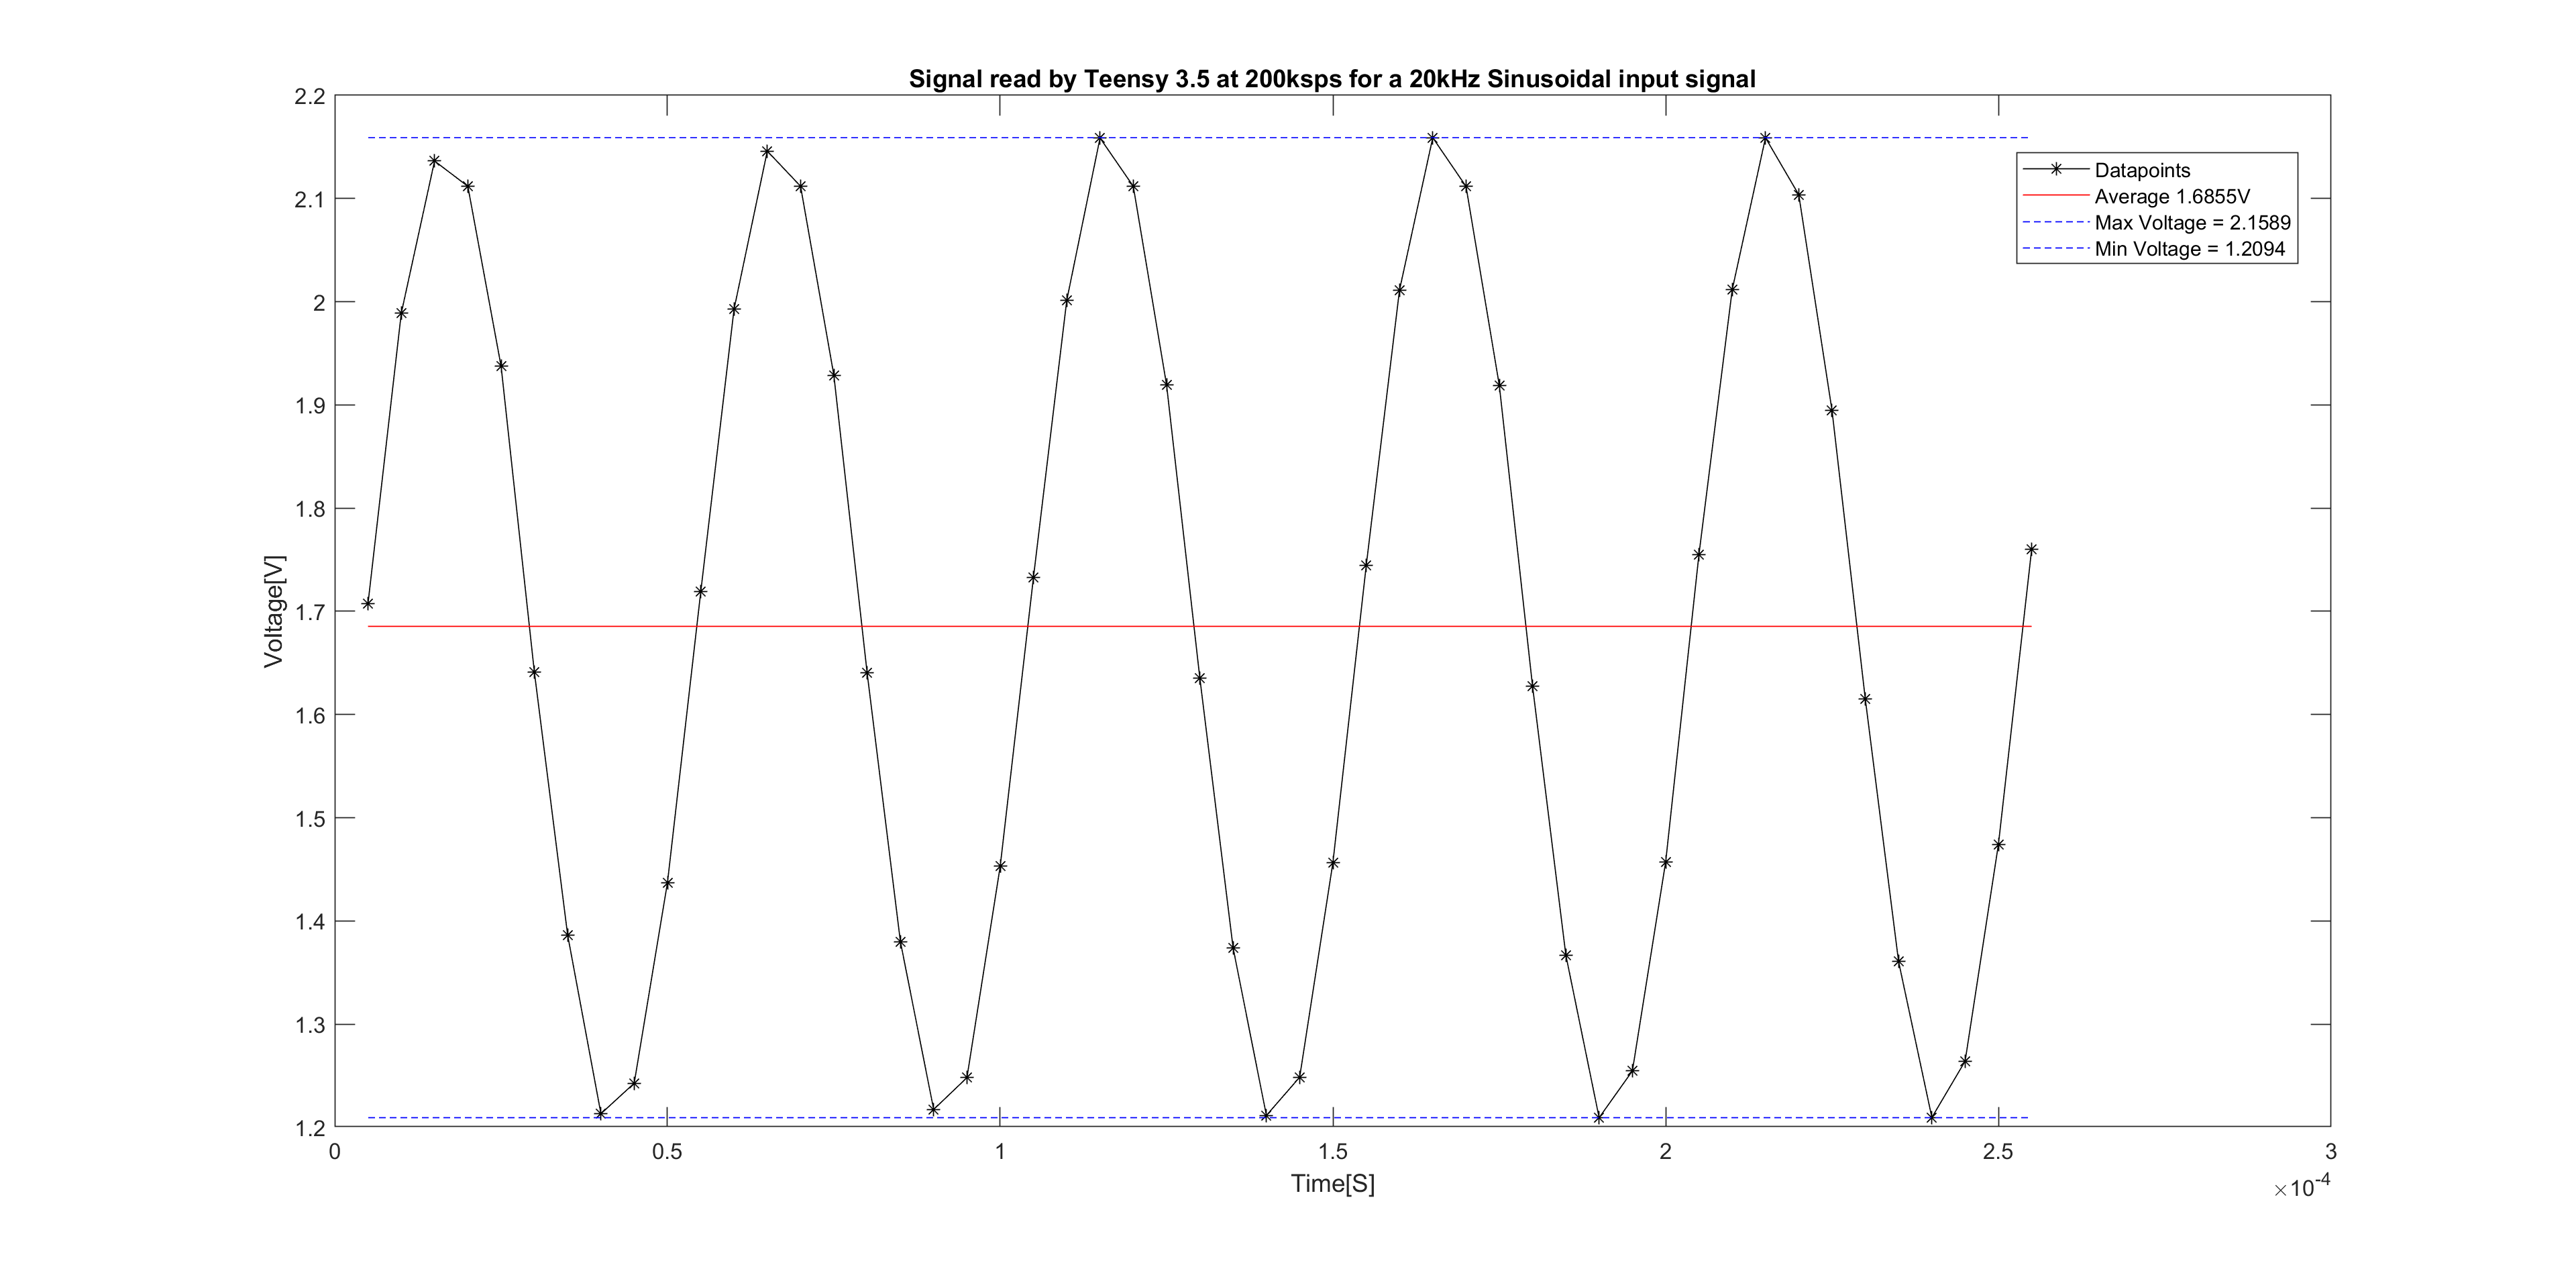
\includegraphics[width=1.0\textwidth]{graphics/20kin_200ksampl.png}
    \caption{Test of the circuit where the input signal was a sinusoidal wave with a frequency of 20kHz and an amplitude of $10mV_{pp}$ and the sample frequency was set as 200kHz}
    \label{fig:Teensy20k200k}
\end{figure}

\begin{figure}[h]
    \centering
    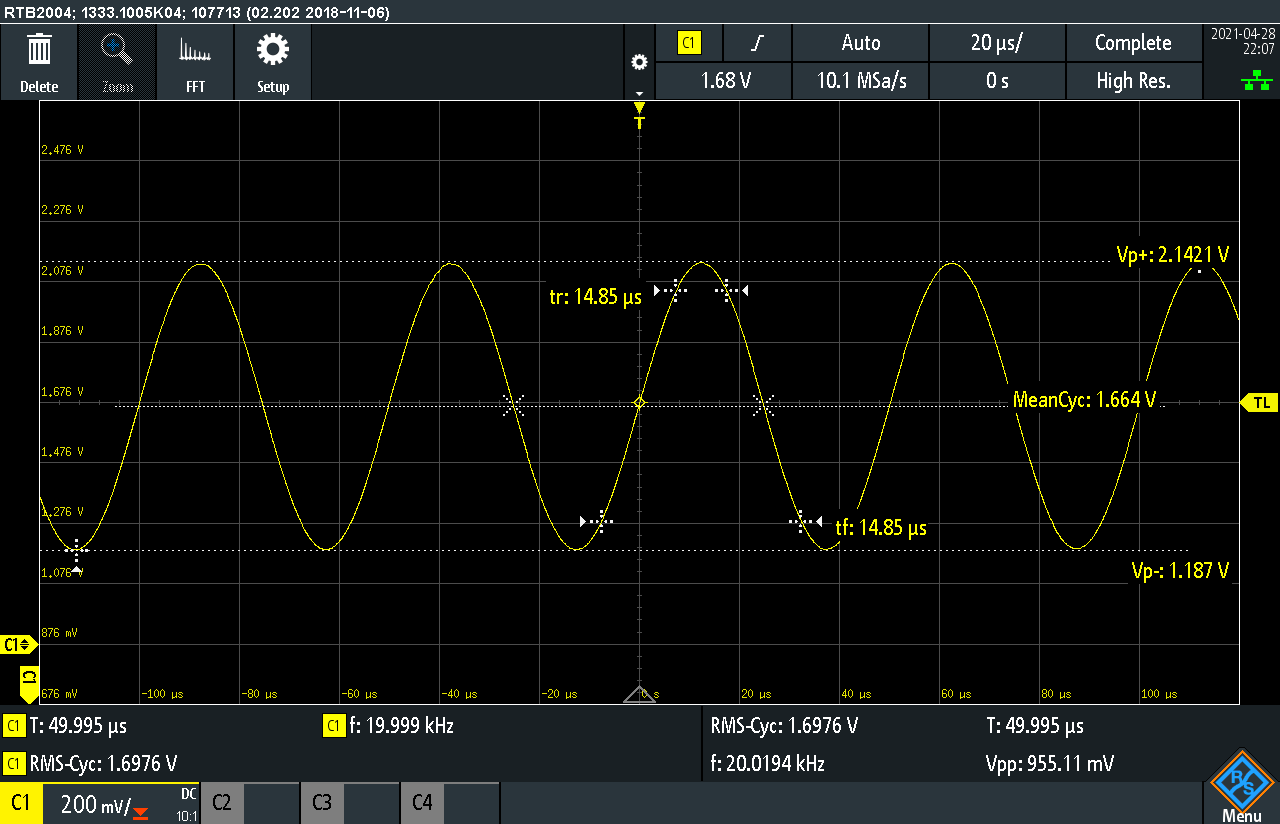
\includegraphics[width=0.7\textwidth]{graphics/20k10mvPP200ksamp.PNG}
    \caption{Shows the results of the oscilloscope scoping, where the probe was connected to the output of the op amp and the input signal was 10kHz}
    \label{fig:Oscillo20k200k}
\end{figure}

\vspace{4cm}



In \textit{Figure~\ref{fig:Teensy30k300k}} the data that the Teensy recorded at 300kHz sample frequency, where the input signal was 30kHz.
\textit{Figure~\ref{fig:Oscillo30k300k}} shows respective results from using the oscilloscope for the same input signal as before.

\begin{figure}[h]
    \centering
    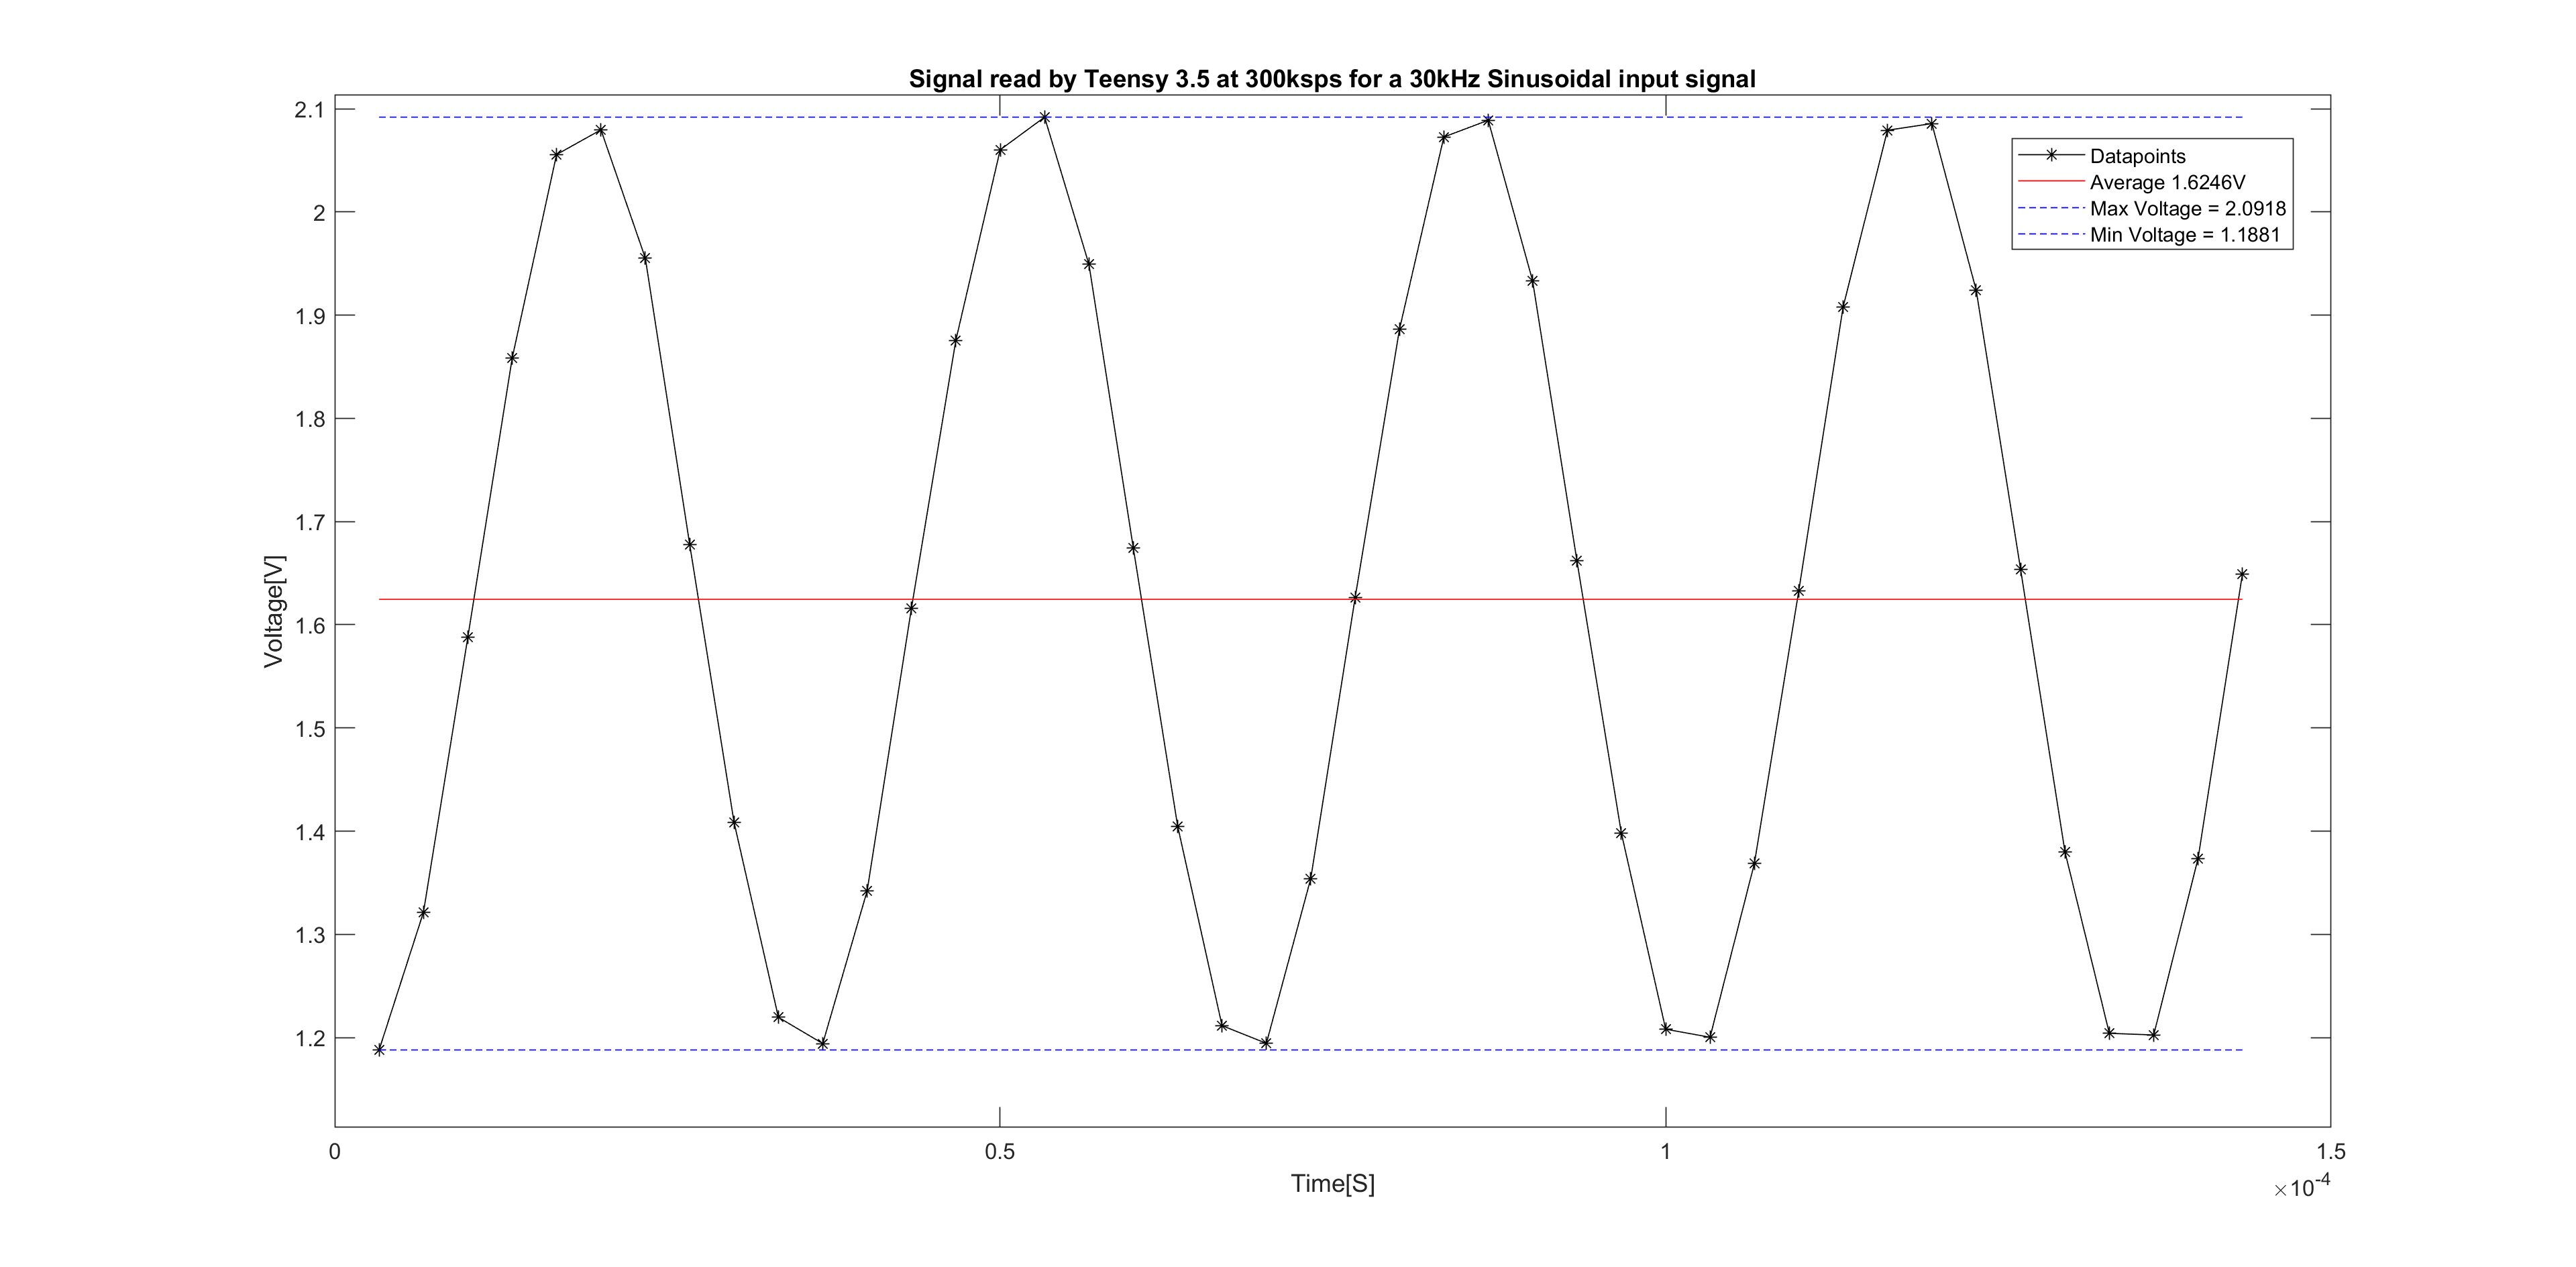
\includegraphics[width=1.0\textwidth]{graphics/30kin_300ksampl.png}
    \caption{Test of the circuit where the input signal was a sinusoidal wave with a frequency of 30kHz and an amplitude of $10mV_{pp}$ and the sample frequency was set as 300kHz}
    \label{fig:Teensy30k300k}
\end{figure}

\begin{figure}[h]
    \centering
    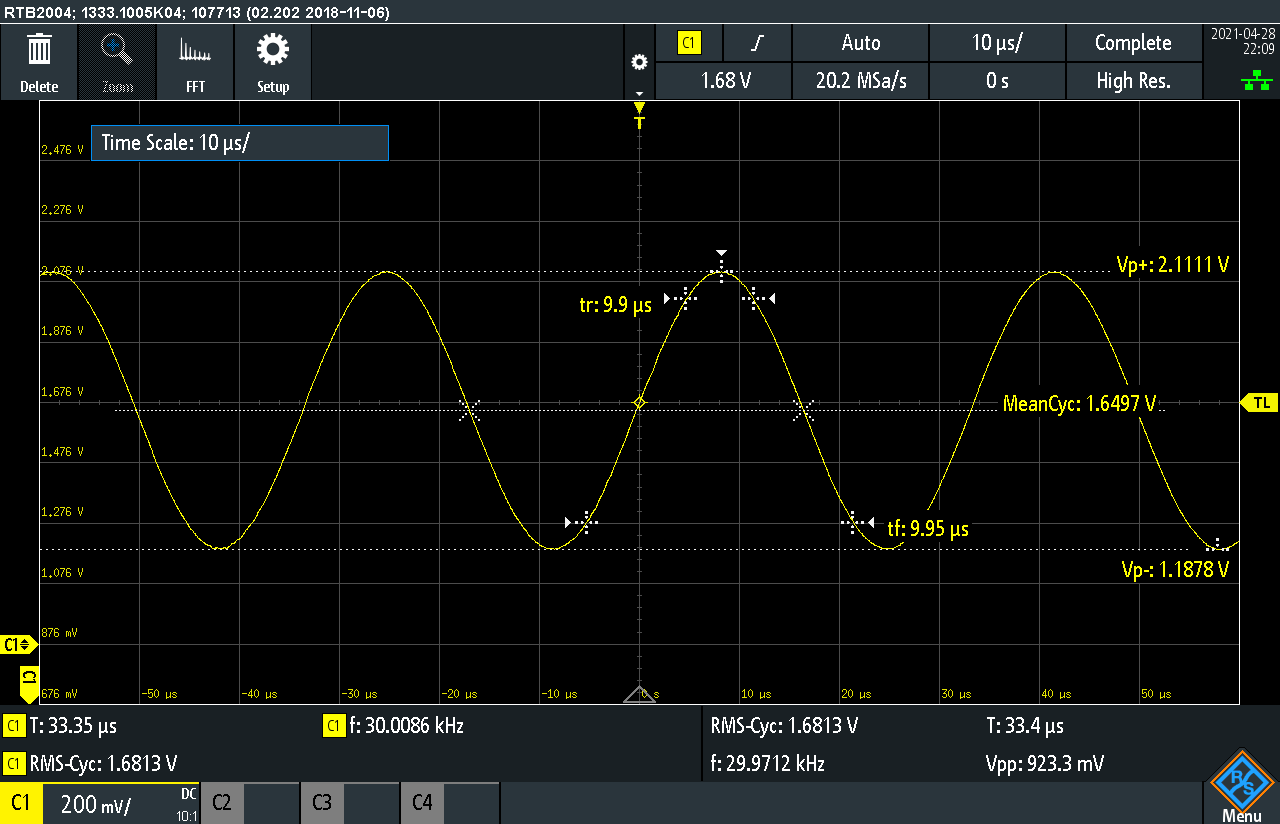
\includegraphics[width=0.7\textwidth]{graphics/30k10mvPP300ksamp.PNG}
    \caption{Shows the results of the oscilloscope scoping, where the probe was connected to the output of the op amp and the input signal was 30kHz}
    \label{fig:Oscillo30k300k}
\end{figure}

\clearpage



Two more tests were performed to better estimate the Teensys accuracy, since at 10mV the signal generator was quite inconsistent and created some variance in its output. \fxfatal{ert með mynd af mælingunni kanski að bæta??}
The test setup can be seen in \textit{Figure~\ref{fig:Last2TestsSetup}}, where the input signal bypasses the op amp circuit and goes straight to the Teensy and Oscilloscope.

\begin{figure}[h]
    \centering
    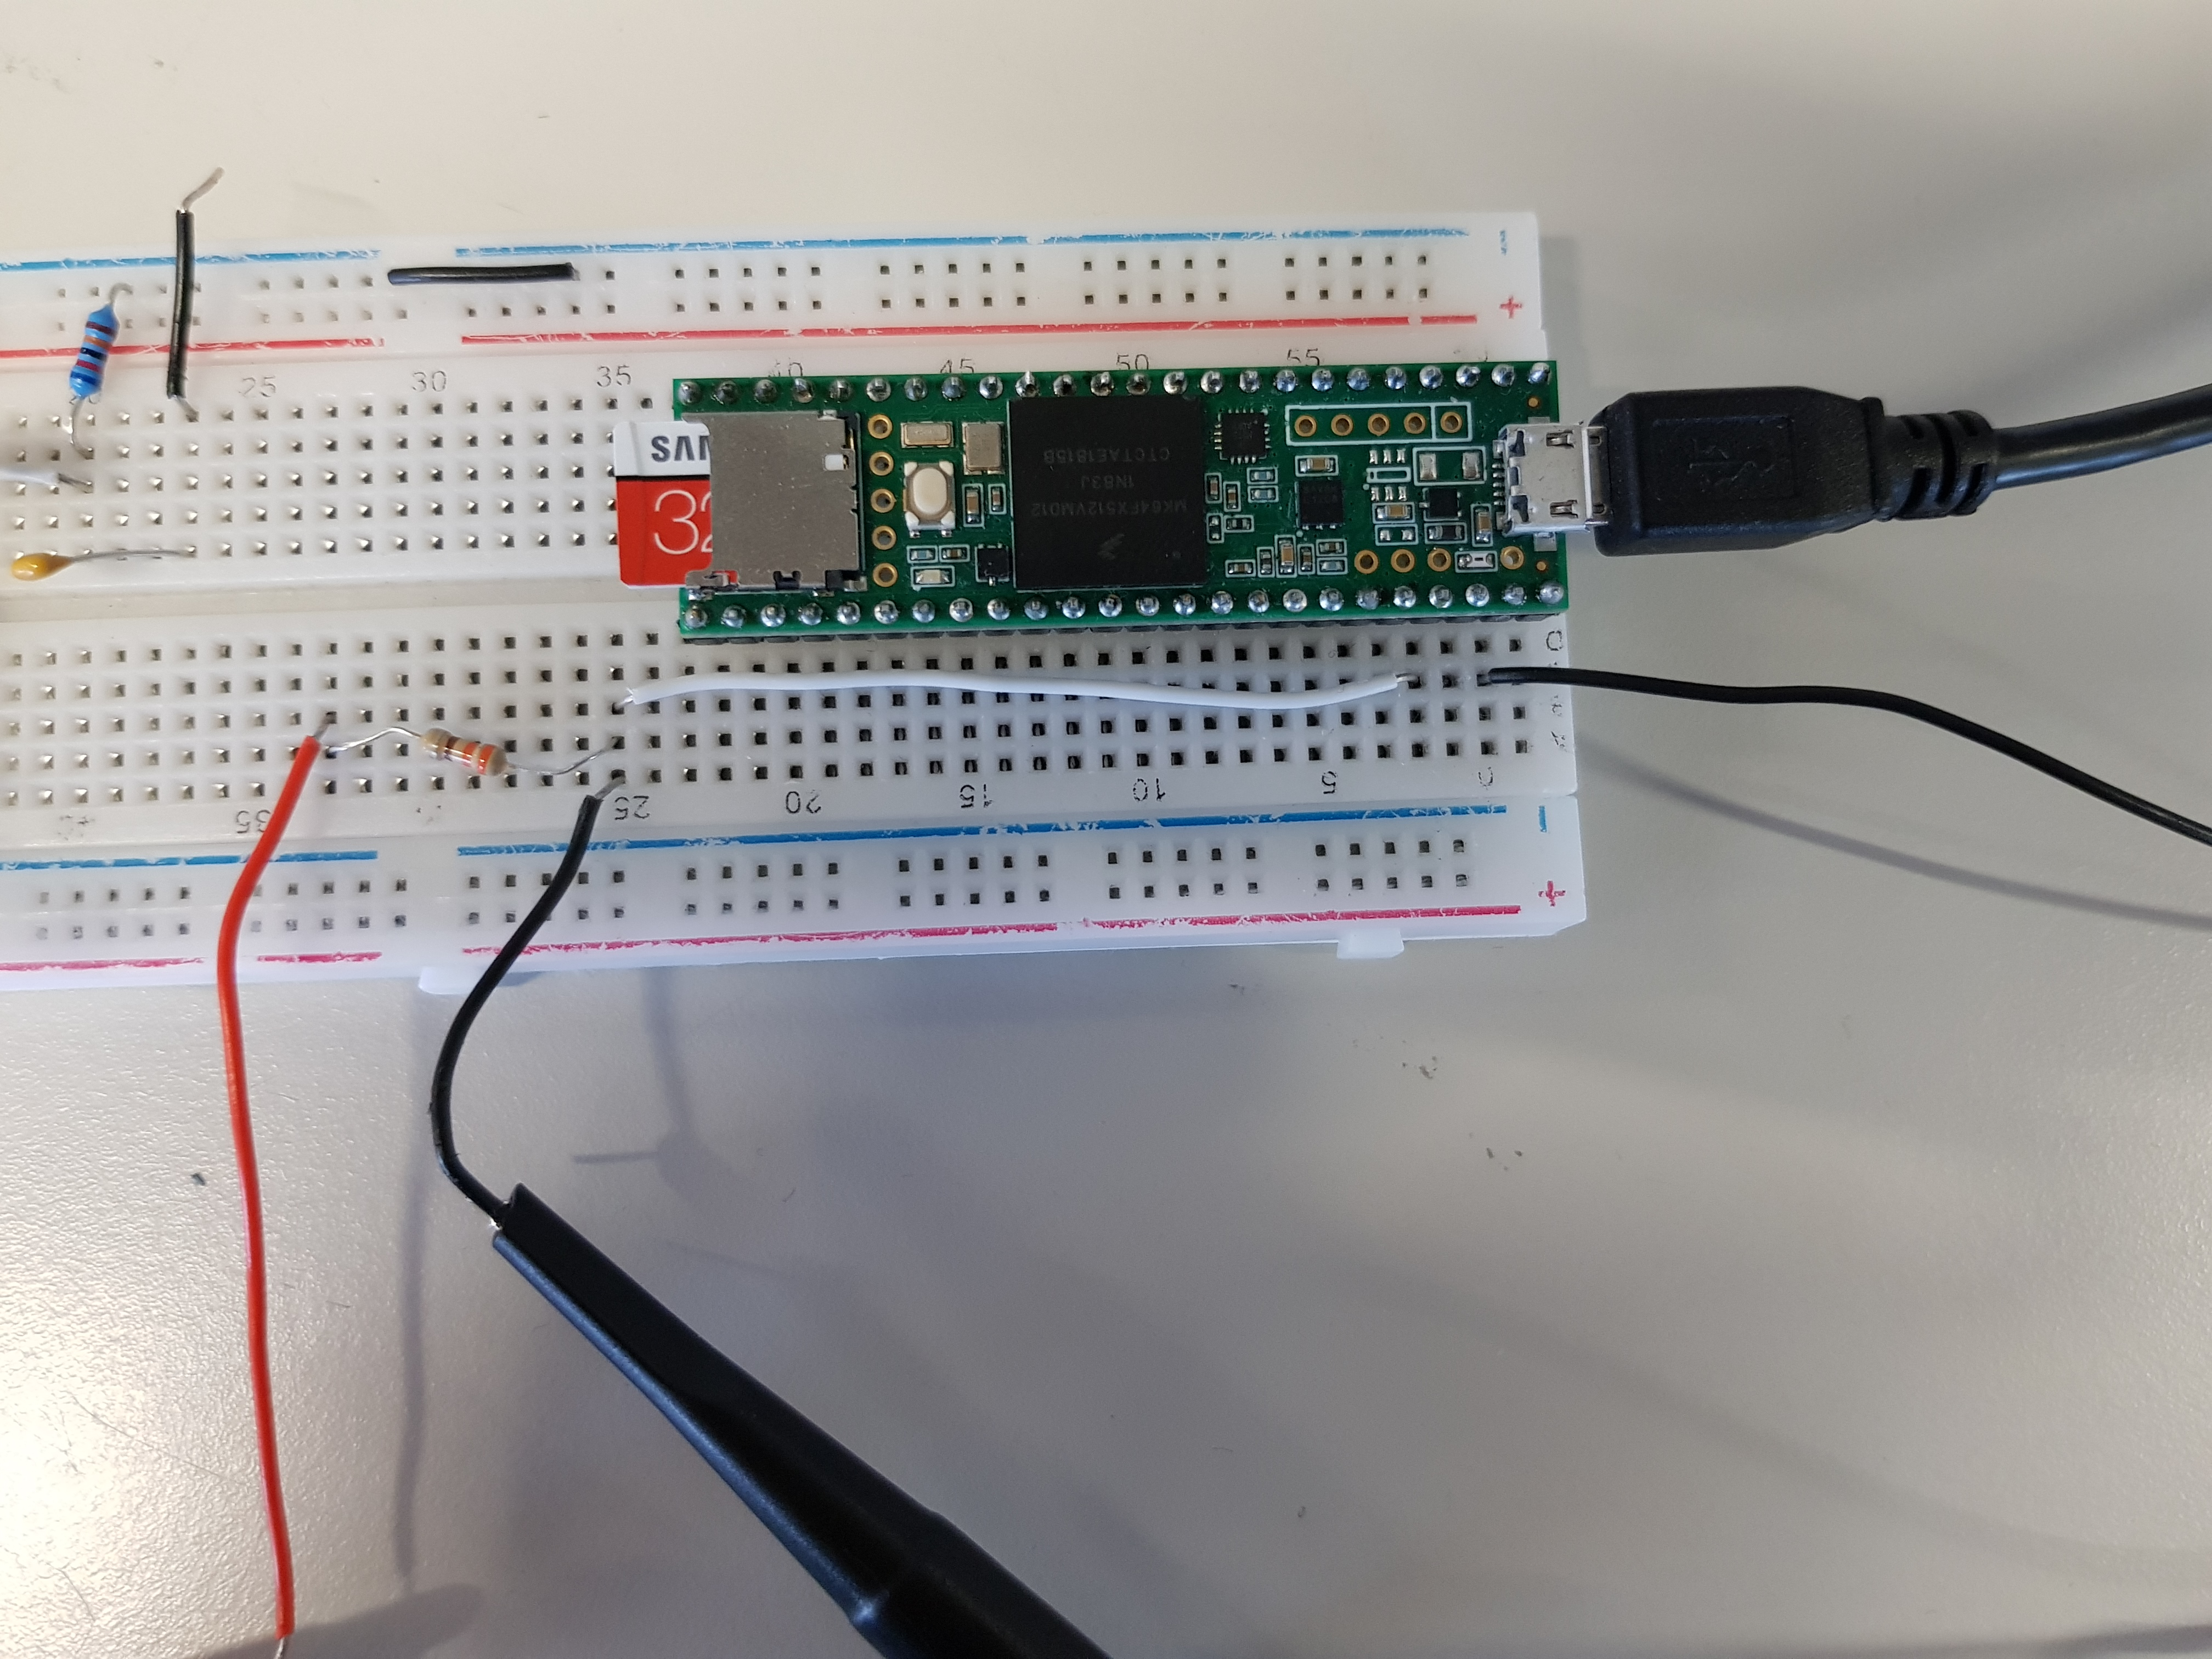
\includegraphics[width=0.7\textwidth]{graphics/Last2Tests.jpg}
    \caption{The input signal connected to the 330$\Omega$ resistor straight to the Teensy.}
    \label{fig:Last2TestsSetup}
\end{figure}


The first signal was a sine wave with 1$V_{pp}$ and VDC offset of 1.65V and 50kHz frequency.
The data plotted from the Teensy can be seen in \textit{Figure~\ref{fig:OscilloCompTeensyAC}}.


\begin{figure}[h]
    \centering
    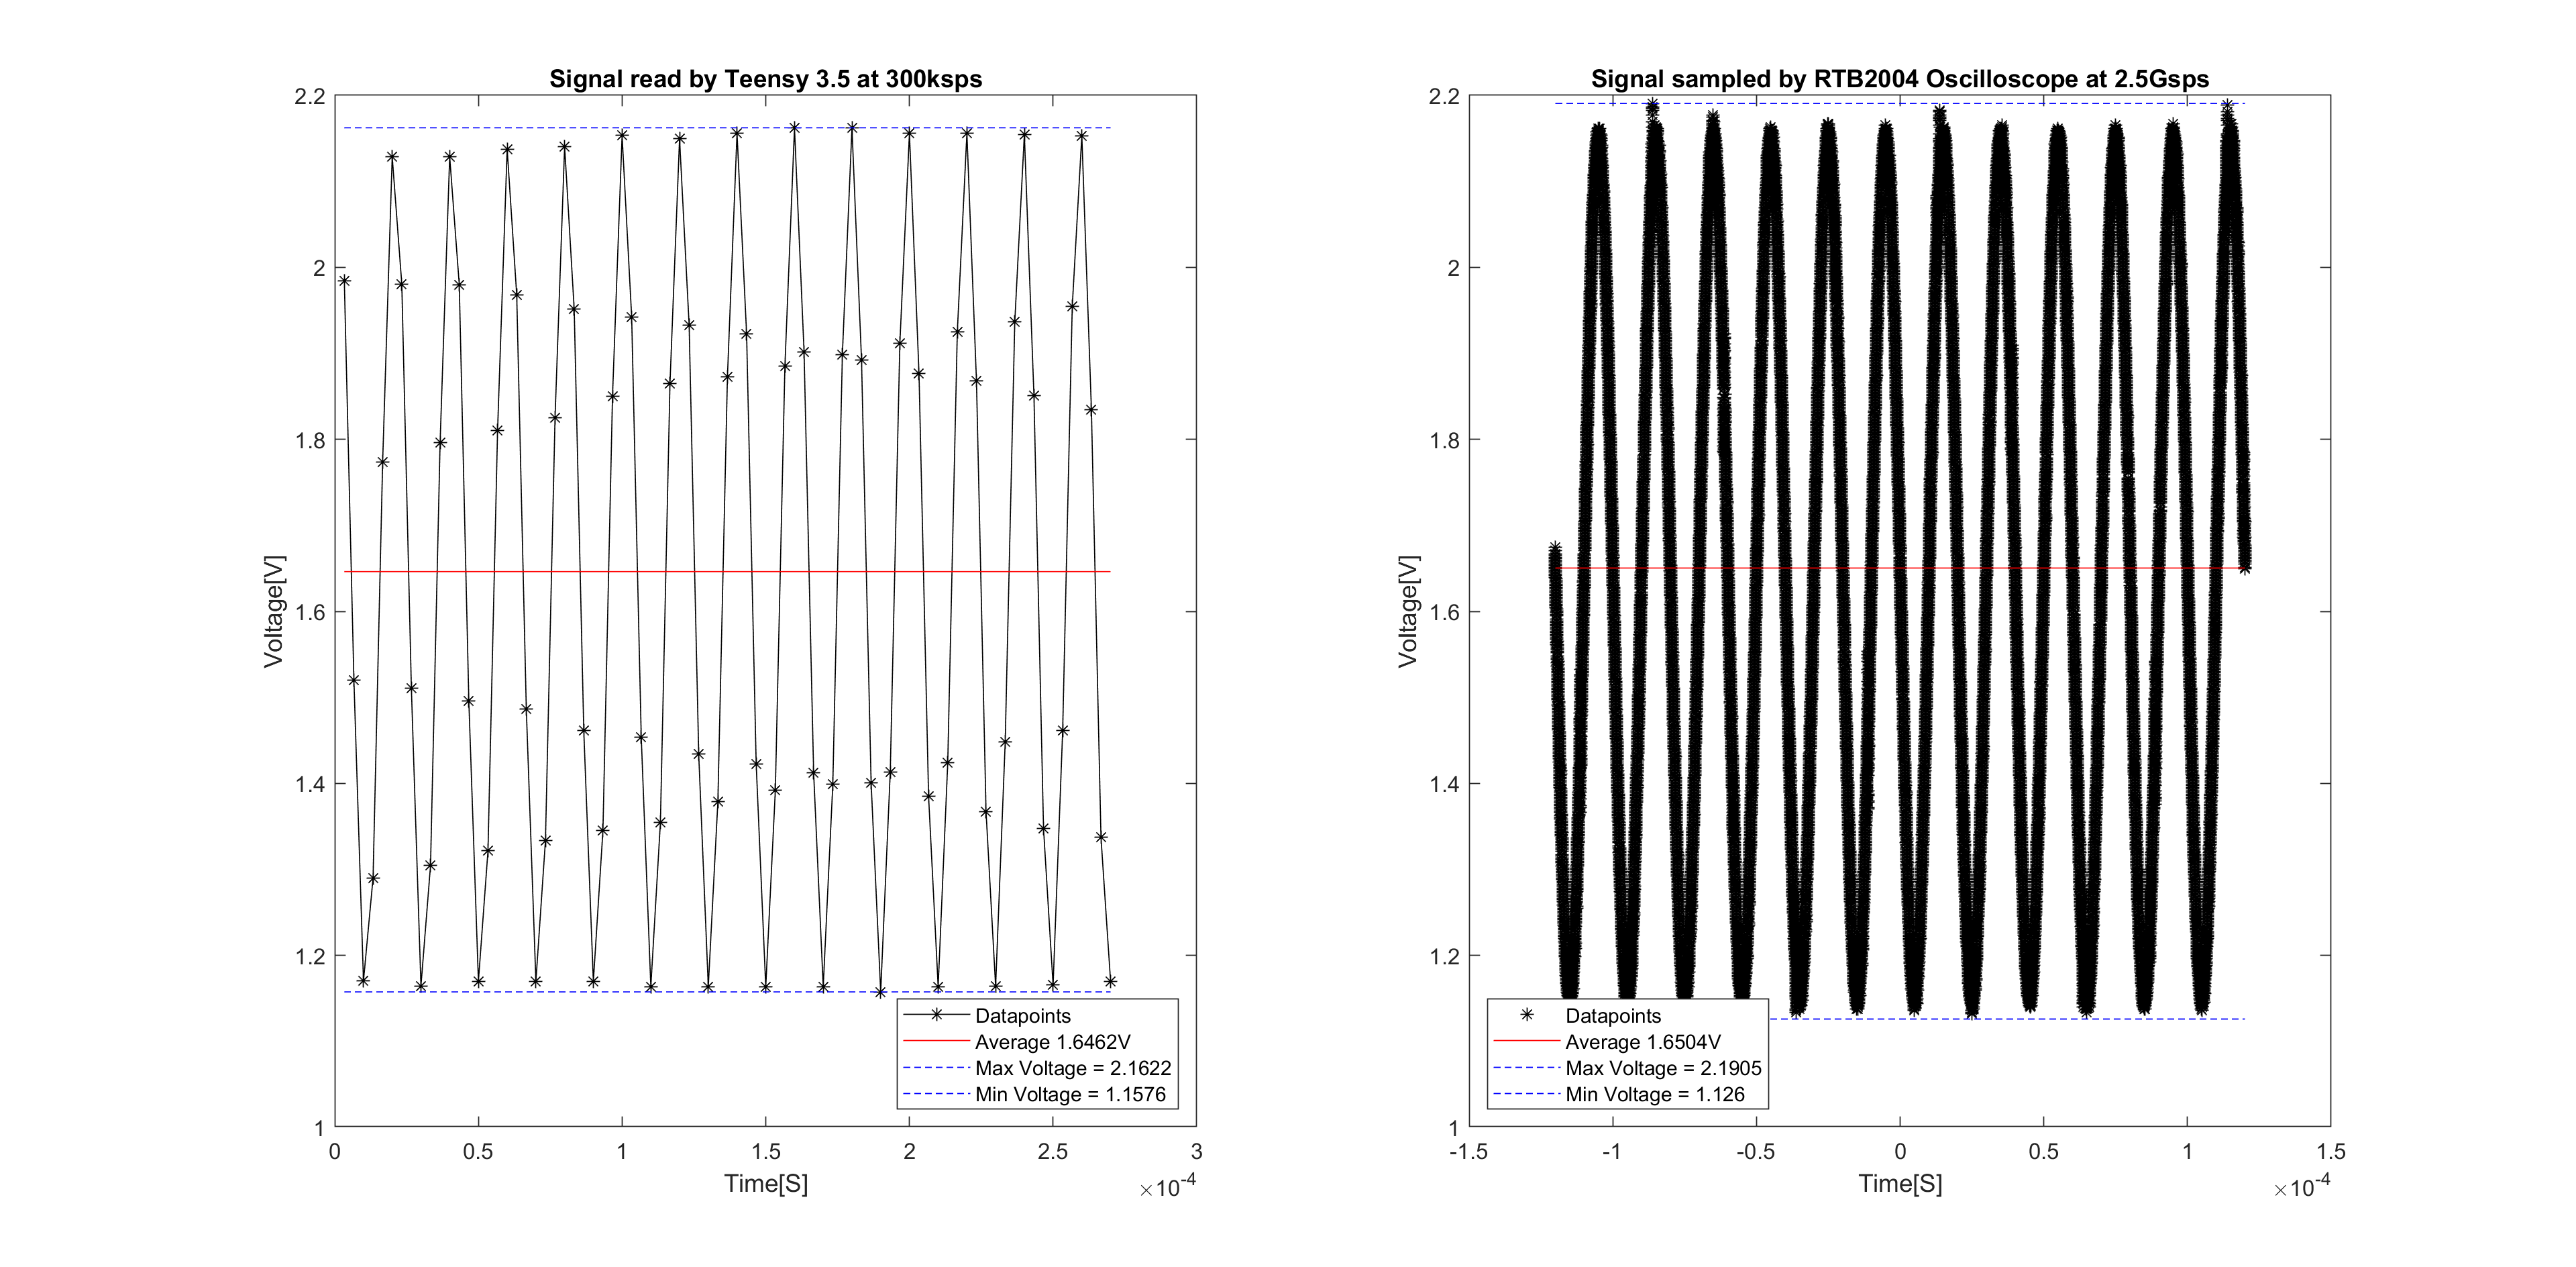
\includegraphics[width=1.0\textwidth]{graphics/OscilloTeensyAC50k1vpp165voffpng.png}
    \caption{With a AC signal of 1$V_{pp}$ and 1.65V DC offset, Teensys readings at 300ksps compared to the RTB2004 oscilloscope at 2.5Gsps}
    \label{fig:OscilloCompTeensyAC}
\end{figure}

The second input signal was DC 1.65V.
The data plotted from the Teensy can be seen in \textit{Figure~\ref{fig:OscilloCompTeensyDC}}.


\begin{figure}[h]
    \centering
    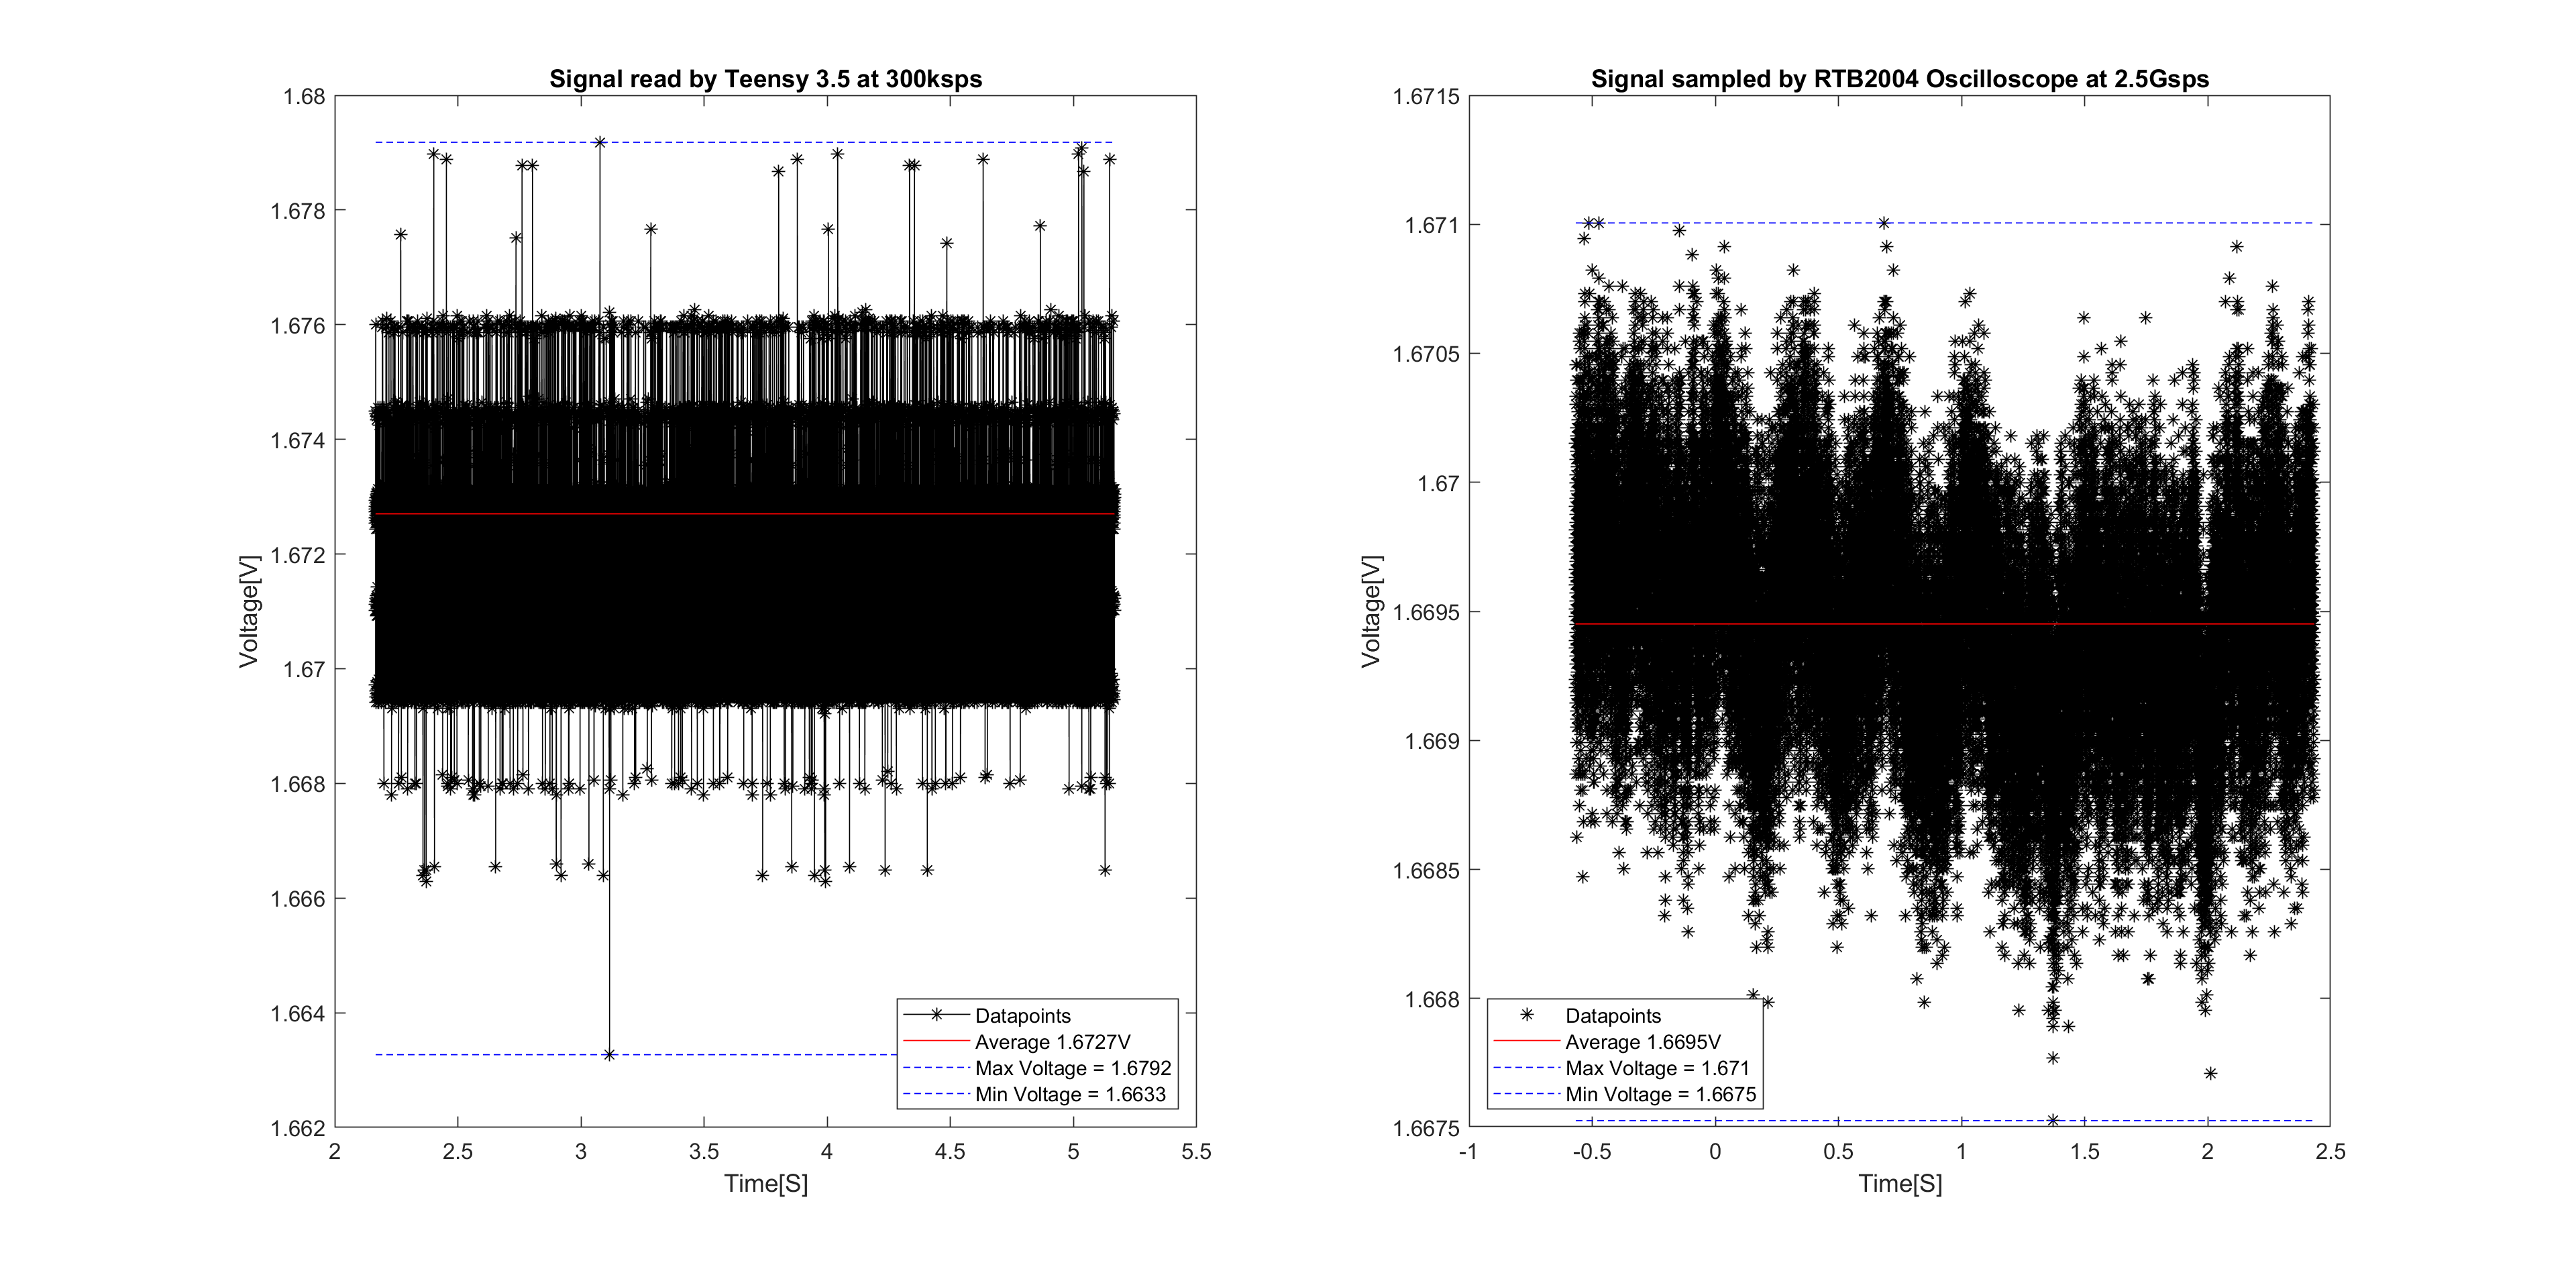
\includegraphics[width=1.0\textwidth]{graphics/OscilloTeensyDC165Read.png}
    \caption{With a DC signal of 1.65V, Teensys readings at 300ksps compared to the RTB2004 oscilloscope at 2.5Gsps}
    \label{fig:OscilloCompTeensyDC}
\end{figure}

%https://www.eevblog.com/forum/beginners/help-with-rapid-adc-data-aquizition/25/
%https://forum.pjrc.com/threads/30171-Reconfigure-ADC-via-a-DMA-transfer-to-allow-multiple-Channel-Acquisition?p=140300#post140300

%TESTa adc_dma_timer í arduino example segja hve hátt þett getur samplað.

%https://github.com/pedvide/ADC/blob/master/AnalogBufferDMA.cpp -> prufa þetta

%%% Local Variables: 
%%% mode: latex
%%% TeX-master: "DEGREE-NAME-YEAR"
%%% End: 
